\documentclass[a4paper, oneside, table]{memoir}

%% Language and font encodings
%% British rather than English fixes date formats
\usepackage[british]{babel}

%%% Margins
\setulmarginsandblock{2cm}{2cm}{*}
\setlrmarginsandblock{3cm}{3cm}{*}
%\setlrmarginsandblock{3cm}{2cm}{*}
\checkandfixthelayout

%% Useful packages
\usepackage{amsmath}
\usepackage{bm}
\usepackage{graphicx}
\usepackage[colorinlistoftodos]{todonotes}
\usepackage[colorlinks=true, allcolors=blue, pdfencoding=auto]{hyperref}
\usepackage{siunitx}
\usepackage{booktabs}
\usepackage[version=4]{mhchem}
\usepackage{listings}
\usepackage{framed}
\usepackage{float}
\usepackage{csquotes}
\usepackage[super]{nth}

% some commands for making tables with alternating colours (replaces tabular environment)
\definecolor{tablegrey}{gray}{0.9}
\let\oldtabular\tabular
\let\endoldtabular\endtabular
\renewenvironment{tabular}{\rowcolors{2}{white}{tablegrey}\oldtabular}{\endoldtabular}
\def\arraystretch{1.2}

%% TIKZ
\usepackage{tikz}
\usetikzlibrary{quotes,angles,decorations.pathmorphing,patterns}
\newcommand{\inputTikZ}[2]{\scalebox{#1}{\input{#2}}}

\usepackage{pgfplots}
\usepgfplotslibrary{dateplot}

%% Bibtex
\usepackage[
backend=bibtex8,
style=phys,
sorting=none,
articletitle=false,
biblabel=brackets,
pageranges=true,
chaptertitle=true
]{biblatex}
\addbibresource{bibliography.bib}
\addbibresource{websites.bib}

\author{Tim Birger Tejsner}
\title{Oxygen Dynamics in the High-Temperature Superconductor LSCO+O}
\date{\today}

%\includeonly{ch/arpes}

\begin{document}

\begin{titlingpage}
    \begin{center}
        \vspace*{1cm}
  
        {\large \textbf{Oxygen Dynamics in the High-Temperature Superconductor LSCO+O}}
  
        \vspace{0.6cm}

        by

        \vspace{0.6cm}
  
        \textbf{Tim Tejsner}

        \vspace{2cm}
  
        \textit{PhD thesis in Physics}
        
        \vfill

        Supervisors: Linda Udby, Andrea Piovano and Martin Boehm
  
        \vspace{1cm}
    
        Niels Bohr Institute\\
        University of Copenhagen\\
        December 2019 
    \end{center}
 \end{titlingpage}

\clearpage

\chapter*{Abstract}

\clearpage

\tableofcontents

\clearpage

% \listoffigures
% \listoftables
\listoftodos

\chapter{Introduction}

In this thesis, we explore certain aspects of the so-called high-temperature superconductors. While these materials were discovered fairly recently (1986), they have a rich history with hundreds of thousands of citations and, to this day, a lively debate surrounding the microscopic nature of this mysterious macroscopic quantum state. The purpose of this chapter is to briefly state the `the story so far' in broad strokes, and then dive deeper into state-of-the-art research relevant for the work performed in this thesis.

\section{Superconductivity}
Superconductivity is a state of matter where a material is able to conduct electricity with \emph{zero} resistance below a certain critical temperature $T_\text{c}$. Since we, fortunately, live in a world where the `spherical cow in a vacuum' model does not apply, it is remarkable to find \emph{real} materials where electrons can propagate without friction. In fact, experiments have shown, that under the right conditions it is possible to keep a persistent superconducting current running for 100000 years \cite{File1963}!

Superconductivity was first discovered in 1911 by Kamerlingh Onnes, essentially as a consequence of being able to liquefy helium in 1908 and reach temperatures close to absolute zero (see \cite{VanDelft2010} and references therein for a breakdown of the experiments). His low-temperature measurement of lead revealed a sudden drop in resistivity at \SI{4.2}{\kelvin}, as seen in the historic plot on figure \ref{fig:onnes}

\begin{figure}
    \centering
    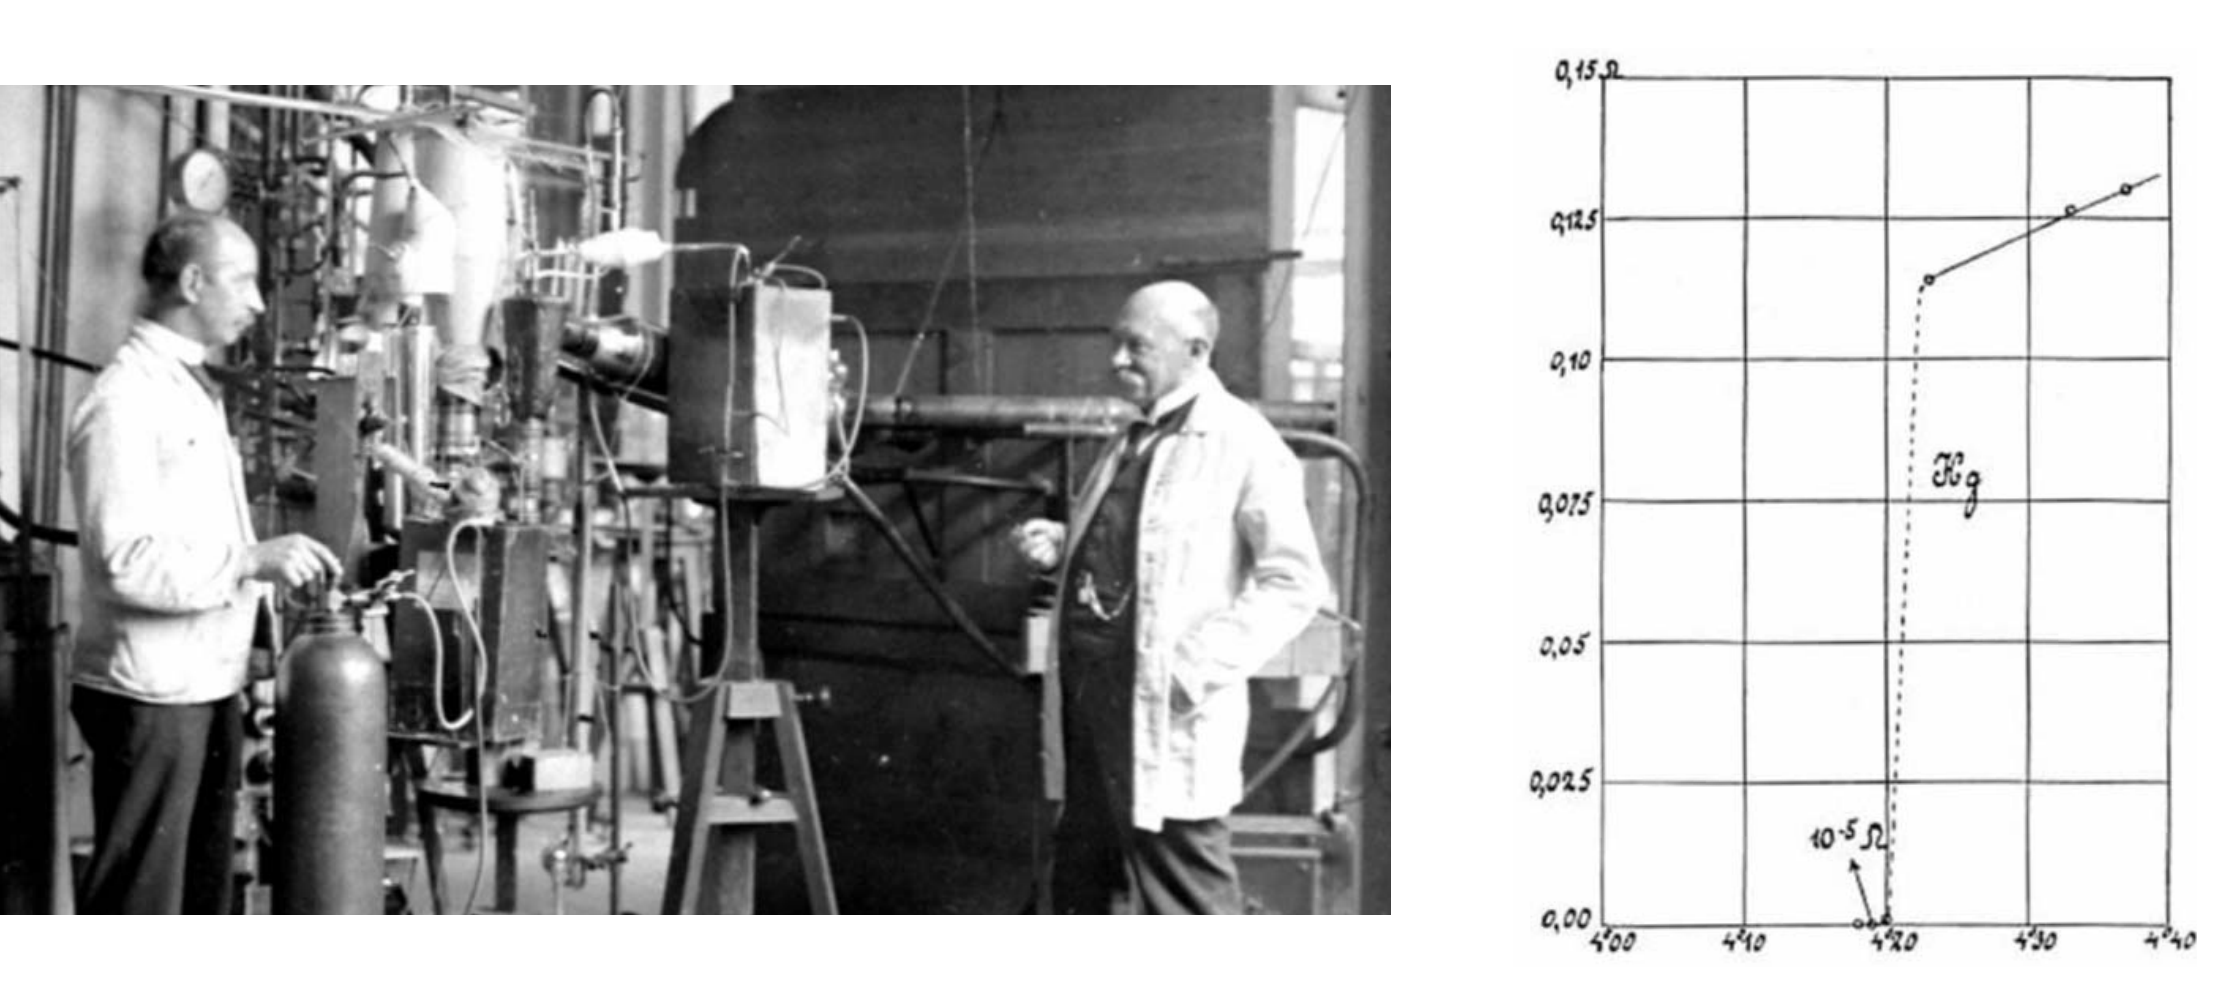
\includegraphics[width=\textwidth]{fig/intro/onnes.png}
    \caption{\textbf{Left}: Kammerling Onnes (right) and his chief engineer (left) in their cryogenics lab. \textbf{Right}: Resistivity as a function of temperature in elemental Lead. Both images from \cite{VanDelft2010}.}
    \label{fig:onnes}
\end{figure}

\begin{figure}
    \centering
    \missingfigure{Meissner effect}
    \caption{Meissner effect}
    \label{fig:meissner}
\end{figure}

Despite this remarkable experimental result, it would be 20 years for the next major milestone to appear. In 1933 the Meissner effect was discovered \cite{Meissner1933}, showing that superconducting materials would completely resist applied magnetic field by exhibiting perfect diamagnetism as sketched in figure \ref{fig:meissner}. In 1935 this effect was phenomenologically explained by the London equations, showing that the Meissner effect is due to superconducting currents on the surface of the material \cite{London1935}. From their relatively simple set of equations, an observable length scale known as the penetration depth was defined
%
\[ \lambda_\text{L} = \sqrt{\frac{m}{\mu_0 n q^2}} \, \]
%
where $\mu_0$ is the permeability of free space, $n$ the number concentration of the superconducting carriers, $m$ the electron mass and $q$ the electron charge. This length scale determines how an external magnetic field penetrates the superconductor through the relationship $B(x) = B(0) \exp (-x / \lambda)$. $\lambda$ is typically on the order of \SIrange{20}{100}{\nano\meter} \cite{Kittel2005}.

Another roughly 20 years would pass until Landau's work on phase transitions paved the way to understanding the superconducting phase transition as a thermodynamic quantity through the Ginzburg-Landau equations in 1950 \cite{Ginzburg2009}. I will not repeat the details here, but the idea is to make a polynomial expansion of the free energy as a function of a complex superconducting wavefunction $\psi$. As the material is cooled below $T_\text{c}$, $\psi$ `choses' a phase and breaks gauge symmetry, analogous to how a ferromagnet choses a common direction for the magnetic moment at the magnetic phase transition. This description predicts an new characteristic length scale of the superconductor called the \emph{coherence length} $\xi$ and recasts the penetration depth in terms of $\psi$:
%
\[ \xi = \sqrt{\frac{\hbar^2}{4m|\alpha|}} \qquad \lambda = \sqrt{\frac{m}{4\mu_0 e^2 \psi_0^2 }} \, , \]
%
where $\alpha$ is a phenomenological parameter of the polynomial expansion. The ratio of these parameters, $\kappa = \lambda / \xi$, are used to classify superconductors into type-I ($\kappa < 1 / \sqrt{2}$) and type-II ($\kappa > 1 / \sqrt{2}$). The significance of $\kappa > 1 / \sqrt{2}$ can be understood as a threshold where the surface tension between normal and superconducting phases becomes negative \cite{Abrikosov1957}. Intuitively, the coherence length $\xi$ defines the shortest length within which the superconducting carrier concentration are allowed to change considerably. For elemental metals $\xi$ can be on the nanometre to micrometre scale: \SI{1600}{\nano\meter} in Al and \SI{83}{\nano\meter} in Pb \cite{Kittel2005}. In the cuprates (which will be discussed in detail in the next section), $\xi$ is typically on the order of a few lattice spacings (\SI{1}{\nano\meter} in YBa$_2$Cu$_3$O$_{7-\delta}$ \cite{Tomimoto1999}).

Based on Ginzburg-Landau theory, \citeauthor{Abrikosov1957} predicted the existence of vortices in Type-II superconductors, which showed excellent agreement with the measured magnetization of several lead alloys \cite{Abrikosov1957}. These vortices can be pinned by defects and form a lattice that we have been able to image using modern day microscopy techniques (see e.g. \cite{Wells2015} for a recent example with beautiful real-space images). The experimental evidence piled up \cite{Doll1961, Deaver1961}, and it quickly became evident that Ginzburg-Landau theory is applicable to most known superconductors, including the cuprates and iron-based varieties.

Despite the descriptive power of Ginzburg-Landau theory, we are left with no recipe on how to construct, even theoretically, `better' superconductors. In order to manipulate material properties, it is necessary to understand the microscopic properties that lead to macroscopic behaviour (e.g. how phonons influence thermal properties or how magnetic exchange influence magnetic properties. Inspired by Ginzburg-Landau theory, rapid progress towards a microscopic theory was being made in the mid 1950s, culminating in the famous BCS theory formulated by Bardeen, Cooper and Schrieffer \cite{Bardeen1957}. 

BCS theory is based on the assumption that an attractive interaction between electrons at the Fermi level can result in so-called `cooper-pairs', a bosonic quasi-particle consisting of an electron pair of opposite momentum and spin. The bosonic nature of this quasi-particle can, at low temperatures, result in a Bose-Einstein condensate where a large fraction of these electron pairs occupy the lowest energy quantum state. This microscopic theory of superconductivity made several testable predictions, such as the appearance of an energy gap with a temperature-dependent width $\Delta(T)$ in the electronic density of states related to the critical temperature through the relationship
%
\[ 2\Delta(T=0) = 3.5 k_\text{B} T_\text{c} \, , \]
%
where $k_\text{B}$ is the Boltzmann constant. A few years later electron tunnelling experiments confirmed this prediction with reasonable accuracy \cite{Giaever1960, Giaever1960a}. Additionally, \citeauthor{Josephson1962} predicted that superconducting currents could tunnel across an insulating a barrier \cite{Josephson1962}, experimentally verified a few years later \cite{Jaklevic1965}.

While BCS theory predicts an attractive interaction between electrons, the original paper \cite{Bardeen1957} makes no assumption about the nature of this interaction. Some experiments, performed a few years prior, showed that $T_\text{c}$ of Hg$^{198}$ was higher when compared to that of natural Hg (avg. atomic weight of 200.6) \cite{Maxwell1950, Reynolds1950}. Since the chemistry of these materials can be assumed identical, this experiment suggests a positive correlation between phonon frequencies and $T_\text{c}$, since lighter elements have more energetic vibrations. Assuming an attractive potential due to lattice vibrations, BCS theory could relate the attractive interaction to phonon frequencies and predict a relative relationship between isotopic mass and critical temperature \cite{DeLaunay1954}:
%
\[ T_\text{c} \propto \frac{1}{\sqrt{m_\text{ion}}} \, , \]
%
where $m_\text{ion}$ is the isotopic mass of the constituent ionic species. With BCS theory, superconductivity in many elemental metals were believed to be `solved' with the identification of phonon-mediated superconductivity. Unfortunately, this discovery also set a \emph{practical} upper limit on $T_\text{c}$. In order to increase phonon frequencies, and thus critical temperatures, we need materials with low mass atomic species, while still being crystalline. At ambient pressure this practical upper limit is often quoted to be around \SI{30}{\kelvin}. A good demonstration of this principle is actually a counter-example where researchers were able to reach a critical temperature of $T_\text{c} = \SI{200}{\kelvin}$ by applying a pressure of \SI{155}{\giga\pascal} to H$_2$S \cite{Drozdov2015}. This material contains the light atomic species we require, but cannot crystallize at ambient pressures so we can only reach high critical temperatures under extreme conditions. A different example is the highly unusual case of MgB$_2$, where coincidences add up to an unusually high electron-phonon coupling resulting in a critical temperature of $T_\text{c} = \SI{39}{\kelvin}$ \cite{Nagamatsu2001}.

While this thesis has nothing to do with BCS superconductors and, in principle, could have been written without ever mentioning them, I believe that the history of conventional superconductivity emphasises exactly what is desired from a `solution' to high-temperature superconductivity. It is also a fascinating story due to the fact that the tools to solve the problem were not even close to being developed when the phenomenon was discovered. It took roughly 50 years for a satisfying conclusion and we have only been working on the cuprates for roughly 30 years. 

\section{Cuprates}
With this brief introduction to superconductivity, I will proceed with an introduction to cuprate superconductivity. While the previous section was at least moderately complete, it is difficult to capture an unbiased view of cuprate research. As such, the following will be somewhat narrowly focussed. While this is a reasonable choice for this introduction, it is important to realize just how massive the field is and how impossible it is to know every last detail. That being said, I have thoroughly enjoyed exploring the vast literature and I will recommend anyone reading this to do the same.

Before we begin, I want to get some of the nomenclature out of the way. As the title of this thesis suggest, I am working on the so-called `high-temperature superconductors'. This definition essentially only concerns itself with the value of the critical temperature (usually above the `BCS-limit' of \SI{30}{\kelvin}), without saying anything about other physical properties. On the other hand Type-I and Type-II, as seen in the previous section, are rigidly defined with respect to their properties as defined through Ginzburg-Landau Theory. Finally, `conventional superconductors' are those that can be microscopically described with BCS theory, while 'unconventional superconductors' cannot. While cuprates are relatively simple crystals, most of them have a variety of names and abbreviations attached to them. Table \ref{tab:cuprates} lists the most important ones along with their critical temperatures and a few other physical properties.

\begin{table}
    \caption{list of cuprates}
    \label{tab:cuprates}
    \missingfigure{Table of cuprates, formulae, names, Tc, crystal structure}
\end{table}

\subsection{The discovery of LBCO}
Roughly 30 years after BSC theory, in 1986, Bednorz and M\"uller discovered a new type of superconductor while trying to manipulate the electronic properties of the anti-ferromagnetic insulator La$_2$CuO$_4$. By effectively removing a small number of electrons from the system by substitution of dopant species, they achieved a record $T_\text{c}$ of \SI{30}{\kelvin}. Shortly after, in 1987, the sister-compound YBa$_2$Cu$_3$O$_{7-\delta}$ was discovered, shattering previous records and finally achieving a critical temperature $T_\text{c} = \SI{93}{\kelvin}$ that could be reached using liquid nitrogen \cite{Wu1987}.

While the increased critical temperatures are remarkable on their own, it quickly became apparent that we were dealing with a completely new type of superconductivity which cannot be explained with BCS theory. The normal state ($T > T_\text{c}$) of cuprate superconductors is as, if not more, complex when compared to the superconducting state and the BCS assumption of being metallic in the normal state is generally not fulfilled. In addition, the BCS relationship between isotopic mass critical temperature ($T_\text{c} \propto m_\text{ion}^{-0.5}$) is not fulfilled when performing O$^{16}$/O$^{18}$ isotopic substitution \cite{Suryadijaya2005}.

Similar to semiconductors, the properties of the cuprates are dramatically changed with the introduction of dopant species. In general, we call the addition of electrons \emph{electron doping} and the removal of electrons \emph{hole doping}. In the original paper, La$_2$CuO$_4$ was hole-doped by exchanging La$^{3+}$ with Ba$^{2+}$. We define the amount of hole-doping ($n_\text{h}$) as the fraction of substituted atomic species per CuO$_2$ layer. The amount of electron doping ($n_\text{e}$) is defined similarly. In general, the undoped compounds $n_\text{h} = 0$ are antiferromagnetic insulators and you need a small amount of doping to make the materials superconducting. Too much (typically $n_\text{h} > 0.25$) and the materials become non-superconducting metals. 

The fact that we need finite amounts of doping in order to make cuprates superconducting, makes them inherently inhomogeneous materials. This inhomogeneity may or may not be important for cuprate superconductivity, but there is no denying that it exists. In fact, recent STM studies on Bi$_2$Sr$_2$CaCu$_2$O$_8+\delta$ have shown significant spatial inhomogeneities due to random distributions of defects \cite{Ruan2018}. If this inhomogeneity is relevant, it presents us with a great difficulty in producing models that can explain superconductivity; adding too much complexity can be detrimental to explanatory power (Occam's razor).

\subsection{Structure}
Cuprate superconductors are characterized by a layered structure where CuO$_2$ layers are separated by so-called charge reservoirs (or spacer layers). In general, the conventional Bravais lattice is either tetragonal or orthorhombic with the CuO$_2$ layers in the $a$-$b$ plane. A few examples of cuprate crystal structures is shown in figure \ref{fig:cuprate_family_structures}. The different structures are generally characterized by the number $n$ of subsequent CuO$_2$ layers. Interestingly, increasing $n$ generally improves the critical temperature $T_\text{c}$ up to $n = 3$. It has been suggested that the decrease at $n \geq 3$ could be due to the fact that the `inner' and `outer' CuO$_2$ layers cannot reach similar doping.

\begin{figure}
    \centering
    \missingfigure{selection of cuprate crystal structures, LSCO on the left}
    \caption[various cuprate structures]{various cuprate structures}
    \label{fig:cuprate_family_structures}
\end{figure}

Doping is performed either by substitution or addition of dopant species as indicated by figure \ref{fig:cuprate_family_structures}. Doping thus necessarily changes the lattice either due to a difference in ionic radii of a substitutional dopant or a strain in the lattice because of an interstitial species. In the case of substitutional doping of La$_2$CuO$_4$, the structural and electronic properties vary wildly (as we shall see in section \ref{sec:lsco}) depending on the dopant species (Ba, Sr).

Different members of the cuprate family have their own structural peculiarities. In single-layer LSCO, many structural properties are linked to the CuO$_6$ octahedra not present in structures with $n \geq 2$ and In YBCO, Cu-O chains form along the crystallographic $b$-axis. Despite these specific structural properties of the various cuprates, they are all equipped with square-planer CuO$_2$ planes and have remarkably similar (electronic) phase diagrams.

\subsection{Phase diagram}
A general phase diagram for the cuprates is shown in figure \ref{fig:cuprate_phase_keimer} illustrating the many macroscopic and microscopic phases in the cuprates as a function of temperature and doping. First, figure \ref{fig:cuprate_phase_keimer} (left) shows an unexpected asymmetry between hole and electron-doping. Since cuprates are superconducting for a wider range of doping on the hole-doped side, most research focusses on this side of the phase diagram\todo{Other arguments? More discussion of the assymetry?}. Second, as shown in figure \ref{fig:cuprate_phase_keimer} (right), cuprates are only superconducting for a narrow range of hole doping typically between $n_h = 0.05$ and $n_h = 0.25$ with a maximum around $n_h = 0.15$. This region is known as the `superconducting dome'. 

\begin{figure}
    \centering
    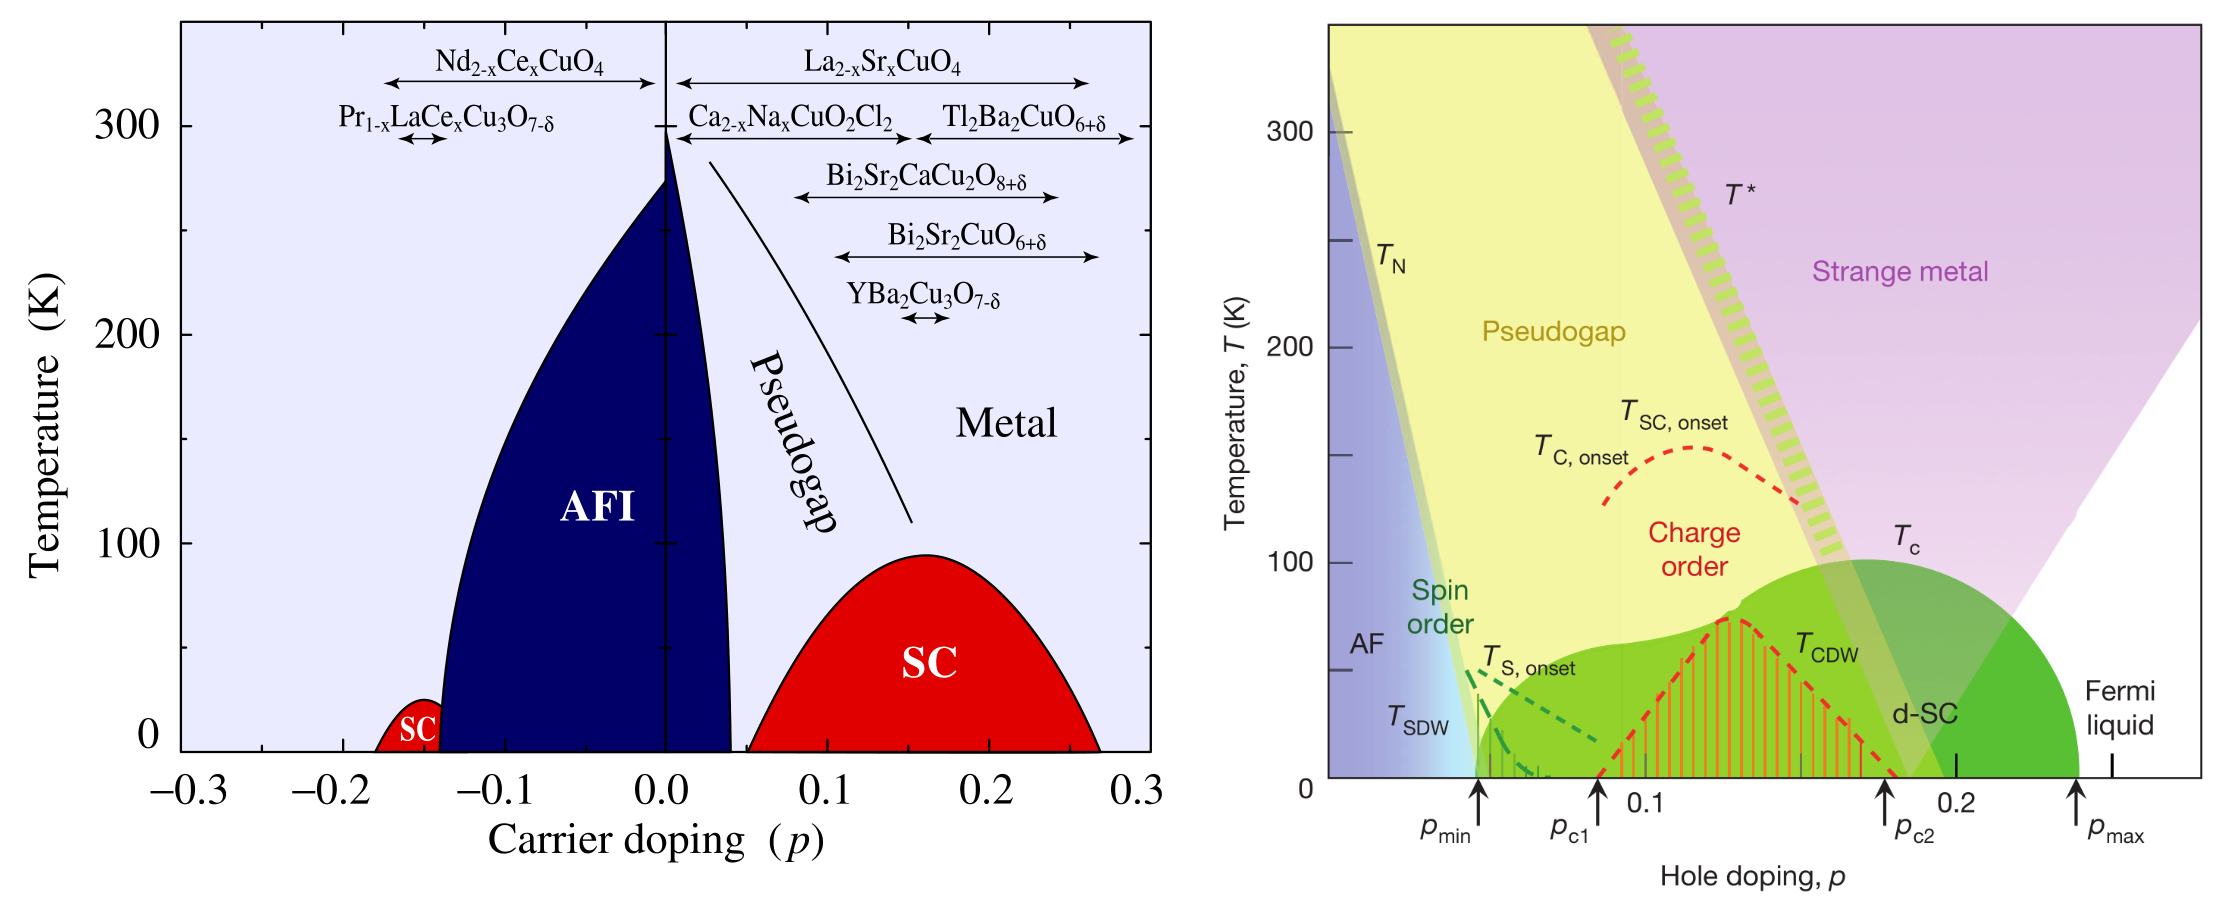
\includegraphics[width=\textwidth]{fig/intro/keimer.png}
    \caption[cuprate phase diagrams]{\textbf{Left:} Generalized phase cuprate phase diagram for selected electron- and hole-doped materials, emphasizing the asymmetry between the two sides of the phase diagram. From \cite{Peets2007}. \textbf{Right:} Generalized phase diagram for the hole-doped side annotated with microscopic ordering phenomena. From \cite{Keimer2015}.}
    \label{fig:cuprate_phase_keimer}
\end{figure}

I emphasize here the very different states of matter at the boundaries of the superconducting dome at $T=0$: Over-doped cuprates are typically metals while underdoped cuprates are magnetic insulators. In some sense, superconductivity is optimized in a region between localized (magnet) and itinerant (metal) behaviour -- a region also containing poorly understood normal state ($T > T_\text{c}$) behaviour such as the Pseudogap and strange metal phase.

The Pseudogap is a curious phenomena first observed in NMR measurements of YBCO \cite{Alloul1989} and later on in the $c$-axis resistivity \cite{Homes1993} and specific heat \cite{Loram1993}. The name comes from the fact that, by now, it is generally associated with the opening of a gap in the electronic density of states (see below). The difficulty in finding a microscopic origin of the phase transition at the Pseudogap temperature $T^*$ has attracted as much attention as the superconducting transition itself. Many researchers believe that the key to understanding the superconducting transition is directly related to the Pseudogap. One idea is that of `pre-formed pairs', where Cooper pairs start forming at $T^*$, but the macroscopic superconducting state fails to settle between $T^*$ and $T_\text{c}$ due to incoherent fluctuations in the phase of the pairing field ($\psi$ in Ginzburg-Landau theory) \cite{Emery1995, Curty2003}.\todo{maybe remove this last bit, too technical}

The strange metal phase is possibly the least understood part of the cuprate phase diagram \cite{Keimer2015}. A `strange' metal is essentially a phase of matter where the theory of `normal' metals (fermi liquids) breaks down and is a phenomenon seen in a number of correlated electron systems, not just the cuprates. A significant indicator of this behaviour is a linear temperature-dependence of resistivity (see e.g. \cite{Martin1990} for a cuprate example), where a normal fermi liquid varies as $T^2$ at low temperatures. A recent study even suggests that linear-in-$T$ resistivity in the cuprates is a generic property related to a universal scattering rate \cite{Legros2018}.

By outlining the the phase diagram in this way, I intend to illustrate both the difficulty of solving the cuprate problem and the many experimental methods and theoretical tools necessary to investigate the various features of this complex phase diagram. Until now, apart from crystallographic information, we have mainly considered \emph{macroscopic} behaviour through bulk measurements such as resistivity, specific heat, optical band gap or magnetic susceptibility. We now turn to a brief overview of \emph{microscopic} behaviour, starting with momentum-resolved measurements of the fermi surface.

\subsection{Fermi Surface}
Angle-Resolved Photoemission Spectroscopy (ARPES) is a method in X-ray spectroscopy that directly probes the electronic band structure of materials. This method has been extremely important in strongly correlated electron systems in general and has a rich history with the cuprates (see the extensive review by \citeauthor{Damascelli2003} \cite{Damascelli2003}, which also serves as a good introduction to the experimental method).

\subsection{Microscopic correlations}
The primary method for investigations in this thesis is inelastic neutron scattering (INS), which will be covered extensively in chapter \ref{ch:method}. For now, we just briefly state some of the things that can be measured by this and related methods.

\section{Lanthanum Based Cuprates}\label{sec:lsco}
In this section, we look more closely at the Lanthanum based cuprates. These are variants of the material discovered by Bednorz and M\"uller all based on the La$_2$CuO$_4$ parent compound (leftmost compound on figure \ref{fig:cuprate_family_structures}). Sometimes known as `La214' or with specific acronyms depending on the dopant species, these materials are single-layer cuprates with a relatively simple crystal structure and a maximum critical temperature $T_\text{c} \approx \SI{40}{\kelvin}$.

Since this thesis is focussed on specific structural aspects and phonon dynamics, this `relatively' simple crystal structure is a particularly strong point for us. Since we want to model the full 3-dimensional structure using computationally heavy simulation methods, it is advantageous to consider the simplest system possible. In addition, since the lanthanum cuprates were the first so-called 'high-temperature superconductors` to be discovered, there is a massive amount of literature on which to build our ideas from.  

In the phase diagram presented in figure \ref{fig:cuprate_phase_keimer}, a few of the many phenomena in the cuprates were indicated. In this section we will discuss these phenomena specifically in the context of lanthanum cuprates and relate them to other compounds where applicable. 


\begin{figure}
    \centering
    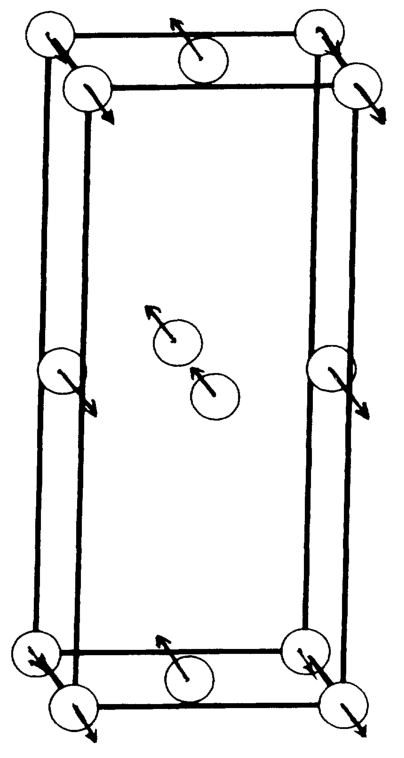
\includegraphics[width=0.3\textwidth]{fig/lsco/lsco_afm.png}
    \caption[AFM structure of LSCO]{AFM structure of LSCO}
    \label{fig:lsco_afm}
\end{figure}

\section{LSCO+O}

\section{Thesis objectives}

%\chapter{Properties of LSCO}
\section{Structure}
\section{Spin Dynamics}
\section{Lattice Dynamics}
\newcommand{\jp}{j^\prime}
\newcommand{\jpp}{j^{\prime\prime}}
\newcommand{\lp}{l^\prime}
\newcommand{\lpp}{l^{\prime\prime}}
\newcommand{\fc}{\bm{\Phi}\genfrac{(}{)}{0pt}{}{j \jp}{l \lp}}
\newcommand{\fczero}{\bm{\Phi}\genfrac{(}{)}{0pt}{}{j \jp}{0 \lp}}
\newcommand{\fcb}{\bm{\Theta}\genfrac{(}{)}{0pt}{}{j \jp}{l \lp}}
\newcommand{\fcbpp}{\bm{\Theta}\genfrac{(}{)}{0pt}{}{j \jpp}{l \lpp}}
\newcommand{\fcbf}{-\bm{\Theta}\genfrac{(}{)}{0pt}{}{j \jp}{l \lp} + \delta_{j,\jp} \delta_{l,\lp} \sum_{\jpp, \lpp}  \bm{\Theta}\genfrac{(}{)}{0pt}{}{j \jpp}{l \lpp} }
\newcommand*\tageq{\refstepcounter{equation}\tag{\theequation}}

\chapter{Simulation methods}

\section{Density Functional Theory}\label{sec:dft}

\subsection{The many-body wavefunction}
In electronic structure calculations we are ultimately interested in the many-body wavefunction

\[ \Psi(\bm{r}_1,\bm{r}_2,\dots, \bm{r}_n; \bm{R}_1, \bm{R}_2, \dots , \bm{R}_N) \]

\noindent where $\bm{r}_i$ are electron coordinates and $\bm{R}_i$ are nuclear coordinates. Imagine that we want to calculate this object for a small molecule such as Benzene (C$_6$H$_6$) containing 12 nuclei and 42 electrons. This wavefunction exists in $42\cdot3-6 = 156$ dimensional cartesian space! If we want to store this object on a computer with a modest precision of 10 grid points per coordinate, it would require $10^{156}$ complex numbers or $64 \cdot 10^{156}$ bits (assuming single-precision floating points numbers of 32 bits). Lloyd2000 estimated the total number of bits available for computation in the observable universe to be $10^{90}$ (Lloyd2000). Even with the entire universe at our disposal this object is completely unmanageable. This exercise also emphasizes the potential of Quantum Computers. For this reason, we fix the ionic positions and assume that the many-body wavefunction can be written as a product of single-electron wavefunctions (orbitals):

\[ \Psi(\bm{r}_1,\bm{r}_2,\dots, \bm{r}_n; \bm{R}_1, \bm{R}_2, \dots , \bm{R}_N) \longrightarrow \phi(\bm{r}_1)\phi(\bm{r}_2)\dots\phi(\bm{r}_n) \]

\subsection{The Kohn-Sham equations}

\subsection{The Hellman-Feynman theorem and molecular forces}

\subsection{DFT+U}

\section{Phonon calculation formalism}
In most textbooks (e.g. Kittel \cite{Kittel2005}), phonon calculations are exemplified by simple models in one dimension consisting of only one or two inequivalent atoms. While these models are useful for providing basic results of lattice dynamical models, the extension to realistic models requires some level of abstraction in order to be useful. In particular, it is essential to cast the problem in terms of linear algebra. In this section, I will start from the (somewhat abstract) formalism used in practice and work backwards towards a physical understanding. While software such as PHONON \cite{Parlinski1997} and Phonopy \cite{Togo2015} can be used without prior knowledge of the formalism, it is always useful to have some insights about our frequently used 'black boxes`. In order to calculate the phonon spectrum for a given system in the harmonic approximation, we require the following objects:

\begin{enumerate}
	\item Primitive unit cell and fractional atomic coordinates
	\item Symmetry operations
	\item The mass of each atomic species
	\item The force constants
\end{enumerate}

Items 1-3 are familiar to most condensed matter physicists and can usually be found in various databases. The force constants, on the other hand, contains information about interatomic forces and is not directly obtainable from experiment. For this reason, phonon calculations requires some modelling either through semi-empirical or ab-initio methods. In the following I will attempt to explain what the force constants represents and how we use them to get phonon band structures.

\subsection{Theory}

We start completely generally in one dimension with an arbitrary number of unit cells containing an arbitrary number of atomic species at equilibrium. Displacements from equilibrium positions are denoted $u(jl)$, where $l$ is the unit cell index and $j \in \{1,\dots,n\}$ is the atomic index. If we consider the displacements $u$ to be small, the total energy of our system can be expressed as a Taylor series

\[ E^\text{tot} = E_0 + \sum_{l}\sum_{j} \left. \frac{\partial E}{\partial u(jl)} \right\rvert_{r_{lj}}  + \frac{1}{2} \sum_{l,\lp} \sum_{j,\jp} u(jl) \left. \frac{\partial ^2 E}{\partial u(jl) \partial u(\jp \lp)} \right\rvert_{r_{lj}, r_{\lp \jp}} u(\jp \lp) + \dots \, , \]

\noindent where $r_{lj}$ is the equilibrium position of atom $j$ in unit cell $l$. The main approximation in phonon calculations is the so-called \emph{harmonic approximation} which ignores terms with power greater than 2 in the series. Higher-order contributions are denoted \emph{anharmonic} terms and can become important at higher temperatures (phase transitions, thermal conductivity, thermal expansion). The fact that our system is in equilibrium can be stated succinctly as

\[ \frac{\partial E}{\partial u(jl)} = 0 \, , \]

\noindent for all values of $j$ and $l$. Physically these assumptions together correspond to atoms being at rest in a parabolic (harmonic) potential. Since we are interested in  dynamics, it is convenient to consider the \emph{harmonic energy} $E$ of the system

\begin{equation}
E = E^\text{tot} - E_0 = \frac{1}{2} \sum_{l,\lp} \sum_{j,\jp} u(jl) \left. \frac{\partial ^2 E}{\partial u(jl) \partial u(\jp \lp)} \right\rvert_{r_{lj}, r_{\lp \jp}} u(\jp \lp) \label{eq:eharm}
\end{equation}

\noindent If we set $j=\jp$ and $l=\lp$, we see that the harmonic energy of a single atom has the familiar form of a harmonic oscillator $E=\frac{1}{2}Ku^2$, where $K$ is the spring constant. We define

\[ \left. \frac{\partial ^2 E}{\partial u(jl) \partial u(\jp \lp)} \right\rvert_{r_{lj}, r_{\lp \jp}} = \fc = \fcbf \]

\noindent where $\bm{\Phi}$ is the called the \emph{force constant} with respect to total energy and $\bm{\Theta}$ is the force constant with respect to bond energy. We can now write the harmonic energy as

\begin{align*}
E &= \frac{1}{2} \sum_{l,\lp} \sum_{j,\jp} u(jl) \fc u(\jp \lp) \tageq\label{eq:total_energy} \\
&= \frac{1}{2} \sum_{l,\lp} \sum_{j,\jp} u(jl) \left( \fcbf \right) u(\jp \lp) \\
&= \frac{1}{2} \sum_{l,\lp} \sum_{j,\jp} \left( - \fcb u(jl)u(\jp,\lp) + \fcb u(jl)^2 \right) \\
&= \frac{1}{2} \sum_{l,\lp} \sum_{j,\jp} \left( - \fcb u(jl)u(\jp,\lp) +\frac{1}{2} \fcb \left( u(jl)^2 + u(\jp, \lp)^2 \right) \right) \\
&= \frac{1}{4} \sum_{l,\lp} \sum_{j,\jp} \fcb \left[ -2u(jl)u(\jp,\lp) + u(jl)^2 + u(\jp,\lp)^2 \right] \\
&= \frac{1}{4} \sum_{l,\lp} \sum_{j,\jp} \fcb \left[ u(jl) - u(\jp,\lp) \right]^2
\end{align*}

\begin{figure}
	\centering
	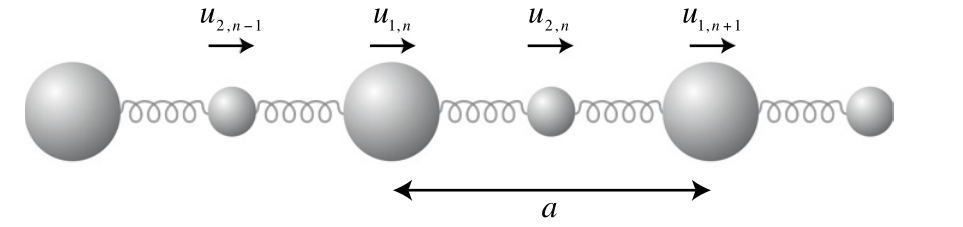
\includegraphics[width=0.9\textwidth]{fig/temp/diatomic.png}
	\caption[diatomic chain]{Diatomic chain. \todo[inline]{Make new figure. Use $l$ as unit cell index for consistency with the notation.}}
	\label{fig:diatomic}
\end{figure}

\noindent and it becomes evident that the harmonic energy can be described with respect to atoms or bonds in mathematically equivalent ways. Since the bond-centered description does not include individual atomic displacements, it is necessary to add a self-term to $\bm{\Theta}$. As a visual aid to these index-heavy equations, Figure \ref{fig:diatomic} illustrates the one-dimensional diatomic chain, which is often used in introductory texts. If we consider only nearest-neighbour interactions and identical springs, the bond-centered harmonic energy can be written

\begin{align*}
E &= \frac{1}{4} \bm{\Theta} \sum_l 2 \left[ u(1,l) - u(2,l) \right]^2 + \frac{1}{4} \bm{\Theta} \sum_n 2 \left[ u(2,l) - u(1,l+1) \right]^2 \\
&= \frac{1}{2} \bm{\Theta} \sum_l \left[ u(1,l) - u(2,l) \right]^2 + \frac{1}{2} \bm{\Theta} \sum_n \left[ u(2,l) - u(1,l+1) \right]^2
\end{align*}

\noindent where the factor of 2 comes from double-counting. The purpose of this example is to show that the (somewhat abstract) harmonic energy in equation \eqref{eq:eharm} is equivalent to our intuitive understanding of coupled harmonic oscillators. With this in mind, we can return to the matter at hand and write the equation of motion for an atom $j$ in cell $l$ through Newtons second law $F=ma$:

\[ m_j \ddot{u}(jl, t) = - \frac{\partial E}{\partial u(jl)} = - \sum_{\lp} \sum_{\jp} \fc u(\jp \lp, t) \, , \]

\noindent where $m_j$ is the atomic mass of atom $j$\todo{Where does the factor 2 come from when taking the derivative?!?}. Solutions to this equation is given as a sum of travelling harmonic waves with wave vectors $q$ and band indices $\nu \in \{1,\dots , n \}$

\[ u(jl,t) = \sum_{q,\nu} \tilde{u}(j,q,\nu) \exp (iqr(jl)) \exp(-i \omega(q,\nu) t) \, \]

\noindent where $\omega(q,\nu)$ is the frequency, $r(jl)$ is the position of atom $j$ in cell $l$ and  is the frequency and the complex number $\tilde{u}$ is called the \emph{displacement vector}. If we insert these solutions into the equations of motion and just consider one band at one wave vector we obtain

\begin{align*}
m_j \omega(q,\nu)^2 \tilde{u}(j,q,\nu) \exp(ikr(jl)) &= - \sum_{\lp} \sum_{\jp} \fc \tilde{u}(\jp,q,\nu) \exp (ikr(\jp\lp)) \\
m_j \omega(q,\nu)^2 \tilde{u}(j,q,\nu) & = - \sum_{\lp} \sum_{\jp} \fc \tilde{u}(\jp,q,\nu) \exp (ik[r(\jp\lp) - r(jl)]) \\
m_j \omega(q,\nu)^2 \tilde{u}(j,q,\nu) & = - \sum_{\lp} \sum_{\jp} \fczero \tilde{u}(\jp,q,\nu) \exp (ik[r(\jp\lp) - r(j0)]) \tageq\label{eq:motion} \, ,
\end{align*}

\noindent where the last equality is simply a change of origin in order to follow the convention of most software. The full account of phonon frequencies $\omega$ and displacements $\tilde{u}$ can be found as a solutions to equation \eqref{eq:motion}. At a given $q$ and $\nu$, the equations are indexed by $j$ and we will have $n$ equations with $n$ unknowns with respect to $\tilde{u}(j,q,\nu)$, where $n$ is the number of atoms in the unit cell. In fact, equation \eqref{eq:motion} can be written as an eigenvalue equation:

\begin{equation}
\bm{D}(q) \cdot \bm{e}(q,\nu) = \omega(q,\nu)^2 \cdot \bm{e}(q,\nu) \, , \label{eq:dynmat}
\end{equation}

\noindent where 

\[ \bm{e}(q,\nu) = \begin{pmatrix}
\sqrt{m_1}\tilde{u}(1,q,\nu) \\
\sqrt{m_2}\tilde{u}(2,q,\nu) \\
\vdots \\
\sqrt{m_n}\tilde{u}(n,q,\nu)
\end{pmatrix} \]

\noindent and the elements of $\bm{D}(q)$ are given 

\begin{equation}
D(j\jp) = \frac{1}{\sqrt{m_j m_{\jp}}} \sum_{\lp} \fczero \exp (iq[r(\jp\lp) - r(j0)]) \, . \label{eq:dynmat_ij}
\end{equation}

\noindent $\bm{D}(q)$ is known as the dynamical matrix and can be constructed solely from force constants. Furthermore, equation \eqref{eq:dynmat_ij} reveals that the dynamical matrix is Hermitian so the eigenvalues $\omega(q,\nu)^2$ are real and the eigenvectors $\bm{e}(q, \nu)$ are orthonormal. In addition, the eigenvalues and eigenvectors are trivially obtained numerically (e.g. \texttt{numpy.linalg.eigh} in the Python numpy library). In order to get the full dispersion, this diagonalization is performed for each of the $n$ bands $\nu$ at the desired wave vectors in the first Brillouin Zone (FBZ). 

The extension to 3 dimensions is done by treating the Cartesian components separately and considering $\bm{q}$ and $\bm{r}$ as vectors. The eigenvector then becomes a column vector of $3n$ components 

\[ \bm{e}(\bm{q},\nu) = \begin{pmatrix}
\sqrt{m_1}\tilde{u}_x(1,\bm{q},\nu) \\
\sqrt{m_1}\tilde{u}_y(1,\bm{q},\nu) \\
\sqrt{m_1}\tilde{u}_z(1,\bm{q},\nu) \\
\sqrt{m_2}\tilde{u}_x(2,\bm{q},\nu) \\
\vdots \\
\sqrt{m_{n}}\tilde{u}_z(n,\bm{q},\nu)
\end{pmatrix} \, , \]

\noindent the number of bands increase to $3n$ and we get a $3n \times 3n$ dynamical matrix, where each component \eqref{eq:dynmat_ij} is a $3 \times 3$ block of the form

\[
\bm{D}(j\jp) = \begin{pmatrix}
D(j\jp)_{xx} & D(j\jp)_{xy} & D(j\jp)_{xz} \\
D(j\jp)_{yx} & D(j\jp)_{yy} & D(j\jp)_{yz} \\
D(j\jp)_{zx} & D(j\jp)_{zy} & D(j\jp)_{zz}
\end{pmatrix}
\]

\noindent where

\begin{equation}
D(j\jp)_{\alpha\beta} = \frac{1}{\sqrt{m_j m_{\jp}}} \sum_{\lp} \fczero _{\alpha\beta} \exp (i\bm{q}[\bm{r}(\jp\lp) - \bm{r}(j0)]) \label{eq:dynmat_ij2}
\end{equation}

\noindent While the path was somewhat involved, it is useful to take a step back and consider the consequences of our outlined formalism. Everything we need to know about our phonon system can be obtained from the dynamical matrix that, in turn,  is constructed from force constants through equation \eqref{eq:dynmat_ij2}. Finally, all of these objects can be constructed in computationally trivial way from force constants.

\subsection{Practical considerations}\label{sec:phononpractical}
At this point, it is useful to consider how we construct elements of the dynamical matrix in practice. Inspection of equation \eqref{eq:dynmat_ij2} contains a sum over all unit cells $\lp$ and is thus an infinite sum. On the other hand, it is reasonable to assume that the dominant force constants $\bm{\Phi}$ are short range. The compromise is to use a finite supercell such that the second derivatives involved in calculating force constants outside this cell are minimized. While the reasonable size of such a supercell obviously depends on the system and model, quantum contributions to the force constants generally vanish within a distance of roughly \SIrange{10}{15}{\angstrom} \todo{CRYSTAL website reference? Maybe something better}. If the force constants can be obtained analytically from a semi-empirical potential, calculation is computationally simple and we can use large supercells. However, since force constants are usually obtained from DFT, we are limited by computational resources and are usually restricted to supercells with a maximal interatomic distance of roughly \SI{5}{\angstrom} (e.g. a cubic system with $a=\SI{10}{\angstrom}$).

Since the number of force constants needed is at least equal to the size of the dynamical matrix, the number of calculations to perform is at least $3n \times 3n$. Even for a fairly small system such as LCO in the I4/mmm space group (HTT, $n=7$) the number of elements in the dynamical matrix is $(3\cdot 7)^2 = 441$. In the finite displacement method, each force constant is the result of a self-consistent DFT calculation, so the computational effort appears prohibitively expensive at first glance. For this reason we use a numerical fitting of symmetry inequivalent force constants (see section \ref{sec:forceDFT}). In the case of LCO in the I4/mmm space group the number of necessary displacements is reduced to only 7 (6 if we ignore magnetism), making the problem much more manageable.

\subsection{Phonon eigenvectors}
The phonon dispersion is contained within the eigenvalues $\omega (\bm{q},\nu)^2$. We can plot the bands $\nu$ along high-symmetry lines in the FBZ by carefully choosing the values of $\bm{q}$ where the dynamical matrix is diagonalized. Similarly, we can sample the dispersion in a dense $\bm{q}$-mesh in order to evaluate the phonon density of states. In addition, many thermodynamic properties can be calculated by only considering the eigenvalues.

The eigenvectors $\bm{e}(\bm{q}, \nu)$ are more subtle in nature. Each component of  $\bm{e}(\bm{q}, \nu)$ is a complex number that describes the wave amplitude and phase of one atomic species $j$ in one cartesian direction $\alpha$. In addition, the eigenvector is normalized and thus only describes relative atomic motion. In order to visualize the collective displacement due to a phonon mode $\nu$ at $\bm{q}$ we can displace all atoms $j$ in unit cells $l$ by

\begin{equation}
\Delta_{jl} = \frac{A}{\sqrt{m_j}} \text{Re} \left[ \exp (i\phi) \bm{e}_j(\bm{q}, \nu) \exp (i \, 2 \pi \, \bm{q} \cdot \bm{r}(jl) \right] \label{eq:displacements}
\end{equation}

\noindent where $\bm{e}_j(\bm{q}, \nu)$ is the $j$'th component of $\bm{e}(\bm{q}, \nu)$ and $A$ is an arbitrary amplitude. The phase $\phi$ describes periodic motion of atoms. An animation can be produced by varying $\phi$ between 0 and $2 \pi$.

In \texttt{Phonopy} the eigenvectors are always given with respect to the primitive unit cell and the 3 Cartesian components are along the basis vectors of this primitive unit cell. If we want to, for example, to visualize the bond-stretching mode in the HTT phase of LCO at $q=(\frac{1}{4},\frac{1}{4},0)$ in orthorhombic notation, we look at atoms in primitive unit cells with origin (0,0,0), (1,0,1), (2,0,2) and (3,0,3) using the eigenvectors at $q=(0.125,-0.125,0.125)$. For this specific mode, the movement of oxygen with fractional coordinates (0.5,0,0.5) dominates. The movement is exactly along the Cu-O bond and we can plot it in one dimension. Figure \ref{fig:bs-displacements} shows this phonon mode at the zone center, the zone boundary and halfway through the zone (where the giant phonon anomaly is observed).

\begin{figure}
	\centering
	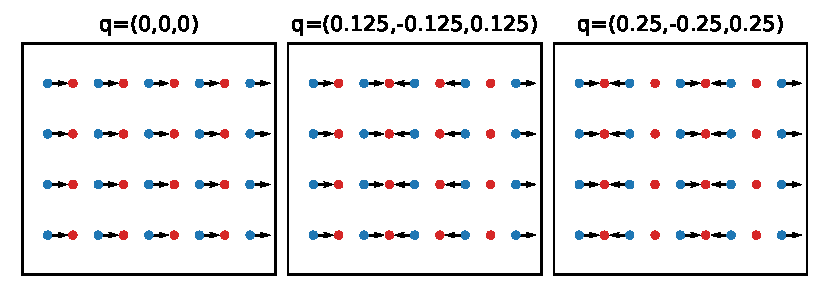
\includegraphics{fig/temp/bs-phonons.pdf}
	\caption[bond-stretching phonons visualized]{Cu-O bond stretching mode in LCO at three different values of $q$ referring to the primitive HTT (I4/mmm) unit cell. Blue markers are oxygen and red markers are copper. The phase is set to $\phi=\frac{3}{4}\pi$ in equation \ref{eq:displacements} in order to get displacement vectors of equal length.}
	\label{fig:bs-displacements}
\end{figure}

\subsection{Obtaining Force Constants from DFT}\label{sec:forceDFT}
Force constants from DFT are found in a surprisingly simple way. In the previous sections we defined the force constant with respect to total energy as

\[ \fc  _{\alpha \beta} = \frac{\partial ^2 E}{\partial u_\alpha (jl) \partial u_\beta (\jp \lp)} = - \frac{\partial F_\beta (\jp \lp)}{\partial u_\alpha (jl)} \]

\noindent where $F_\beta (\jp\lp)$ is the force on atom $(\jp \lp)$ in the direction $\beta$. Notice that everything is now labelled by a Cartesian direction and these directions are treated individually. In practice the Cartesian directions correspond to the unit cell vectors, but to reduce confusion we use the labels ($x,y,z$). We can approximate the derivative by performing a finite displacement $\Delta u_\alpha(jl)$ and simply taking the numerical derivative


\begin{equation}
\fc _{\alpha \beta} \approx - \frac{F_\beta (\jp \lp; \Delta u_\alpha (jl)) - F_\beta (\jp\lp)}{\Delta u_\alpha (jl)} \label{eq:finite}
\end{equation}


\noindent where $F_\beta (\jp\lp;\Delta u_\alpha (jl))$ is the force on atom $(\jp \lp)$ in the direction $\beta$ after performing the displacement $\Delta u_\alpha (jl)$. At equilibrium we assume $F_\beta (\jp \lp) = 0$ and we only need to calculate the forces due to a finite displacement. In ab-initio methods, there is no reason to assume a particular shape of the potential energy landscape and we can only expect the harmonic approximation to be valid for small finite displacements. For this reason, displacements have to be chosen large enough so that we are not subject to numerical noise and small enough to avoid anharmonic contributions. In \texttt{Phonopy} the default value is \SI{0.01}{\angstrom}, while \texttt{PHONON} uses \SI{0.03}{\angstrom}.

As mentioned in section \ref{sec:phononpractical}, we need a large number of force constants to construct the dynamical matrix, even when dealing with small systems. For this reason, a numerical fitting of forces and displacements, known as the Parlinski-Li-Kawazoe method \cite{Parlinski1997}, is used to find force constants. We notice that equation \eqref{eq:finite} can be written as a matrix equation for one pair of atoms $(jl)$ and $(\jp \lp)$:

\[ \bm{F}(\jp \lp) = -\bm{U}(jl) \bm{P} (jl;\jp \lp) \, , \]

\noindent where

\[ \bm{F}(\jp \lp) = (F_x \quad F_y \quad F_z) \, , \]

\[ \bm{U}(jl) = \left( \Delta u_x(jl) \quad \Delta u_y(jl) \quad \Delta u_z(jl) \right)  \]

\noindent and

\[ 
\bm{P} (jl;\jp \lp) = 	
\begin{pmatrix}
\Phi_{xx} & \Phi_{xy} & \Phi_{xz} \\
\Phi_{yx} & \Phi_{yy} & \Phi_{yz} \\
\Phi_{zx} & \Phi_{zy} & \Phi_{zz} 
\end{pmatrix}
\]

\noindent If we perform $m$ finite displacements, we get $m$ simultaneous equations for each pair of atoms:

\begin{equation*}
\begin{pmatrix} \bm{F}_1(\jp\lp) \\ \bm{F}_2(\jp\lp) \\ \vdots \\ \bm{F}_m(\jp\lp) \end{pmatrix} =
- \begin{pmatrix} \bm{U}_1(jl) \\ \bm{U}_2(jl) \\ \vdots \\ \bm{U}_m(jl) \end{pmatrix} \bm{P}(jl;\jp \lp) \, .
\end{equation*}

\noindent which can be solved by a Moore-Penrose pseudo-inverse matrix (in Numpy: \texttt{numpy.linalg.pinv}) given a sufficient number of displacements. Since $\bm{U}$ only depends on $(jl)$, we can build up the full force constant matrix by iterating this procedure over $(\jp \lp)$. The minimum number of displacements is equal to the number of non-equivalent atoms in the crystal primitive unit cell multiplied by a number of independent x,y,z coordinates in the site symmetry of a given atom \cite{Parlinski1997}. For this reason, software such as \texttt{Phonopy} and \texttt{PHONON} determines the primitive unit cell, the supercell expansion matrix and all the symmetry operations before generating displacements.

\section{Molecular Dynamics}
Temperature fluctuations in a closed system:

\[ \frac{\Delta T}{T} = \sqrt{\frac{2}{3N}} \quad \Rightarrow \quad \Delta T(T=\SI{300}{\kelvin}) = \SI{23.1}{\kelvin} \]

\noindent Nose-Hover algorithm:

\begin{align*}
v_i^\text{scaled} &= \frac{\bm{p}_i}{m_i} \\
\text{d}\bm{p}_i &= (\bm{F}_i - \zeta \bm{p}_i) \text{d}t \\
\text{d}\zeta &= \frac{1}{Q} \left( \sum_{i=1}^N \frac{|\bm{p_i}|^2}{m_i} - (3N+1)k_\text{B}T\right) \text{d}t
\end{align*}

\subsection{MD Observables}
It turns out [dove] that the phonon density of states can be found from the power spectrum of the mass-weighted velocity autocorrelation function (VACF). The VACF is, as the name implies, an expression of the correlation between velocites at different. In liquids, the VACF will rapidly decay to zero and in solids the VACF will fluctuate due to coherent vibrations around equilibrium positions. The VACF for a single atomic species $\alpha$ is defined as

\[ C_\alpha(t) = \frac{1}{3} \langle \bm{v}_\alpha(t_0) \cdot \bm{v}_\alpha(t) \rangle \]

\noindent By invoking ergodicity, the ensemble average can be replaced with a time average with respect to $t_0$.

\[ C_\alpha(t) = \frac{1}{3} \frac{1}{T-t} \sum_{t_0=0}^{T-t} \bm{v}_\alpha(t_0) \cdot \bm{v}_\alpha(t_0 + t) = \frac{1}{3} \frac{1}{T-t} \sum_{t_0=0}^{T-t} \sum_{\beta=x,y,z} v_{\alpha\beta}(t_0) v_{\alpha\beta}(t_0 + t) \]

\noindent where $T$ is the total simulation time and $v_{\alpha\beta}$ is the velocity of atom $\alpha$ in direction $\beta$. The total VACF is defined as

\[ C(t) = \sum_\alpha w_\alpha C_\alpha(t) \]

\noindent where $w_\alpha$ is a weight depending on the atomic species. To get the mass-weighted VACF $w_\alpha$ is equal to the atomic weight of species $\alpha$.


\chapter{Experimental Methods}
\section{Neutron Scattering}
\section{X-ray spectroscopy}
\chapter{Simulation}

\begin{framed}
	\begin{itemize}
		\item An independent chapter on the structural phases of LSCO
		\item Software details
		\item Coordinate systems (reminder of HTT/LTO/LTT/LTLO)
		\item Convergence tests (Benchmarking)
		\item Electronic bands (Metal/AFM)
		\item Geometry optimization
		\item Phonon bands (PBESol seems to be neccesary)
		\item Molecular dynamics of defect Structures
		\item Validation against experiment.
		\item Discussion/conclusion
	\end{itemize}	
\end{framed}

In this chapter, results from ab-initio simulations are presented independent of experimental data. It turns out that a careful investigation of various phases of LSCO+O presents us with valuable clues regarding the average and local structure. While DFT is unable to capture the strongly correlated nature of the cuprates, it turns out to be a reasonable description with regards to intermolecular forces. The subsequent strategy is to carefully validate our simulations and establish a `one-electron baseline' for the studied systems. Experimental deviations from this baseline can then be analysed for clues possibly pertaining to superconductivity or other phenomena not captured at the DFT level of theory.

One example of such a deviation is shown in Chapter \ref{ch:anomaly}, where we can detect potentially interesting physics by following how a certain phonon mode diverges from our otherwise robust simulation results. In this chapter we perform DFT simulations based on the La$_2$CuO$_4$ parent compound across three structural and two electronic phases, all of which have been observed experimentally in the lanthanum-based cuprates. We then calculate phonons within the `Frozen-Phonon' approach and obtain the neutron-weighted phonon band structure. Since the computational requirements of phonon calculations are heavily influenced by symmetries, we do not consider defects such as interstitials in this chapter as this would make the computational effort unmanageable. To understand the dynamics due to dopant species, molecular dynamics simulations based on the results of this chapter are presented in Chapter \ref{ch:md}.

\section{Computational Details}
The theory and principles behind Density Functional Theory (DFT) is presented in chapter \ref{ch:method}, section \ref{sec:dft}. DFT simulations in this thesis are performed using the Vienna Ab-Initio Simulation Package (VASP) \cite{Kresse1993a, Kresse1994, Kresse1996, Kresse1996a} using Projector Augmented-Wave Pseudopotentials (PAW) \cite{Blochl1994a, Kresse1999} to describe the atomic wavefunctions. While ab-initio loosely translates to `from the beginning', There are several choices to be made with regards to computational parameters. First, we need to define the pseudo-potentials that describes the valence electrons of each atomic species in our system. For L(S)CO(+O), the relevant pseudo-potentials are listed in Table \ref{tab:vasp_pseudo} along with their electronic configuration. For both La and O we used the recommended potentials, while for Cu we used a more accurate version where all 6 3p electrons are included (\verb|_pv| is short for `p in valence'). The reason for this is simply because it was difficult to have the simulations converge with the standard potential -- not because we necessarily believe that the Cu 3p states are important for the chemistry of our system. To run a simulation in VASP, or in any DFT software, the following information (files) is required:

\begin{itemize}
	\item Crystal lattice and atomic coordinates (\texttt{POSCAR})
	\item Pseudopotential configuration (\texttt{POTCAR})
	\item $k$-point mesh (\texttt{KPOINTS})
	\item Computational parameters (\texttt{INCAR})
\end{itemize}

\begin{table}[b]
	\centering
	\begin{tabular}{@{}llll@{}}
	\toprule
	 & Z & Core (\# electrons) & Valence (\# electrons)                        \\ \midrule
	\texttt{La} & 57 & 1s$^2$2s$^2$2p$^6$3s$^2$3p$^6$3d$^{10}$4s$^2$4p$^6$4d$^{10}$ (46) & 5s$^2$5p$^6$5d$^1$6s$^2$ (11) \\
	\texttt{Sr\_sv} & 38 & 1s$^2$2s$^2$2p$^6$3s$^2$3p$^6$3d$^{10}$ (28) & 4s$^2$4p$^6$5s$^2$ (10) \\
	\texttt{Cu\_pv} & 29 & 1s$^2$2s$^2$2p$^6$3s$^2$ (12) & 3p$^6$3d$^{10}$4s$^1$ (17)      \\
	\texttt{O} & 8 & 1s$^2$ (2) & 2s$^2$2p$^4$ (6) \\ \bottomrule
	\end{tabular}
	\caption[VASP Pseudopotentials]{PAW psedopotenial electronic configuration used in VASP calculations. While lanthanum is typically placed in the f-block on periodic tables it's electronic configuration has no f-electrons. This is fortunate since DFT famously struggles with highly localized ortbitals.}
	\label{tab:vasp_pseudo}
\end{table}	

The choice of crystal lattice and atomic positions are typically taken from experiment, but it is important to realize that the simulation might not `agree' completely. This is especially important if we want to calculate phonons through the evaluation of forces due to displacements away from equilibrium positions. The pseudopotentials configuration is usually taken from a database since the generation of consistent, transferable potentials is a difficult, time-consuming task. In fact, the main selling point of VASP is their high-quality pseudopotentials. The $k$-point mesh defines the number of $k$-points where the wavefunctions and density is evaluated and has a huge impact on computational effort (going from e.g. a $2 \times 2 \times 2$ grid to a $4 \times 4 \times 4$ takes 8 times as many evaluations). Luckily, the amount of $k$-points needed for an accurate calculation usually converges rapidly and we often check this convergence explicitly. Since the density of the k-point mesh depends on the system size, it is common to state the $k$-point density which is defined as the number of $k$-points per reciprocal atom (or simply \#kpoints $\times$ \#atoms).

Finally, there is a large number of computational parameters that can be tweaked depending on the desired type of calculation. The VASP \texttt{INCAR} file has more than 300 optional tags \cite{zotero-1437}, but usually only a few needs to be tweaked depending on the desired type of simulation. For the simulations performed in this thesis the following keywords are important:

\begin{itemize}
	\item \texttt{ENCUT}: The plane-wave cut-off and thus the size of the basis set. Usually the default performs well, but for accurate forces, which are needed for phonons, this needs to be increased.
	\item \texttt{EDIFF}: The threshold for the the self-consistent cycle to terminate. For accurate forces this needs to be increased.
	\item \texttt{PREC}: A tag that defines the `precision' by setting new defaults for certain parameters. I generally increase this to `Accurate' for all simulations. `Normal' is the default.
	\item \texttt{LREAL}: A PAW pseudopotential specific tag which determines if a certain evaluation is performed in real or reciprocal space. This operation is faster in real space, but at the cost of accuracy. For phonons we want to perform the operation in reciprocal space.
	\item \texttt{GGA}: Sets the exchange-correlation functional (see section \ref{sec:dft}). Usually the default (PBE) is a good starting point, but experimentation is encouraged!
	\item \texttt{ISPIN} and \texttt{MAGMOM}: Turns on a spin-polarized calculation.
	\item \texttt{IBRION}: How and when to update the ionic positions. This can be used to perform molecular dynamics and structural optimizations in different ways.
	\item \texttt{ISMEAR} and \texttt{SIGMA}: A tag that controls `fermi surface smearing', which is important for metallic systems where we need to evaluate a discontinuous function at the fermi level due to partial occupancies. This can be done in several ways, and it is usually good practice to test the convergence and performance of these methods.
	\item \texttt{LDAU}: Switches on LDA+U (see section \ref{sec:dft}) which can alleviate the intrinsic problem of DFT when dealing with localized d- and f-orbitals. This is needed in our simulations if we want to describe the anti-ferromagnetic structure of La$_2$CuO$_4$.
\end{itemize}

\section{Strategy}

\section{Crystal Structure}
The structural phases of lanthanum based cuprates fall into a moderate number of space groups as listed in Table \ref{tab:crystalstructures}. All of the structural phases can be described with reference to Figure \ref{fig:lscocrystal} where we define $Q_1$ as a rotation around the $[010]_o$ and $Q_2$ as a rotation around the $[100]_o$ axis. In our simulations we have chosen to focus mainly on the HTT, LTO and LTT phases, since they are the most common and give a good compromise when investigating the role of tilts $Q_1$, $Q_2$ and orthorhombic strain $\eta$.

\begin{table}
	\centering
	\begin{tabular}{@{}llll@{}}
		\toprule
		Space Group (\#) & Name (shorthand)                         & Tilts                                    & $\eta$   \\ \midrule
		I4/mmm (139)     & High-Temperature Tetragonal (HTT)        & $Q_1=Q_2=0$                              & $=0$     \\
		Fmmm (69)        &                                          & $Q_1=Q_2=0$                              & $\neq 0$ \\
		Bmab (64)        & Low-Temperature Orthorhombic (LTO)       & $Q_2 \neq 0$, $Q_1 = 0$                  & $\neq 0$ \\
		P4$_2$/ncm (138) & Low-Temperature Tetragonal (LTT)         & $Q_1=Q_2 \neq 0$                         & $=0$     \\
		Pccn (56)        & Low-Temperature-Less-Orthorhombic (LTLO) & $Q_1 \neq Q_2 \neq 0$ & $\neq 0$ \\ \bottomrule
	\end{tabular}
	\caption[Crystal structures LSCO]{Crystal structures found in various lanthanum-based cuprates. All structural phases can be parametrized with respect to LTLO, where $Q_1$ and $Q_2$ represent octahedral tilts as described in the text and $\eta=\frac{b-a}{b+a}$ is the orthorhombic strain.}
	\label{tab:crystalstructures}
\end{table}

\begin{figure}
	\centering
	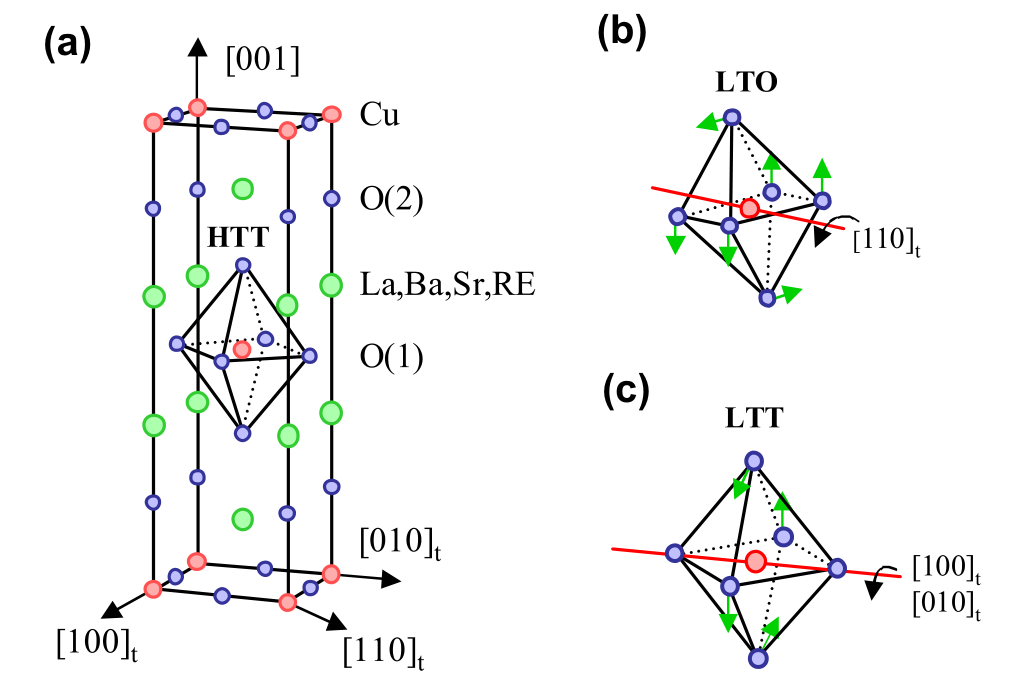
\includegraphics[width=0.8\textwidth]{fig/simulation/crystal_hucker.png}
	\caption[LSCO crystal]{Crystal structure of lanthanum based cuprates. From \cite{Hucker2012}. \todo[inline]{redo figure in orthorhombic coordinates with Q1 and Q2 as tilts}}
	\label{fig:lscocrystal}
\end{figure}

\subsection{Octahedral tilts}
In order to quantify the octahedral tilts, we use the coordinate system sketched in Figure \ref{fig:tilt}. All possible tilts can be described with reference to the LTLO (Pccn) phase. The octahedra are described with two in-plane oxygens (O$_1$, O$_2$) and one apical oxygen $O_3$. Due to symmetry constrains, a rotation of this octahedron will cause a displacements in the $c$-direction of the in-plane oxygen and in the $a$- and $b$-directions of the apical oxygen. Following \cite{Axe1989}, we define $Q_1$ as a rotation around the (010) axis and $Q_2$ as a rotation around the (100) axis in orthorhombic notation. In more intuitive terms, $Q_1$ `tilts' the octahedron along $x$, while $Q_2$ `tilts' along $y$.

\begin{figure}
	\centering
	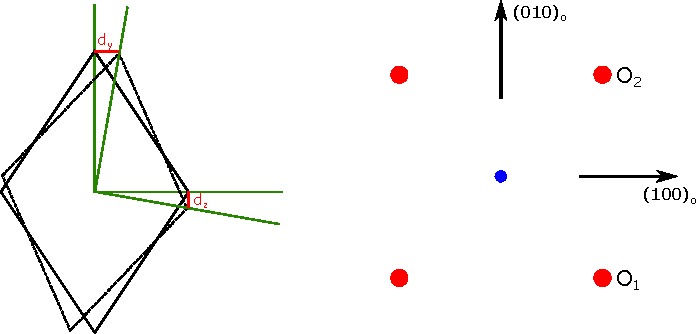
\includegraphics[width=0.8\textwidth]{fig/simulation/tilt.pdf}
	\caption[Geometry of octahedral tilts]{Left: Geometry of octahedral tilts in the with the $c$-axis vertical. Right: Illustration of the two inequivalent in-plane oxygens. The $Q_1$ irreducible representation represents a rotation around the (010) axis while $Q_2$ is a rotation around the (100) axis.\todo[inline]{could use an update}}
	\label{fig:tilt}
\end{figure}

By inspection of Figure \ref{fig:tilt}, a $Q_1$ rotation will displace O$_3$ in the $x$-direction and O$_1$, O$_2$ in the negative $z$-direction. A $Q_2$ rotation will displace O$_3$ in the $y$-direction, O$_1$ in the positive $z$-direction and O$_2$ in the negative $z$-direction. If we want to express $Q_1$ and $Q_2$ as angles, the displacements become:


\begin{align*}
d_x(\text{O}_3) &= | \text{O}_\text{ap} | \sin (Q_1) \frac{c}{a} \\
d_y(\text{O}_3) &= | \text{O}_\text{ap} | \sin (Q_2) \frac{c}{b} \\
d_z(\text{O}_1) &= \frac{1}{4c} \left[ - a \sin (Q_1) + b \sin (Q_2) \right] \\
d_z(\text{O}_2) &= \frac{1}{4c} \left[ - a \sin (Q_1) - b \sin (Q_2) \right] \, ,
\end{align*}

\noindent where $| \text{O}_\text{ap} |$ is the apical oxygen distance, or the $z$-component of O$_3$. Since these equations uniquely define displacements in terms of tilt angles, we can also find tilt angles from structural displacements from either the apical oxygen:

\begin{align*}
Q_1 &= \sin^{-1} \left( \frac{d_x(\text{O}_3)}{| \text{O}_\text{ap} |} \times \frac{a}{c} \right) \\
Q_2 &= \sin^{-1} \left( \frac{d_y(\text{O}_3)}{| \text{O}_\text{ap} |} \times \frac{b}{c} \right) \, ,
\end{align*}

\noindent or the equatorial oxygen:

\begin{align*}
Q_1 &= \sin^{-1}  \left( - \frac{2c}{a} \times (d_z(\text{O}_1) + d_z(\text{O}_2)) \right) \\
Q_2 &= \sin^{-1}  \left( -\frac{4c}{b} \times d_z(\text{O}_2) - \frac{a}{b} \times \sin (Q_1) \right) \, .
\end{align*}

\noindent These equations can then be used to generate desired tilts and extract tilt angles from any given structure.

\subsection{Band Structures}
Band structures are described with respect to the reciprocal lattice. Due to the enlargement of the real-space crystal structure as we move through HTT $\rightarrow$ LTO $\rightarrow$ LTT, the Brillouin Zone (BZ) shrinks by the same amount. Similar to how it is useful to describe our real-space lattice with respect to the LTLO coordinate system, it is useful to describe reciprocal space with respect to a common coordinate system when comparing results. As we can see in Figure \ref{fig:allbz}, the BZ's of HTT, LTO and LTT have vastly different shapes, so it is difficult to superimpose results.

\begin{figure}
	\centering
	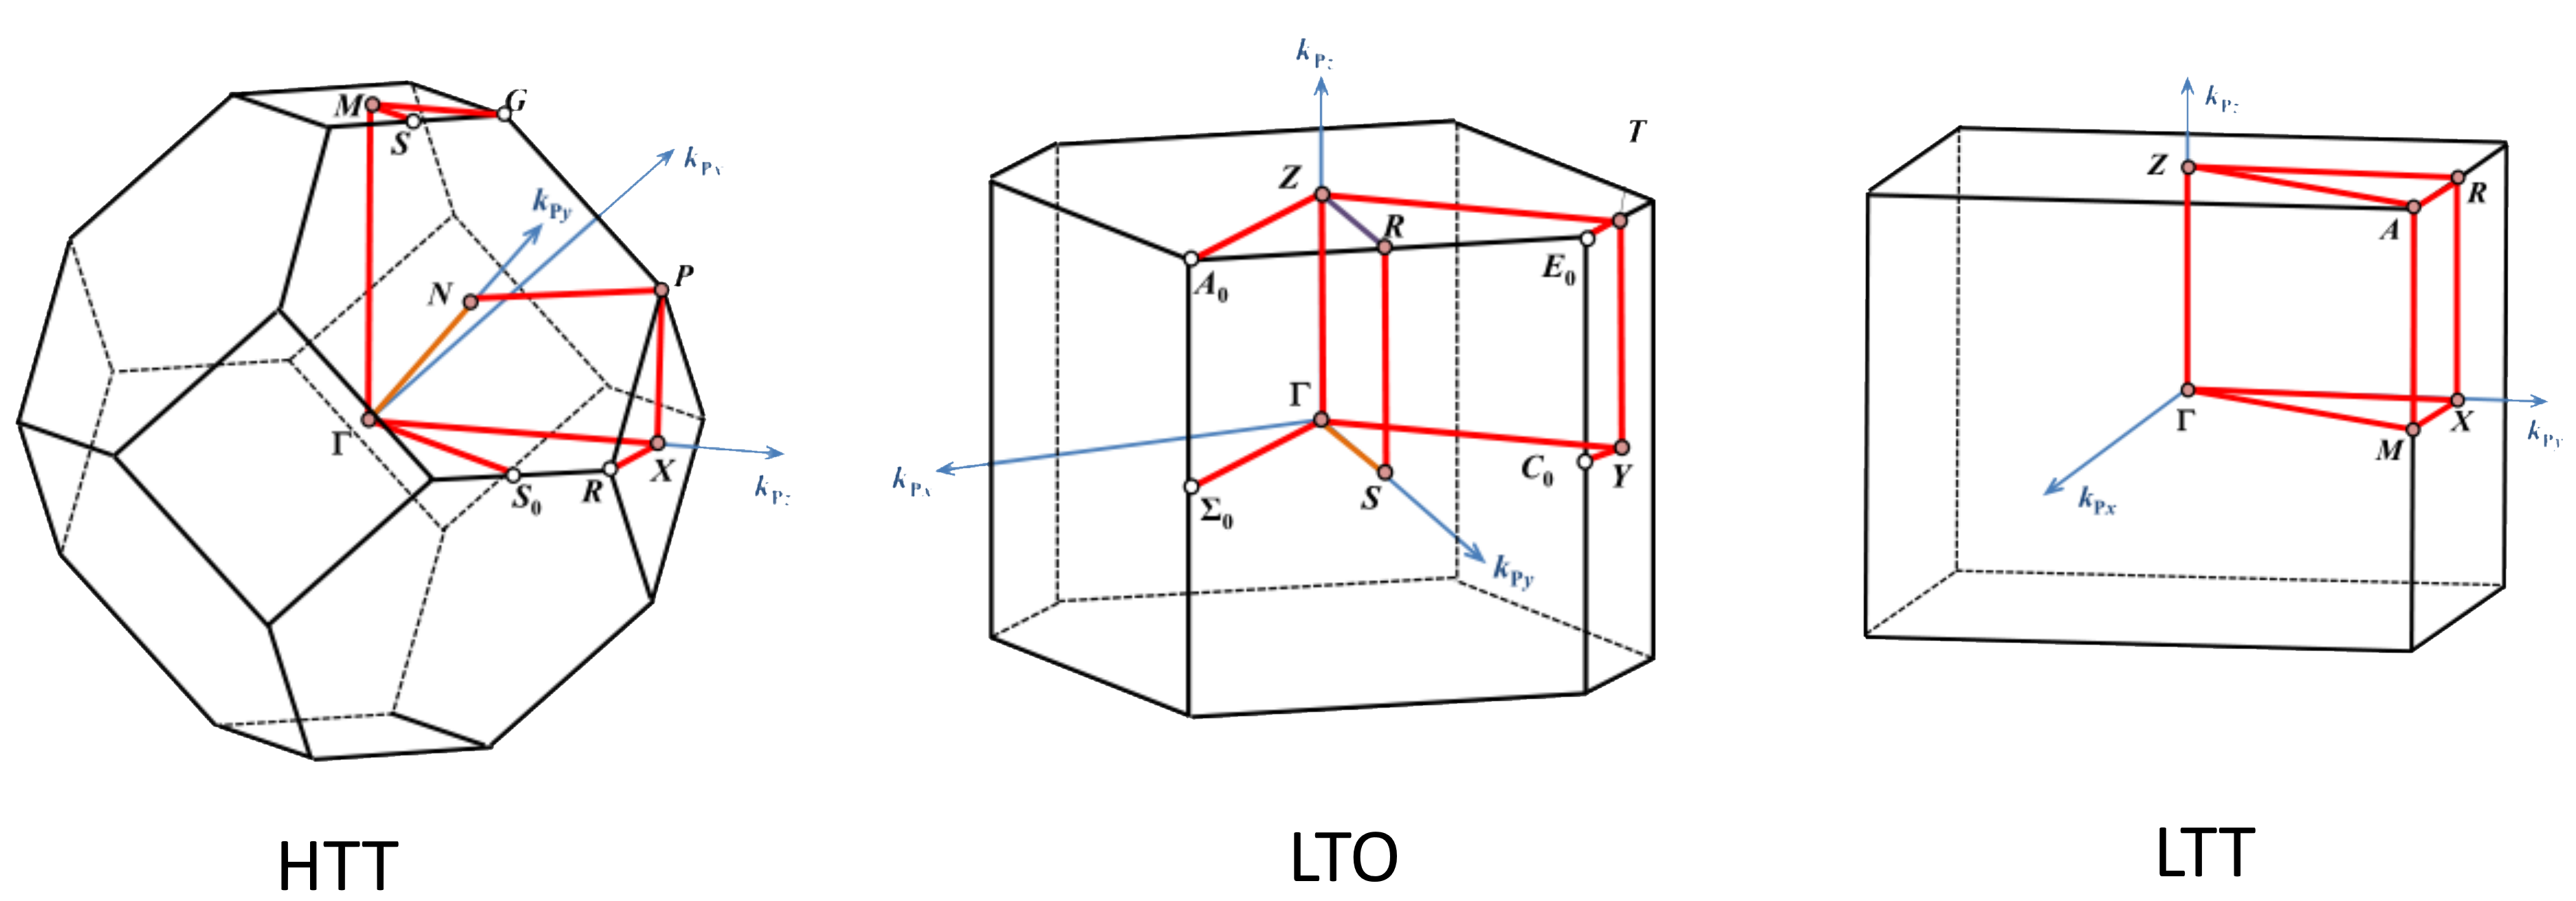
\includegraphics[width=0.8\textwidth]{fig/simulation/BZAll.png}
	\caption[HTT LTO LTT BZs]{BZ of the HTT, LTO and LTT phases. Modified from \cite{Hinuma2017}}
	\label{fig:allbz}
\end{figure}

For this reason, we chose a \emph{primitive} tetragonal BZ to describe the HTT phase and then construct the smaller LTO and LTT BZ's with respect to this construction. The idea is sketched in Figure \ref{fig:band_paths}. This construction also helps emphasize the 2-dimensional nature of the cuprates. In all following simulations, the band labels in Figure \ref{fig:band_paths} will be used, keeping in mind that the nature of high-symmetry points can change depending on the considered structural phase. One example is that the $M$ point, which is the zone boundary of HTT, becomes the zone center of LTO and would thus usually be denoted $\Gamma$.

\begin{figure}
    \centering
    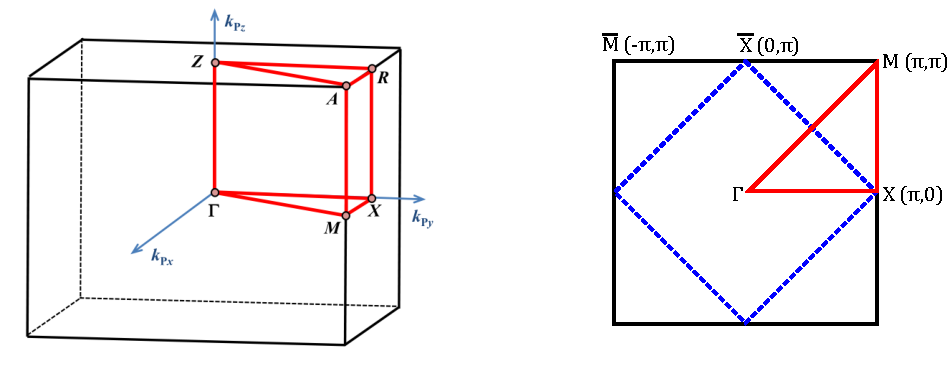
\includegraphics{fig/simulation/band_paths.pdf}
    \caption[Band paths]{\textbf{Left:} BZ of a primitive tetragonal cell with high-symmetry lines. \textbf{Right:} The in-plane BZ with the same labels and the usual $\Gamma$-$X$-$M$-$\Gamma$ path. If the large BZ is the crystallographic HTT phase, then the broken blue lines represent the LTO/LTT/LTLO BZ and we can consider the $\Gamma$-$X$-$\frac{M}{2}$-$\Gamma$ path, since $M$ becomes $\Gamma$ for this (smaller) BZ. In literature the labels are often confused, while $(\pi,\pi)$ and $(\pi,0)$ are universally agreed upon. In any band structure diagrams presented here, the labels in this figure is used.} 
    \label{fig:band_paths}
\end{figure}

While this construction is useful for our intuitive understanding of the different phases, most software expects $k$-vectors with respect to the primitive unit cell. For this reason, we need the transformation matrices from our constructed LTT coordinate system to the primitive HTT and LTO unit cells. This conversion can be done with the following matrices.

\[
\text{PA(HTT)} =  
\begin{pmatrix}
0 & 0 & \frac{1}{2} \\
\frac{1}{2} & \bar{\frac{1}{2}} & 0 \\
\frac{1}{2} & \frac{1}{2} & \bar{\frac{1}{2}}
\end{pmatrix}
\qquad
\text{PA(LTO)} =  
\begin{pmatrix}
\frac{1}{2} & \frac{1}{2} & 0 \\
0 & 0 & 1 \\
\frac{1}{2} & \bar{\frac{1}{2}} & 0
\end{pmatrix}
\]

\noindent these matrices can be used to generate $k$-points starting from the more `intuitive' notation outlined in Figure \ref{fig:band_paths}. For example, the $X$-point ($(\frac{1}{2} \frac{1}{2} 0)$ with respect to LTT) in the HTT phase becomes $(\frac{1}{2} \frac{1}{2} 0) \cdot \text{PA(HTT)} = (\frac{1}{4} \bar{\frac{1}{4}} \frac{1}{4})$.\todo{Double-check this. It works for the band structures, but still not sure why. Relation to real-space transformation matrices?}

\section{VASP Simulation details}


\section{Benchmarking}
When performing DFT calculations in VASP there are a few parameters that have significant impact on the precision of the calculation. Increasing the precision also results in significantly longer computation time, so it is important to find a compromise. 

Figure \ref{fig:sim_bench_afm} shows a benchmark of AFM LCO with respect to the $k$-point mesh and smearing width $\sigma$. Since there are no states at the Fermi level, the smearing width converges rather quickly, and we can safely use a value of $\sigma = \SI{0.1}{\eV}$. The $k$-point density also converges rather quickly, and we achieve a precision of \SI{0.1}{\milli\eV} using a fairly coarse MP-grid of $8\times 8 \times 4$. In AFM LCO we also checked the effect on electronic structure due to the on-site repulsion $U$. The result is shown in Table \ref{tab:ldau}

\begin{figure}
    \centering
    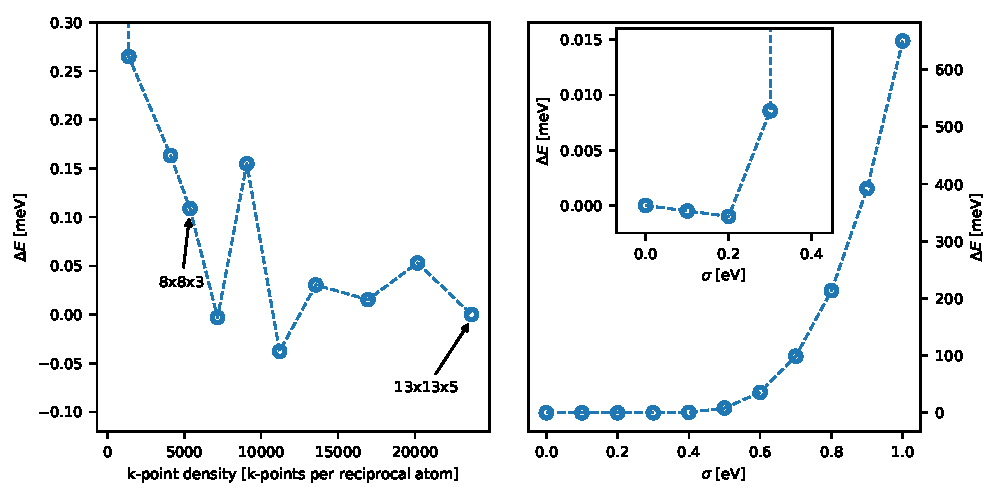
\includegraphics{fig/simulation/convergence_afm.pdf}
    \caption[Simulation Benchmarks: GGA+U]{Simulation Benchmarks: GGA+U with $U=\SI{8}{\eV}$ and $J=\SI{0.8}{\eV}$. \textbf{Left:} Energy as a function of k-point density with $\sigma=\SI{0.1}{\eV}$. $\Delta E$ is total energy (with entropy) with respect to the $13 \times 13 \times 5$ mesh. \textbf{Right:} $\Delta E$ as a function of smearing $\sigma$, where $\sigma=0$ corresponds to the tetrahedron method (\texttt{ISMEAR=-5}).}
    \label{fig:sim_bench_afm}
\end{figure}

\begin{table}[b]
	\centering
	\begin{tabular}{@{}llll@{}}
		\toprule
		U [eV] & J [eV] & Moment [$\mu_\text{B}$] & Optical gap [eV] \\ \midrule
		4.0    & 0.4    & 0.330       & 0.348    \\
		6.0    & 0.6    & 0.481       & 1.016    \\
		8.0    & 0.8    & 0.588       & 1.686    \\
		10.0   & 1.0    & 0.676       & 1.877    \\
		12.0   & 1.2    & 0.755       & 2.042    \\ \bottomrule
	\end{tabular}
	\caption[LDA+U Benchmarking]{LDA+U Benchmarking}
	\label{tab:ldau}
\end{table}

Due to partial occupancies, metallic systems are generally more sensitive to $k$-point density and smearing width/method. For this reason, we performed a more comprehensive set of benchmarks as shown in Figure \ref{fig:sim_bench_para}. While the numerical fluctuations are still within a few meV, the precision on total energy is decreased by a few orders of magnitude.

\begin{figure}
    \centering
    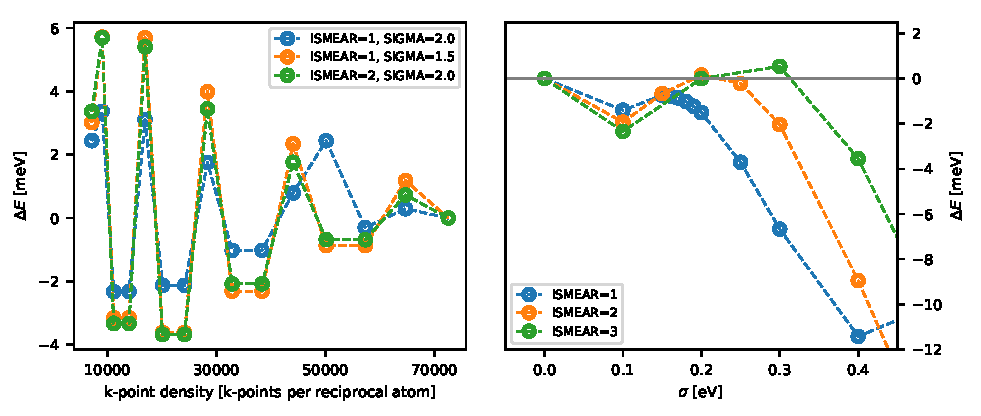
\includegraphics{fig/simulation/convergence_metal.pdf}
    \caption[Simulation Benchmarks: Paramagnet/Metal]{Simulation Benchmarks: Paramagnet/Metal. Note the significant variation in energy compared to the insulating case, even with much higher k-point density. \textbf{Left:} Energy as a function of k-point density for three combinations values of $\sigma$ and smearing type. $\Delta E$ is total energy (with entropy) with respect to the $18 \times 18 \times 8$ mesh. \textbf{Right:} $\Delta E$ as a function of $\sigma$ with the Methfessel-Paxton method (orders 1, 2, 3) while using a $16 \times 16 \times 8$ k-point mesh (57344 k-points per reciprocal atom). $\sigma=0$ corresponds to the tetrahedron method (\texttt{ISMEAR=-5}). Below $\sigma = \SI{0.4}{\eV}$ the entropy term is \SI{0.5}{\milli\eV} per atom or lower, so forces should be well-behaved.}
    \label{fig:sim_bench_para}
\end{figure}

%\begin{table}[b]
%	\centering
%	\begin{tabular}{@{}lllll@{}}
%		\toprule
%		& HTT & HTT (metal)  & LTO    & LTT    \\ \midrule
%		a [\AA]         & 5.32 & 5.31 & 5.34   & 5.37   \\
%		c [\AA]         & 12.99 & 13.05 & 13.01  & 12.93  \\
%		O3(z)      & 0.184 & 0.185 & 0.185  & 0.184  \\
%		La(x)      & 0     & 0 & 0      & -0.009 \\
%		La(y)      & 0     & 0 & -0.012 & -0.009 \\
%		La(z)      & 0.362 & 0.362 & 0.361  & 0.361  \\
%		$\eta$ ($\times 100$) & 0  & 0 &  1.465  & 0      \\
%		Q1 (degrees)        & 0 & 0 &  0      & 4.6125 \\
%		Q2 (degrees)        & 0 & 0 &  5.786  & 4.6125 \\ 
%		degrees of freedom & 2 & 2 & 5 & 5 \\ \bottomrule
%	\end{tabular}
%	\caption[HTT, LTO, LTT: Structural parameters]{HTT, LTO, LTT: Structural parameters, defined with a minimal set of parameters based on results from simulations. Q1/Q2 are taken as the average angle from equatorial and apical tilt. The fractional positions of O1, O2 and O3 are completely described using Q1, Q2 and O3(z), Cu is allways at (0,0,0) and $\eta = \frac{b-a}{b+a}$ uniquely defines any difference between $a$ and $b$. In the generation of structures, the Pccn (LTLO) space group is used. Degrees of freedom refers to the atomic positions only. The description of our system in terms of Q1/Q2 thus removes one degree of freedom by coupling the apical and equatorial oxygen.}
%	\label{tab:struct_par}
%\end{table}

\section{Electronic Structure}
While we are generally interested in lattice dynamics, a DFT calculation is leveraging the electronic structure in any simulation. It is thus worthwhile to check if the electronic structure, at least approximately, represents reality. In the cuprates, it is well known that DFT is unable to explain the peculiarities in the superconducting phase. However, we can get fairly close in the limit of zero doping (AFM Mott Insulator) and overdoping (fermi liquid). Figure \ref{fig:edos_htt} compares the electronic density of states of the Mott Insulator and fermi liquid for two different functionals. We clearly see how the DFT+U opens a gap by pushing states below the Fermi level.

\begin{figure}
    \centering
    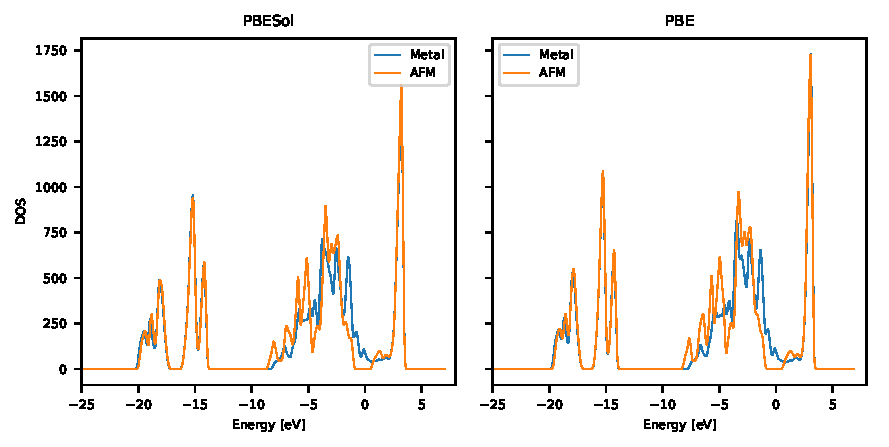
\includegraphics{fig/simulation/htt_dos.pdf}
    \caption[Electronic DOS: Metal and AFM]{Electronic density of states for HTT phase with two different functionals in a metallic (paramagnetic) and AFM (GGA+U) states. The two functionals appear to describe the system identically. The AFM state is shifted by \SI{-1}{\eV} for comparative purposes (which is why the Fermi level is in the middle of the gap).}
    \label{fig:edos_htt}
\end{figure}

To further illustrate this point, Figure \ref{fig:bs_afm2} and \ref{fig:bs_metal} shows the band structure coloured by atomic projections in the AFM and metallic state, respectively. We now notice that DFT+U is pushing the Cu states down, as expected from the on-site respulsion.

\begin{figure}
    \centering
    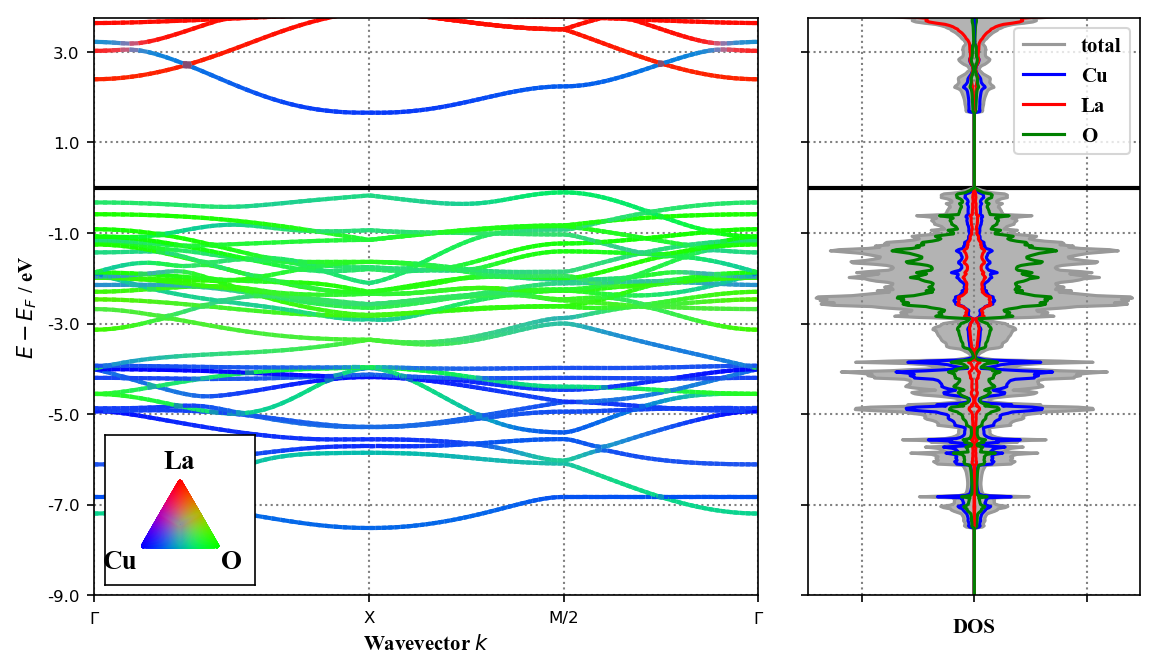
\includegraphics[width=\textwidth]{fig/simulation/bs_afm2.png}
    \caption[GGA+U: AFM Electronic Band Structure]{GGA+U: AFM Electronic Band Structure of the Bmab LTO structure along the $\Gamma$-$X$-$\frac{M}{2}$-$\Gamma$ path (LTO high symmetry lines). The upper and lower Hubbard bands are clearly visible and are separated by \SI{8}{\eV} as expected.}
    \label{fig:bs_afm2}
\end{figure}

%\begin{figure}
%    \centering
%    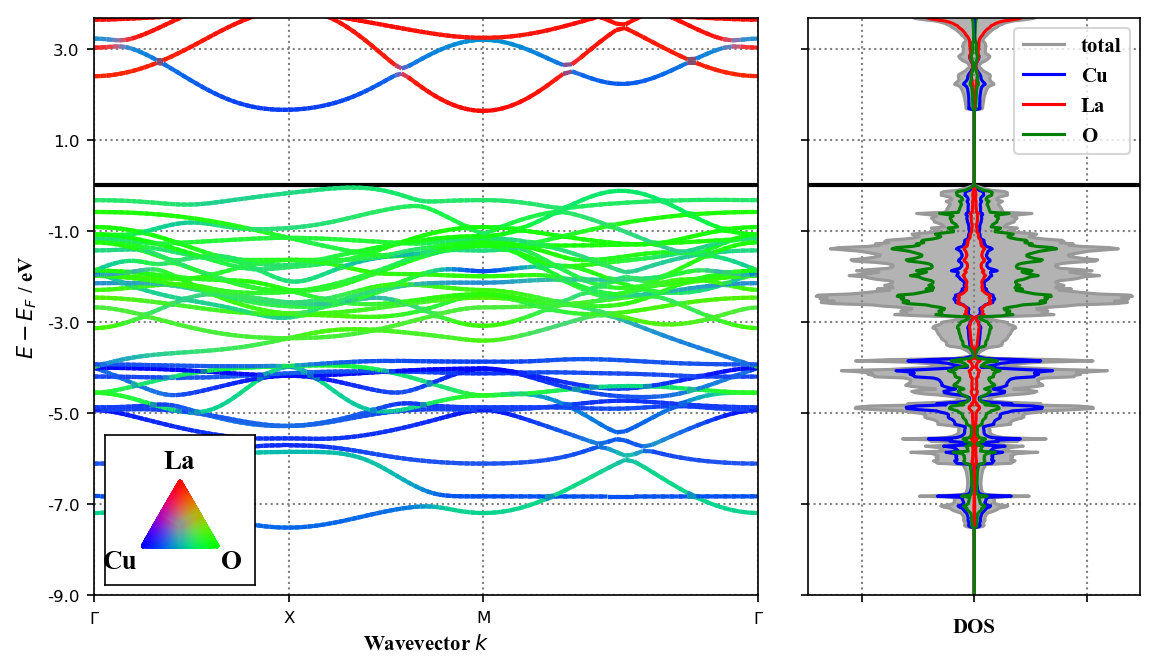
\includegraphics[width=\textwidth]{fig/simulation/bs_afm1.png}
%    \caption[GGA+U: AFM Electronic Band Structure]{GGA+U: AFM Electronic Band Structure of the Bmab LTO structure along the $\Gamma$-$X$-$M$-$\Gamma$ path (HTT high symmetry lines). The upper and lower Hubbard bands are clearly visible and are separated by \SI{8}{\eV} as expected.}
%    \label{fig:bs_afm1}
%\end{figure}

\begin{figure}
    \centering
    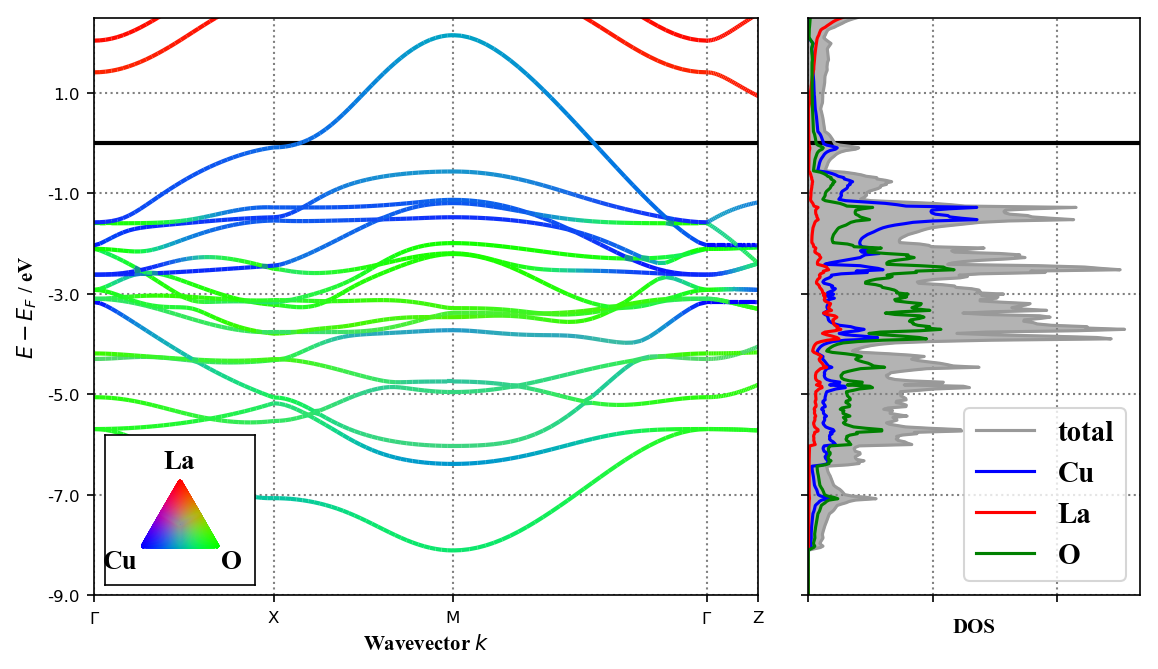
\includegraphics[width=\textwidth]{fig/simulation/bs_metal.png}
    \caption[GGA: Metallic Electronic Band Structure]{Metallic Electronic Band Structure of the I4/mmm HTT structure. Path is through the high-symmetry points as defined in Figure \ref{fig:band_paths} with respect to the conventional unit cell. The $\Gamma$-$Z$ path is shown to illustrate the 2-dimensional nature of the electronic structure (The dispersion is relatively flat).}
    \label{fig:bs_metal}
\end{figure}

\section{Geometry optimization}
Optimizing geometry in VASP can be performed with 3 different algorithms controlled by the \texttt{IBRION} tag\todo{references}:

\begin{enumerate}
	\item RM-DIIS
	\item Conjugate Gradient (CG)
	\item Damped molecular dynamics
\end{enumerate}

\noindent All algorithms requires to set the \texttt{POTIM} tag which controls the step-size. Usually the default value of 0.5 is reasonable. Damped molecular dynamics requires a damping factor in addition, set by the \texttt{SMASS} tag. For this reason RM-DIIS and CG require less user intervention and are good first choices. While RM-DIIS is usually a good choice for systems close to equilibrium, it struggles with rigid unit modes such as octahedral tilts in perovskites. Since these tilts are at the centre of our investigation, we use CG in most cases.

The optimization routine is constrained by the point group symmetry as determined by VASP. The \texttt{ISIF} tag controls how the positions, cell shape and cell volume is updated during the optimization. It might seem obvious to simply optimize everything, but for complex problems convergence can be problematic. In addition, changing the cell volume changes the basis set\footnote{The basis set is defined by the number of plane waves up to a certain frequency that fits in the unit cell. If the unit cell dimensions change, so do the set of plane waves.}. VASP explicitly avoids changing the basis set during volume optimizations, resulting in the so-called \emph{Pulay stress} due to incompleteness of the basis set. In practice, there are two primary strategies for getting accurate geometry optimizations. The first is a step-wise optimization of parameters in the scheme

\begin{quote}
	Coordinates $\rightarrow$ Coordinates/Shape $\rightarrow$ Coordinates/Shape/Volume
\end{quote}

\noindent The second is perform successive coordinate/shape optimizations at a set of volumes and fit the resulting volume-energy curve to an equation of state. While this method is more computationally expensive, it provides us with additional information about volume-dependent behaviour such as the bulk modulus. In practice we use the exponential equation of state formulated by \citeauthor{Vinet1987}\cite{Vinet1987}:

\begin{equation*}
\tiny
E(V) = E_0 + \frac{2B_0V_0}{\left(B_0^\prime-1\right)^2}\left\lbrace 2 -\left[ 5 + 3\left( \frac{V}{V_0}\right)^\frac{1}{3} (B_0^\prime -1)  -3B_0^\prime \right] \right. \left. \exp \left[ -\frac{3}{2} \left( B_0^\prime-1\right)\left[\left( \frac{V}{V_0}\right)^\frac{1}{3} -1\right]\right]\right\rbrace
\end{equation*}

\noindent where $V_0$ is the equilibrium volume, $B_0$ is the bulk modulus and 

\begin{equation*}
B_0^\prime = \left( \frac{\partial B_0}{\partial P}\right)_T
\end{equation*}

\subsection{Geometry of AFM LCO}
We performed equation-of-state fits to AFM LCO in all three structural phases. Figure \ref{fig:eos_afm_all} shows the Energy-Volume fits, Figure \ref{fig:eos_ratios_afm} shows the volume dependence of the cell ratios and Figure \ref{fig:angles_afm} shows how the angles in the LTO and LTT phases change as a function of volume. Contrary to experiment, the LTO phase is energetically unfavourable and the favoured phase is LTT. Figure \ref{fig:angles_afm} reveals that the $Q_1$ and $Q_2$ are not exactly rigid, consistent with experiment. Intuitively, it is `easier' to move the apical oxygen due to the rocksalt-layer being less dense.\todo{Maybe overkill with 3 graphs for a few simple conclusions? 6 if we count the metallic counterparts}


\begin{figure}
    \centering
    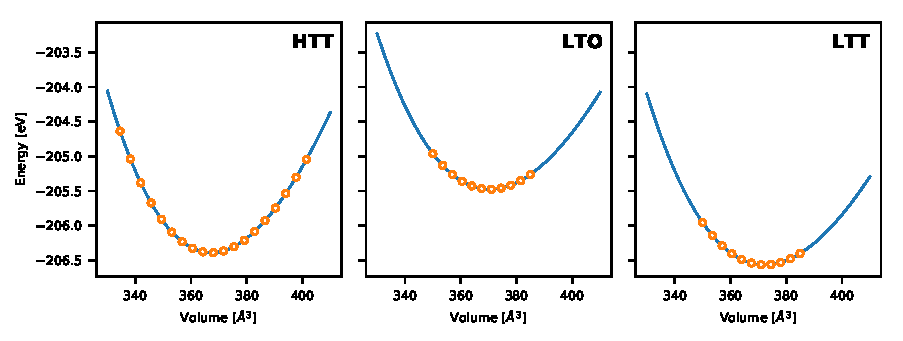
\includegraphics[width=\textwidth]{fig/simulation/eos_all.pdf}
    \caption[AFM: Equation-of-state fits]{Equation-of-state fits (AFM). Optimal volume of simulated structures are found by performing optimization of fractional coordinates and cell shape at a series of fixed volumes. The resulting Energy/Volume curve is then fit to a Vinet exponential equation of state \cite{Vinet1987}. This is done for the HTT, LTO and LTT phases with the PBESol functional.}
    \label{fig:eos_afm_all}
\end{figure}

\begin{figure}
    \centering
    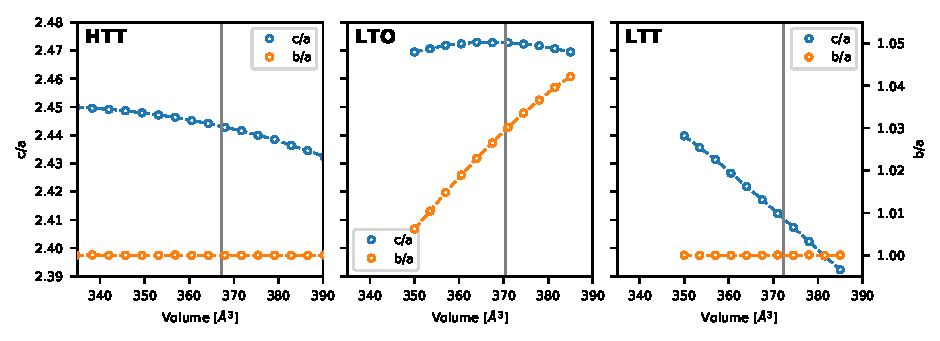
\includegraphics[width=\textwidth]{fig/simulation/ratio_all.pdf}
    \caption[AFM: Cell ratios during EOS fits]{Cell Ratios (AFM). During the equation-of-states fits from Figure \ref{fig:eos_afm_all}, the cell shape is modified, changing the $b/a$ ratio (orthorhombicity) and $c/a$ ratio (larger values correspond to a cell that is elongated along $c$). Due to symmetry $b/a = 1$ for the HTT and LTT phases. Vertical line is the optimal volume from the fit.}
    \label{fig:eos_ratios_afm}
\end{figure}

\begin{figure}
    \centering
    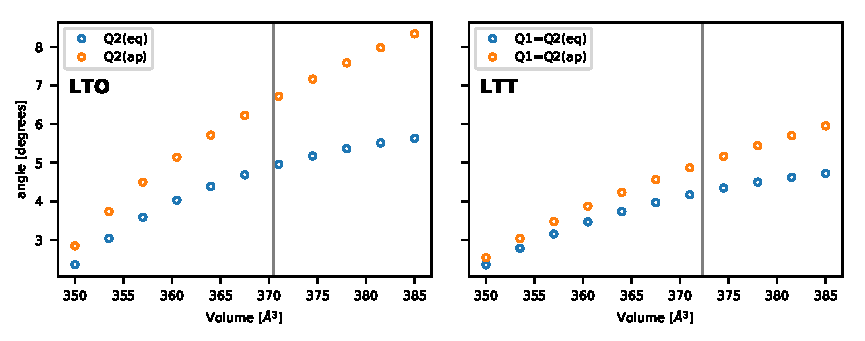
\includegraphics[width=\textwidth]{fig/simulation/angles_lto_ltt.pdf}
    \caption[AFM: LTO/LTT angles during EOS fits]{LTO/LTT Angles (AFM) During equation-of-state fits, we record the tilt angles for the LTO and LTT phase. Here, they are plotted as a function of Volume. Note that for LTO $Q_1=0$ and for LTT $Q_1=Q_2$. However, the rotation angle is measured differently from the equatorial (eq) and apical (ap) oxygen. The difference in values can be thought of as `non-rigidity' of the rotation.}
    \label{fig:angles_afm}
\end{figure}

\subsection{Geometry of metallic LCO}
The same geometry optimization was performed in the metallic state of LCO. Equation-of-state fits are shown in Figure \ref{fig:eos_metal_all}, cell ratios are shown in Figure \ref{fig:eos_ratios_metal} and the LTO/LTT angles are shown in Figure \ref{fig:angles_metal}. Qualitatively, we notice very similar behaviour to AFM LCO, but for these calculations LTT and LTO are the preferred phases with very similar total energies.


\begin{figure}
    \centering
    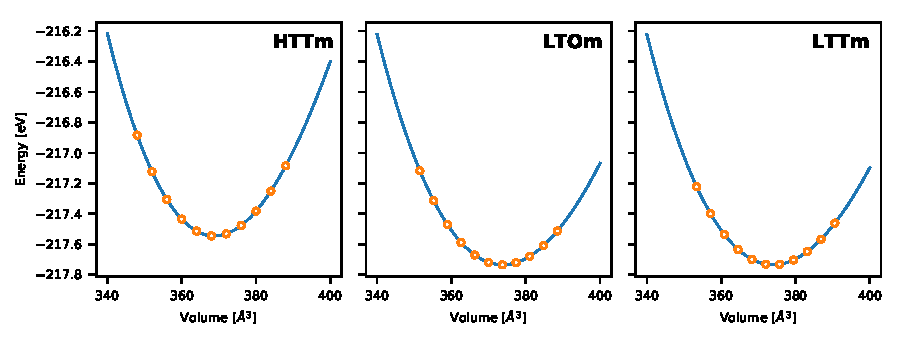
\includegraphics[width=\textwidth]{fig/simulation/eos_metal_all.pdf}
    \caption[Metal: Equation-of-state fits]{Equation-of-state fits (Metal). Optimal volume of simulated metallic structures are found by performing optimization of fractional coordinates and cell shape at a series of fixed volumes. The resulting Energy/Volume curve is then fit to a Vinet exponential equation of state \cite{Vinet1987}. This is done for the HTT, LTO and LTT phases with the PBESol functional.}
    \label{fig:eos_metal_all}
\end{figure}

\begin{figure}
    \centering
    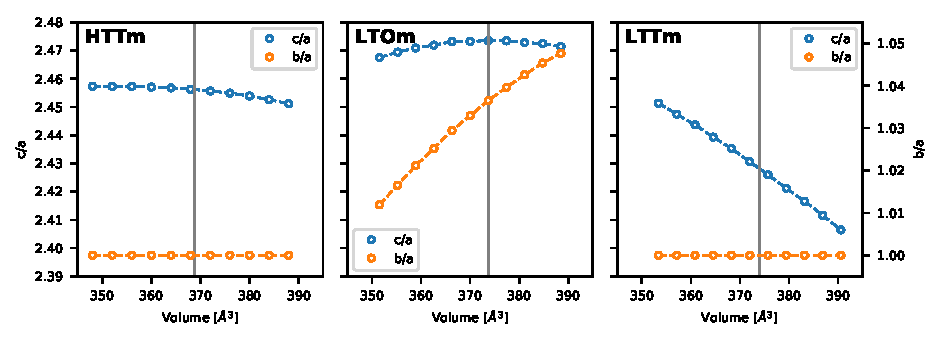
\includegraphics[width=\textwidth]{fig/simulation/ratio_metal_all.pdf}
    \caption[Metal: Cell ratios during EOS fits]{Cell ratios (Metal). During the equation-of-states fits from Figure \ref{fig:eos_metal_all}, the cell shape is modified, changing the $b/a$ ratio (orthorhombicity) and $c/a$ ratio (larger values correspond to a cell that is elongated along $c$). Due to symmeetry $b/a = 1$ for the HTT and LTT phases. Vertical line is the optimal volume from the fit.}
    \label{fig:eos_ratios_metal}
\end{figure}

\begin{figure}
	\centering
	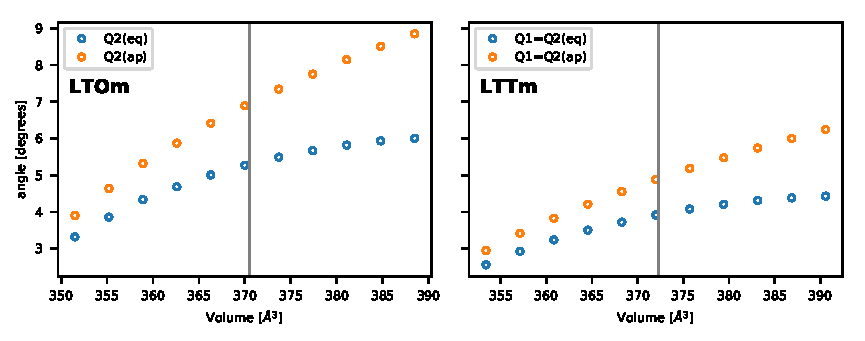
\includegraphics[width=\textwidth]{fig/simulation/angles_metal_lto_ltt.pdf}
	\caption[Metal: LTO/LTT angles during EOS fits]{LTO/LTT angles (Metal). During equation-of-state fits, we record the tilt angles for the LTO and LTT phase. Here, they are plotted as a function of Volume. Note that for LTO $Q_1=0$ and for LTT $Q_1=Q_2$. However, the rotation angle is measured differently from the equatorial (eq) and apical (ap) oxygen. The difference in values can be thought of as `non-rigidity' of the rotation.}
	\label{fig:angles_metal}
\end{figure}


\subsection{Summary of geometry optimization}
A summary of all the geometry optimizations are shown in Table \ref{tab:sim_struct}. Additional data from simulations with a different functional have been added to this table. We notice that the PBE functional finds a volume closer to experimental value, but phonon calculations show a more consistent behaviour of the PBESol functional.


\begin{table}
    \centering
    \begin{tabular}{lllllllllll}
\toprule
structure &  phase & encut &      XC &       E0 &       V0 &    c/a &    $\eta$ &     $Q_1$ &     $Q_2$ \\
\midrule
      HTT &    afm &   520 &     PBE & -194.352 &  383.410 &  2.431 &  0.000 &  0.000 &  0.000 \\
      HTT &    afm &   800 &     PBE & -194.494 &  383.297 &  2.430 &  0.000 &  0.000 &  0.000 \\
      HTT &    afm &   800 &  PBESol & -206.390 &  367.310 &  2.443 &  0.000 &  0.000 &  0.000 \\
      LTO &    afm &   800 &  PBESol & -205.476 &  370.500 &  2.437 &  1.465 &  0.000 &  5.786 \\
      LTT &    afm &   800 &  PBESol & -206.565 &  372.282 &  2.410 &  0.000 &  4.612 &  4.612 \\
      HTT &  metal &   800 &  PBESol & -217.546 &  368.774 &  2.456 &  0.000 &  0.000 &  0.000 \\
      LTO &  metal &   800 &  PBESol & -217.735 &  373.793 &  2.430 &  1.795 &  0.000 &  6.421 \\
      LTT &  metal &   800 &  PBESol & -217.735 &  373.948 &  2.428 &  0.000 &  4.528 &  4.528 \\
\bottomrule
\end{tabular}

    \caption[Simulation Structure Results]{Resulting structure due to EOS fits to various structural phases and functionals. The two values given for $Q_1$/$Q_2$ are angles calculated from equatorial and apical oxygens, respectively. Interestingly, in terms of energy LTT $<$ HTT $<$ LTO, while the phonons are `more unstable' for HTT than LTO (See Figures \ref{fig:htt_bands}, \ref{fig:lto_bands}, \ref{fig:ltt_bands}). For the metallic cases, we note the optimal geometry is similar to the magnetic case. While the energy is lower, it is not meaningful to compare total energies between GGA+U and GGA.}
    \label{tab:sim_struct}
\end{table}

\section{Phonon bands}
Phonon calculations were performed on both metallic and AFM LCO in the HTT, LTO and LTT structrual phases. While benchmarking with regards to $k$-points and smearing width $\sigma$ is reasonable, we check the effect of functional choice and energy cut-off \texttt{ENCUT} on phonon bands. In Figure \ref{fig:pbe_bands}, we show the phonon band structure in the AFM phase with \texttt{ENCUT=520} and \texttt{ENCUT=800}. While the effect of increasing the plane wave cut-off is small, we see immediately that it fixes some unstable modes at $\Gamma$. While we do expect instabilities at the $M$ point in the HTT phase, the results could be improved.

\begin{figure}
	\centering
	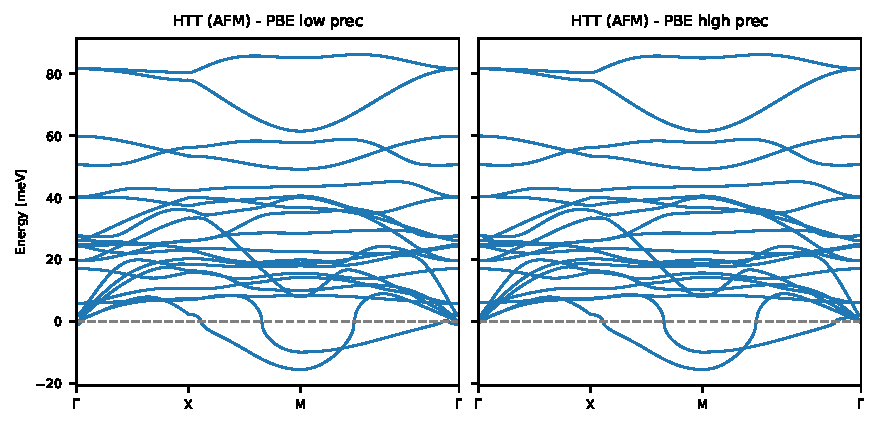
\includegraphics[width=\textwidth]{fig/simulation/htt_pbe_bands.pdf}
	\caption[PBE Bands: Comparison wrt ENCUT]{Phonon band structure of LCO in the HTT phase using the PBE functional with a \SI{520}{\eV} (low prec]) and \SI{800}{\eV} (high prec) plane wave cut-off. Both simulations are performed using a magnetic electronic structure within the DFT+U formalism.}  
	\label{fig:pbe_bands}
\end{figure}

For this reason, we keep the \SI{800}{\eV} cut-off and perform the same phonon calculation using the PBESol \cite{Csonka2009} functional. This functional has been successful for phonon calculations in other perovskite systems \cite{DaSilva2015}, so it is a likely candidate for improvement. Figure \ref{fig:htt_bands} shows phonon band structures in the HTT phase using both AFM and metallic electronic structures. We immediately notice improvements on two fronts. First, the low-energy modes are `more stable' and the unstable modes are localized around $M$ where we expect instabilities. Second, the high-energy bond-strething mode ($\Gamma$-$X$) has increased in energy and is much closer to experimental values. In addition, we reproduce the softening of this mode at the zone boundary due to doping.

\begin{figure}
	\centering
	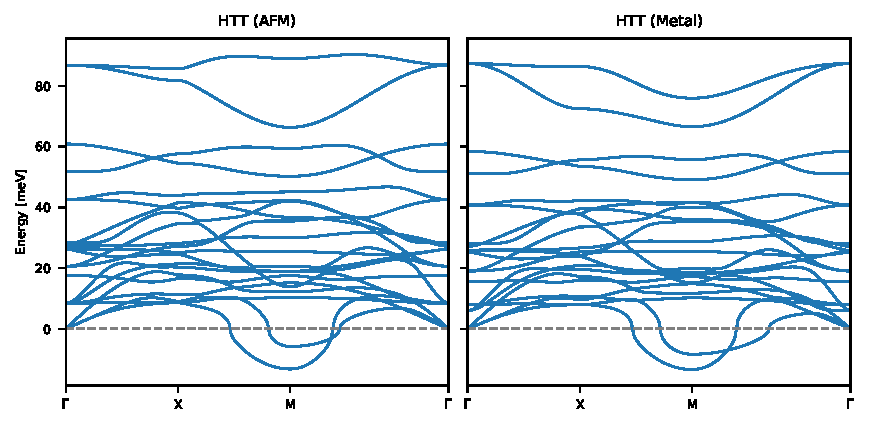
\includegraphics[width=\textwidth]{fig/simulation/htt_bands.pdf}
	\caption[HTT Bands]{Phonon band structure of LCO in the HTT phase using the PBESol functional and an 800 eV plane-wave cut-off. The high-symmetry lines are with respect to the primitive tetragonal BZ (See Figure \ref{fig:band_paths})}
	\label{fig:htt_bands}
\end{figure}

While there, in principle, are a huge number of functionals one could try, phonon calculations are quite expensive and the PBESol results are reasonable in the context of lattice dynamics. We thus stick to the PBESol functional in simulations moving forward.

To check the stability of structural phases in LCO, we perform phonon calculation in the LTO and LTT phases, shown in Figure \ref{fig:lto_bands} and \ref{fig:ltt_bands}. Qualitatively, we see similar features to HTT (apart from the obvious increase of bands). The most significant result is that the LTO and LTT phases clearly stabilizes at the $M$-point, suggesting that our simulations reproduce the observed structural phase transitions. The stability of LTT is particularly interesting in this case, since this phase is believed to suppress superconductivity. In particular when combined with the fact that LTO and LTT are very close in energy when looking at the metallic simulations.

\begin{figure}
	\centering
	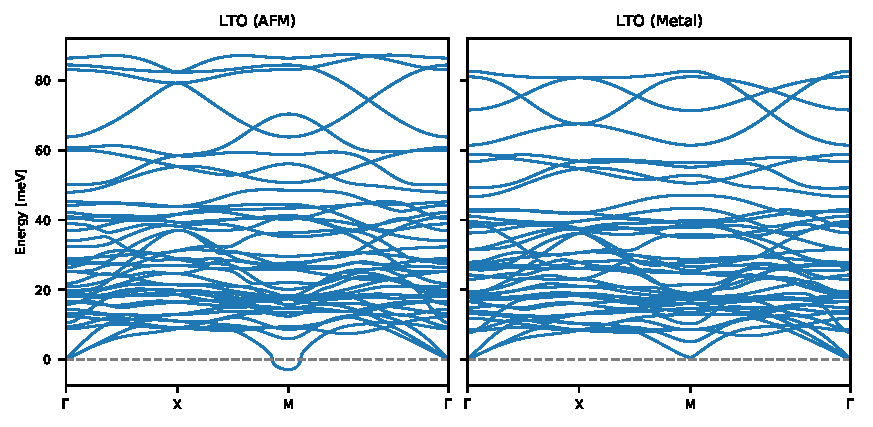
\includegraphics[width=\textwidth]{fig/simulation/lto_bands.pdf}
	\caption[LTO Bands]{Phonon band structure of LCO in the LTO phase using the PBESol functional and an 800 eV plane-wave cut-off. The high-symmetry lines are with respect to the primitive tetragonal BZ (See Figure \ref{fig:band_paths})}
	\label{fig:lto_bands}
\end{figure}

\begin{figure}
	\centering
	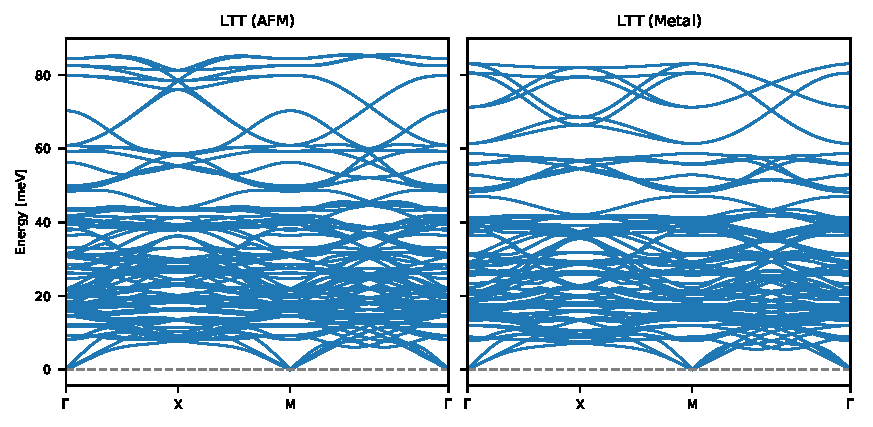
\includegraphics[width=\textwidth]{fig/simulation/ltt_bands.pdf}
	\caption[LTT Bands]{Phonon band structure of LCO in the LTT phase using the PBESol functional and an 800 eV plane-wave cut-off. The high-symmetry lines are with respect to the primitive tetragonal BZ (See Figure \ref{fig:band_paths})}
	\label{fig:ltt_bands}
\end{figure}

\section{Phonon DOS}
The phonon density-of-states is formally defined as

\[ g(\omega) = \frac{1}{N} \sum_\lambda \delta(\omega - \omega _\lambda) \]

\noindent where $\omega$ is the phonon frequency, $N$ is the number of unit cells and $\omega _\lambda$ is the energy of a phonon $\lambda=(\nu,\bm{q})$ parametrized by a band index $\nu$ and a wave vector $\bm{q}$. In practice, $g(\omega)$ is found by integrating the phonon branches in the FBZ on a mesh of $N$ equally spaced points. The $\delta$-function is handled by either replacing it with a Gaussian of finite width $\sigma$ or by performing an integration using the tetrahedron method \cite{Blochl1994} (or both)\todo{sill not sure how it is ACTUALLY done in phonopy}. The partial density of states an atom $j$ can similarly be defined as:

\[ g^j (\omega) = \sum_{\bm{\hat{n}}=\{x,y,z\}} \frac{1}{N} \sum_\lambda \sigma(\omega - \omega_\lambda) \left| \bm{\hat{n}} \cdot \bm{e}^j_\lambda \right| ^2 \]

\noindent where $\bm{\hat{n}}$ is the unit projection vector direction and $\bm{e}^j_\lambda$ is the phonon eigenvector of atom $j$ at $\lambda=(\nu,\bm{q})$. The neutron-weighted partial density of states of atom $j$ is then simply $b_j g^j(\omega)$, where $b_j$ is the total scattering cross-section of atom $j$.

\begin{figure}
	\centering
	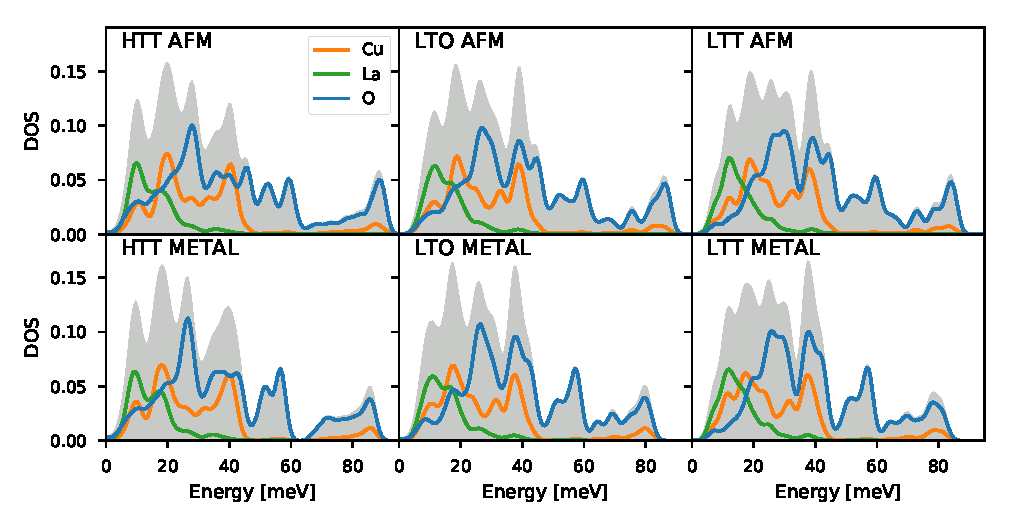
\includegraphics[width=\textwidth]{fig/simulation/phonopy_pdos.pdf}
	\caption[Neutron DOS (frozen-phonons)]{Neutron-weighted phonon density of states in the various structural and electronic phases of LCO. Both the partial and total density of states is shown in the plot.}
	\label{fig:dos_all}
\end{figure}

Figure \ref{fig:dos_all} shows the neutron weighted partial and total density of states due to the 6 different phonon calculations we performed. The density of states was evaluated on a $48 \times 48 \times 48$ grid, integrated using the tetrahedron method and an applied Gaussian smearing of $\sigma=\SI{1}{\milli\eV}$ (\SI{2.35}{\milli\eV} FWHM). To get comparable values of $g(\omega)$, the plots are normalized to the BZ volume ($4V^\text{BZ}_\text{HTT} = 2 V^\text{BZ}_\text{LTO} = V^\text{BZ}_\text{LTT}$).

\section{Validation of simulations}
Since LSCO is such an extensively studied system, there is data available in the literature to compare our band structures. By inspection of the band structure plots in the previous section, it seems like a difficult task to actually separate the bands in a neutron scattering experiment. Luckily, there are a few LO modes that can be distinguished. Figure \ref{fig:htt_phonons_lit} compares our HTT band phonons band structures along $\Gamma$-$X$ with experimental data from a range of LSCO samples. The highlighted modes is the Cu-O half-breathing mode ($\approx \SI{80}{\milli\eV}$) and the apical oxygen stretching mode ($\approx \SI{60}{\milli\eV}$).

\begin{figure}
	\centering
	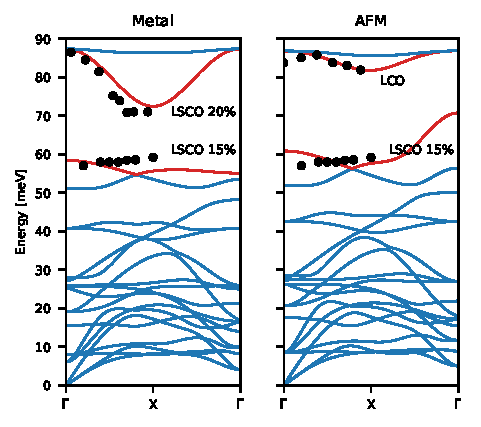
\includegraphics[width=0.7\textwidth]{fig/simulation/htt_phonons_lit.pdf}
	\caption[phonon bands: comparison with literature]{Comparison of phonon band structures in the HTT structural phase along the $\Gamma$-X path with data from literature. Modes associated with data are highlighted in red.\todo[inline]{references to data + giustino}}
	\label{fig:htt_phonons_lit}
\end{figure}

Similarly, we can compare the phonon density of states to time of flight powder measurements. Figure \ref{fig:dos_comparison} shows the LTT simulations along with data from IN4c on the parent compound LCO.

\begin{figure}
	\centering
	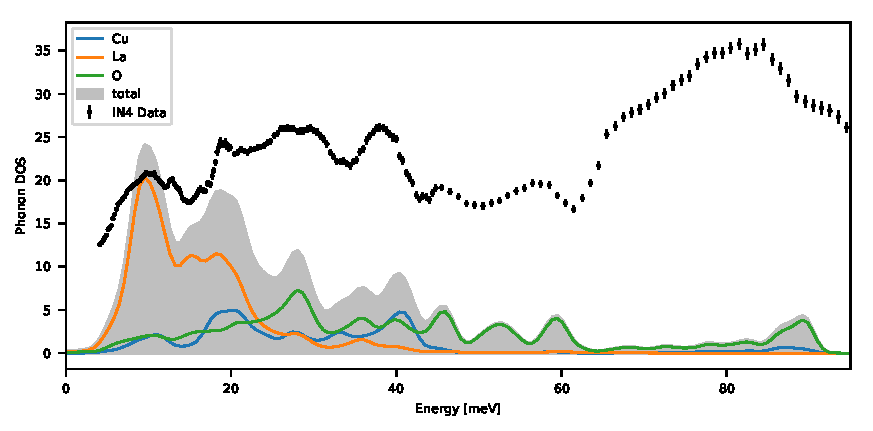
\includegraphics[width=\textwidth]{fig/simulation/dos_comparison.pdf}
	\caption[phonon dos: comparison with IN4]{Comparison of the neutron-weighted phonon density of states as calculated for the LTT (AFM) phase with neutron data from IN4. Simulation data has been smeared by a width of $\sigma=\SI{1}{\milli\eV}$.\todo[inline]{maybe a scaling that depends on energy?}}
	\label{fig:dos_comparison}
\end{figure}

\section{Neutron-weighted phonon bands}

\begin{figure}
	\centering
	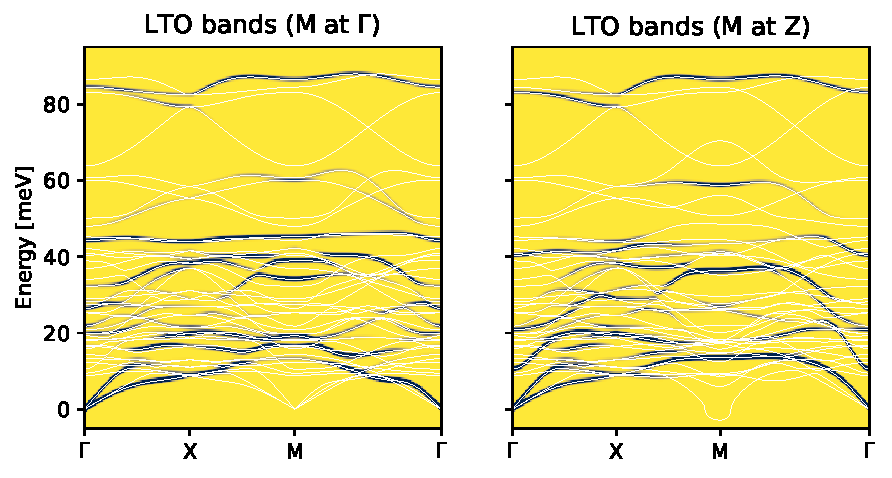
\includegraphics[width=\textwidth]{fig/simulation/lto_neutron_bands.pdf}
	\caption[LTO band structure with neutron intensities]{LTO band structure with neutron intensities. $l=0$ so no intensity at $Z$. The wo paths are with respect to Figure \ref{fig:band_paths}. but in the two inequivalent directions due to orthorhombic strain. A real neutron scattering image would correspond to the superposition of these two band structures due to twinning.}
	\label{fig:lco_lto_netron_bands}
\end{figure}

\begin{figure}
	\centering
	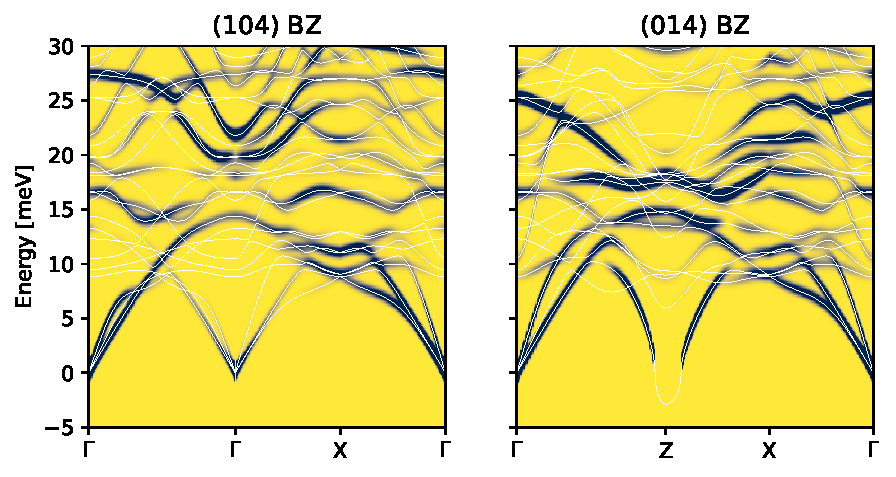
\includegraphics[width=\textwidth]{fig/simulation/lco_soft_modes.pdf}
	\caption[LCO, LTO: soft mode simulation]{Neutron-weighted phonon bands of the LTO taken in the (104) and (014) BZ along the $M$-$\Gamma$-$X$-$M$ (left to right) path with respect to the coordinate system defined in Figure \ref{fig:band_paths}. Due to the larger BZ of the LTO primitive cell, the high symmetry points changes their labels as shown on the horizontal axis of the figure. This illustrates the fact that neutron scattering measurements at (104)/(014) will be measuring at the primitive $\Gamma$- and $Z$-point, respectively. Note that an $l$-component is required to get any neutron weight at $Z$.}
	\label{fig:lco_soft_sim}
\end{figure}

\begin{figure}
	\centering
	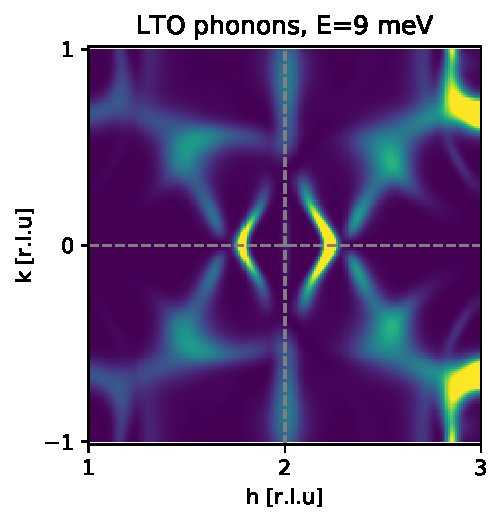
\includegraphics[width=0.45\textwidth]{fig/simulation/qxqy_neutron.pdf}
	\hspace{2em}
	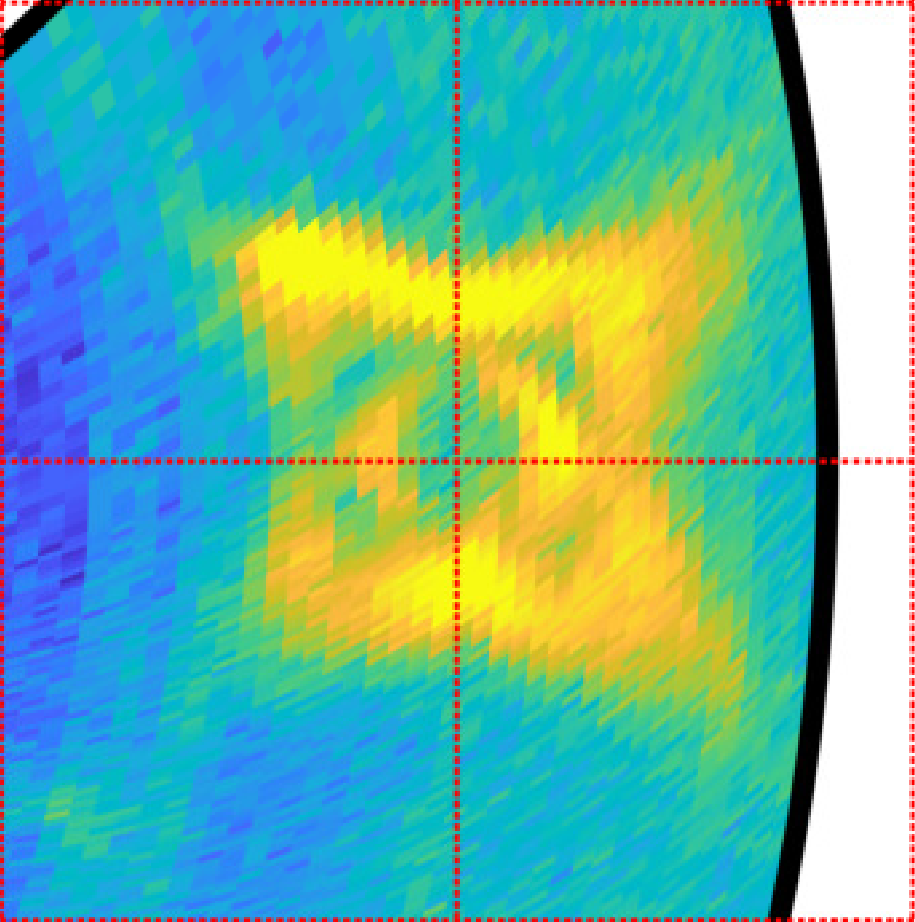
\includegraphics[width=0.45\textwidth]{fig/simulation/flatcone_data.png}
	\caption[flatcone 9 meV compared to simulation]{Simulation of neutron intensities compared to flatcone data at 9 meV.}
	\label{fig:qxqy_neutron}
	
\end{figure}

\section{LSCO}

In order to dope with strontium, we chose an equivalent doping of LCO+O (assuming that each oxygen atom adds two holes which is disputed). We thus replace two lanthanum atoms with strontium. With the assumption that strontium atoms are randomly, homogeneously distributed, we chose two sites where the distance is maximized. Inspection of the 2x2x1 supercell reveals that there are 4 reasonable choices of which one is chosen at random. The distance between the Sr ions is roughly \SI{8.85}{\angstrom}





\chapter{Molecular Dynamics}\label{ch:md}
Using the lessons learned in the previous chapter and after a reasonably successful validation of simulations (see section \ref{sec:sim_validation}), we can use the computational parameters at a lower precision and perform Molecular Dynamics simulations in VASP. The purpose of this chapter is to discuss the computational details, outline the chosen defect structures and finally present how defects (interstitial or otherwise) modifies the structure and dynamics of the parent compound. While molecular dynamics simulations are unable to provide information about the phonon band structure directly, it is possible to extract the phonon DOS and other relevant dynamical information as outlined in section \ref{sec:method_md}. In order to distinguish the simulations, we use a similar notation as in the previous chapter, but with the option to add dopants: [HTT/LTO/LTT][m]+[Sr/O$_\text{i}$], where omitting the [m] refers to the AFM electronic structure. For example, LTOm+Sr refers to a calculation starting from orthorhombic (Bmab) symmetry, in the metallic phase, with added Sr dopant.

\section{Computational Details}
Since Molecular Dynamics simulations require a large number of SCF cycles, it is necessary to drastically reduce the precision of our simulation. In general, the most drastic approximation comes from only running the simulation at one $k$-point ($\Gamma$). Other parameters are benchmarked by small test runs of a couple hundred steps and then evaluating the computational resources/time available. In our case we end up with the following additional reductions in precision:

\begin{itemize}
	\item Planewave cut-off at the default: \SI{400}{\eV} (\texttt{ENCUT=400})
	\item Threshold for the SCF to stop reduced to \SI{e-5}{\eV} (\texttt{EDIFF=1E-5})
	\item A faster algorithm for electronic minimization (\texttt{ALGO=F})
	\item Projection operators calculated in real space (\texttt{LREAL=A})
\end{itemize}

We keep the \texttt{PREC} tag set to `Accurate', since changing to `Normal' resulted in convergence issues. In addition, we need to specify the temperature and type of ensemble (see section \ref{sec:method_md}). For all simulations, we run at $T=\SI{300}{\kelvin}$ (\texttt{TEBEG=300}) within the canonical (NVT) ensemble using the algorithm of Nos\'{e} with a Nos\'{e}-mass such that the temperature fluctuates with a frequency of roughly \SI{38}{\tera\hertz} (\texttt{SMASS=1}). In order to get reasonable statistics we run with a time step $\Delta t = \SI{2}{\femto\second}$ (\texttt{POTIM=2}) for a total of 21000 (\texttt{NSW=21000}) steps, corresponding to a simulation time of \SI{42}{\pico\second}. For the analysis, we discard the first \SI{2}{\pico\second} in order to let the system equilibrate.

For the initial structures where defects have been added, we perform a geometry optimization of the supercell in order to find a structural minimum from which to start the MD simulation. Due to the reduced symmetry (compared to the phonon calculations in chapter \ref{ch:simulation}) this is a fairly expensive computation, so we perform the optimization with the same parameters as the MD simulation, except that we increase the $k$-point mesh to $4 \times 4 \times 4$ and the SCF threshold to \SI{e-6}{\eV}. Similar to the phonon calculations, we use the conjugate gradient algorithm for this minimization.

\section{Octahedral tilts}\label{sec:md_tilts}
\begin{figure}
	\centering
	\begin{subfigure}{0.64\textwidth}
		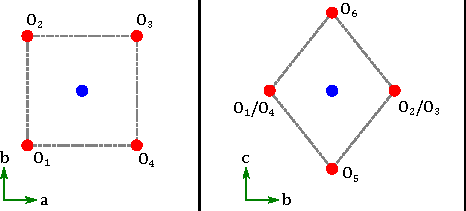
\includegraphics[width=\textwidth]{fig/md/q1q2_md_tilts.pdf}
	\end{subfigure}
	\begin{subfigure}{0.35\textwidth}
		\begin{align*}
			Q_1^1 &= \sin ^{-1} \left( \frac{O_6^x}{O_6^z} \right) \\
			Q_1^2 &= \sin ^{-1} \left( \frac{O_5^x}{O_5^z} \right) \\
			Q_1^3 &= \sin ^{-1} \left( \frac{O_1^z}{2 O_1^x} + \frac{O_2^z}{2 O_2^x} \right) \\
			Q_1^4 &= \sin ^{-1} \left( \frac{O_3^z}{2 O_3^x} + \frac{O_4^z}{2 O_4^x} \right)
		\end{align*}
	\end{subfigure}	
	\caption[Finding octahedral tilts from arbitrary oxygen positions]{Finding octahedral tilts from arbitrary oxygen positions. $Q_2$ angles can be found in an analogous way by replacing $x$ with $y$ and `pairing up' O$_1$ with O$_4$ and O$_2$ with O$_3$.}
	\label{fig:md_octahedral_tilts}
\end{figure}

In order to obtain octahedral tilts from MD simulations where symmetry is turned off, we are forced to define the octahedral tilts for each octahedra in the supercell. In fact, by writing which octahedra each oxygen atom (excluding interstitials) in our simulation belongs to, we can extract the $(Q_1,Q_2)$ tilt as seen from that oxygen. Since the tilts alternate, each tilt belongs to one of four symmetries with respect to $(Q_1,Q_2)$: (+,+), (+,-), (-,+), (-,-). In practice, we analyse the initial $t=0$ structure with the following steps for each Cu atom in the supercell:

\begin{enumerate}
	\item Record the position of the Cu atom
	\item Find apical oxygens by searching for (Cu, O) pairs with a distance less than $r = (1,1,2.7) \, \SI{}{\angstrom}$
	\item Find equatorial oxygens by searching for (Cu, O) pairs with a distance less than $r = (2.1,2.1,1) \, \SI{}{\angstrom}$
	\item Determine the $Q_1$, $Q_2$ tilt as seen from each of the 6 oxygen atoms in the list.
	\item Apply the symmetry operations.
	\item Save the 4 ($Q_1$, $Q_2$) value pairs.
\end{enumerate}

\noindent Step 4 is performed by first converting fractional coordinates to real-space coordinates and then finding angles as outlined in Figure \ref{fig:md_octahedral_tilts}. The symmetry operations in step 5 is a matrix with 8 columns corresponding to the 8 tilt values and a number of rows equal to the number of octahedra -- 16 in the case of our $2 \times 2 \times 1$ supercell. Each element of the matrix is either +1 or -1, where -1 will reverse the tilt direction and +1 will keep it as-is. The matrix can be generated by examining the output of the starting structure (which has the correct space group symmetry) and then constructing the matrix such that all $(Q_1, Q_2)$ tilts agree. While the same result can be archived by manually assigning the different atoms of our manageable supercell, this methodology allows the code to eventually be expanded to other systems, since we can set up arbitrary local coordinate systems.

After having performed this analysis, we can apply the same operations to every time step and obtain statistics about the time-evolution of the octahedral tilts in our system. This is similar to the Positional Recurrence Maps (PRM) methodology \cite{Piovano2016} that has been used to extract information about the apical oxygen dynamics in Nd$_2$NiO$_{4+\delta}$ \cite{Perrichon2015}.

\section{Structures with dopant ions}
Since the introduction of dopant ions breaks the crystal symmetry, we cannot perform phonon calculations using the direct method without making an excessive amount of high-precision calculations. Our typical $2 \times 2 \times 1$ supercell containing 112 ions with P1 symmetry would require $112 \times 3 = 336$ displacements just to describe phonon frequencies and eigenvectors at $\Gamma$. The worst case phonon calculation (LTT with magnetism) in the preceding chapter required just 21 displacements. For this reason, we are essentially forced to use molecular dynamics. In the following, the model for placing the initial dopants is outlined for Sr- and O-doped systems separately.

\subsection{LCO+O}
We start by considering the La$_2$CuO$_{4+\delta}$ System, which is simply LCO with added oxygen atoms at interstitial sites. It is generally accepted that the oxygen enters in the middle of the rock-salt layer, the least dense area of the crystal structure. Figure \ref{fig:oint_location} shows possible interstitial positions for the LTO (Bmab) and LTT (P4$_2$/ncm) phase, taken from a model proposed for the La$_2$NiO$_{4+\delta}$ system \cite{Tranquada1994}. Simulations in the defect phases are denoted by subscript `defect'. We ignore the HTT phase for molecular dynamics since the symmetry is broken and the preliminary geometry optimization would tend to tilt the octahedra similar to the LTT phase. To represent a reasonable doping level, we consider the addition of a single interstitial. It is generally accepted that the oxidation state is, at least approximately, O$^{2-}$, such that each dopant adds two holes. In our $2 \times 2 \times 1$ supercell with 16 formula units, this corresponds to a doping of $n_\text{h} = \frac{2}{16} = 0.125$.

\begin{figure}
    \centering
    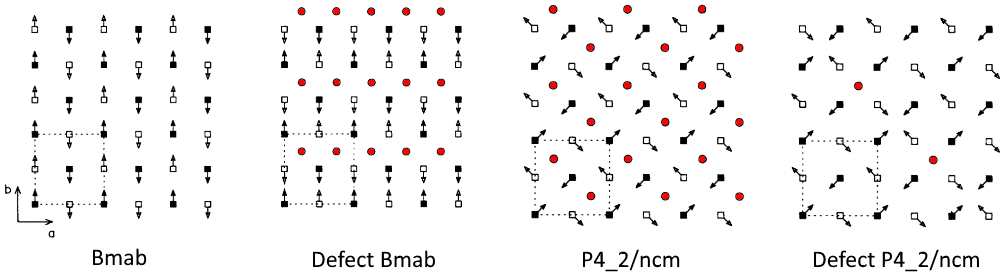
\includegraphics[width=\textwidth]{fig/md/oint.png}
    \caption[Illustration of interstitial positions]{Illustration of interstitial oxygen in-plane ($a$-$b$) location with respect to the apical oxygen displacements in the rock-salt layer. Open squares represent apical oxygens `hanging down' while closed squares represent apical oxygens `sticking up'. Interstitial oxygen are red circles and are shown on every possible interstitial site for clarity. Adapted from ref. \cite{Tranquada1994}.}
    \label{fig:oint_location}
\end{figure}

To see how the symmetry is broken, Table \ref{tab:oint_locations} shows the resulting space groups when inserting an interstitial into various starting symmetries. As expected, the symmetry is lowered substantially, especially if the $z$-component of the interstitial is different from $\frac{1}{4}$. While the symmetry isn't reduced to P1, it is difficult to imagine that any of the space groups in Table \ref{tab:oint_locations} could be used solve the observed superstructures in LCO+O (see section \ref{sec:lscoo}). Diffraction studies point to the interstitial being placed at either $\left(\frac{1}{4} \frac{1}{4} z \right)$ with $z$ close to $\frac{1}{4}$ or on a general $(xyz)$ position \cite{Rial1997}. When modelling this position in diffraction studies, it is possible to keep the parent symmetry by assigning an occupation factor to the interstitial and thus keeping the symmetry of the parent phase. Since we are not afforded that luxury when building structures for molecular dynamics, defects will naturally break the symmetry of our parent phase. Table \ref{tab:oint_locations} should thus not be seen as proposed models, but rather as an illustration of our inability to model partial occupancies in a small real-space box.

\begin{table}
	\centering
	\caption[Oxygen interstitial phases]{Space group symmetry due to the introduction of an interstitial oxygen in various structures all described in a $2 \times 2 \times 1$ supercell of the Bmab (conventional) coordinate system. HTT, LTO and LTT are the usual phases as described in literature \cite{Hucker2012}. The structures labelled defect is (1) in the LTO case: A stacking fault where the middle layer has its tilts reversed and (2) in the LTT case: A line along [110] with reversed tilts. Both are described in \cite{Tranquada1994} and are designed in order to `make room' for the interstitial oxygen (see Figure \ref{fig:oint_location}).}
    \label{tab:oint_locations}
    \begin{tabular}{@{}lllll@{}}
\toprule
Phase                   & Space Group & $\text{O}_\text{i}^x$ & $\text{O}_\text{i}^y$ & $\text{O}_\text{i}^z$ \\ \midrule
HTT                     & I4/mmm (139)      &         &         &         \\
HTT + O$_\text{i}$      & P-42m  (111)    & 0.125   & 0.125   & 0.25    \\
HTT + O$_\text{i}$      & Cmm2 (35)       & 0.125   & 0.125   & 0.24    \\
LTO                     & Bmab (64)       &         &         &         \\
LTO + O$_\text{i}$      & P2 (3)    & 0.125   & 0.125   & 0.25    \\
LTO + O$_\text{i}$      & P2 (3)         & 0.125   & 0.125   & 0.24    \\
LTO$_\text{defect}$     & Pmna (53)       &         &         &         \\
LTO$_\text{defect}$ + O$_\text{i}$ & P2 (3)         & 0.875   & 0.375   & 0.25    \\
LTO$_\text{defect}$ + O$_\text{i}$ & P2 (3)         & 0.875   & 0.375   & 0.24    \\
LTT                     & P4$_2$/ncm (138)  &         &         &         \\
LTT + O$_\text{i}$      & P-4 (81)        & 0.375   & 0.125   & 0.25    \\
LTT + O$_\text{i}$      & P2 (3)         & 0.375   & 0.125   & 0.24    \\
LTT$_\text{defect}$               & Pmma (51)       &         &         &         \\
LTT$_\text{defect}$ + O$_\text{i}$ & Cmm2 (35)       & 0.875   & 0.375   & 0.25    \\
LTT$_\text{defect}$ + O$_\text{i}$ & Cmm2 (35)       & 0.875   & 0.375   & 0.24    \\ \bottomrule
\end{tabular}

\end{table}

\subsection{LSCO}
In the La$_{2-x}$Sr$_x$CuO$_4$ system, our current best guess is that the distribution of the doped Sr species is completely random and homogeneous. Since randomness is difficult to implement in a (relatively) small system with periodic boundary conditions, we initially place them at a distance of about half the box side in order to  represent homogeneous doping. Replacing La$^{3+}$ with Sr$^{2+}$ adds one hole, so we add two dopants in order to be at $n_\text{h} = 0.125$ doping.

\section{Geometry Optimization}
We performed high-precision geometry optimizations of ionic positions only on these LCO+O defect structures starting from the various relevant symmetries. The starting structures were the optimized structures from chapter \ref{ch:simulation} with an interstitial inserted according to Table \ref{tab:oint_locations}. The defect structures were created by reversing certain tilts according to Figure \ref{fig:oint_location}. For the geometry optimization we kept the volume fixed at the value obtained from the parent structures without tilt defects, substitutions or interstitials. Performing an equation-of-state geometry optimization for all structures as in section \ref{sec:sim_geomopt} is computationally expensive for the defect supercells, but Figure \ref{fig:lcoo_eos} shows a EOS fit of the LTT structure with a limited number of points, revealing that the Volume does not change significantly due to the interstitial.

\begin{figure}
	\centering
	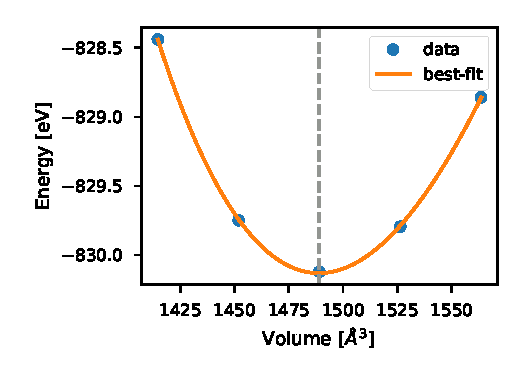
\includegraphics[width=0.6\textwidth]{fig/md/lcoo_eos.pdf}
	\caption[LCOO EOS]{Equation-of-state fit to La$_2$CuO$_{4.0625}$ starting from the LTT phase with one added interstitial oxygen in our supercell. The broken vertical line is the minimum of the fit, showing that our starting volume was reasonable. Each minimization was performed without symmetry while relaxing both ionic positions and the cell shape. The orthorhombic strain due to the cell shape change was below $\eta = 0.0004$ for all volumes, suggesting that the tetragonal crystal shape is a stable minimum.}
	\label{fig:lcoo_eos}
\end{figure}

Table \ref{tab:oint_lcoo_en} shows the resulting total energies and ($Q_1, Q_2$) tilts for a variety of starting structures including oxygen interstitials. A few trends emerge from this investigation. First, the defect structures in Figure \ref{fig:oint_location} has the effect of reducing the \emph{average} tilt of the structure, if we keep the symmetry operations from the non-defective phase. In the case of LTO the average tilts completely cancel out, while in the case of LTT they are cut in half. In addition, both the average and local tilts move towards the tilt pattern of the non-defective phase during optimization. In general, our simulations find that it costs more energy to reverse the tilts compared to the addition of the interstitial. This is inconsistent with the observation of staging (see section \ref{sec:lscoo}) and is likely related to the limited size of our simulation. Since a well-defined energy minimum is important for the initial configuration of the MD simulations, we stick with the parent, undistorted phases when investigating LCO+O. Finally, we notice that the tilts tend towards an `LTT-like' tilt-pattern in the optimization of metallic LTO, while keeping a significant orthorhombic strain. 

\begin{table}[b]
	\centering
	\caption[Oxygen interstitial phases: Energy]{Oxygen interstitial phases, geometry optimization. Geometry optimization performed on ionic positions only. $E_0$ corresponds to the energy after inserting the interstitial oxygen, but before geometry optimization. $E_1$ is the total energy after optimization. The octahedral tilts ($Q_1, Q_2$) are similarly defined before and after the optimization.}
	\label{tab:oint_lcoo_en}
	\begin{tabular}{llllll}
    \toprule
	 & $E_0$ [eV] & $E_1$ [eV] & $(Q_1, Q_2)_0$ & $(Q_1, Q_2)_1$  \\ 
	\midrule
    HTT + O$_\text{i}$                    & -827.27669             & -829.76250 & (0.00, 0.00) & (1.00, 1.00) \\
    LTO + O$_\text{i}$                    & -828.29890             & -830.39658  & (0.00, 5.79) & (1.21, 5.92) \\
    LTO$_\text{defect}$ + O$_\text{i}$            & -823.09516             & -830.03588  & (0.00, 0.00) & (2.12, 4.48) \\
    LTT + O$_\text{i}$                    & -828.04663             & -830.08248  & (4.61, 4.61) & (3.77, 3.72) \\
	LTT$_\text{defect}$ + O$_\text{i}$             & -826.03173             & -829.94243  & (2.31, 2.31) & (2.80, 2.70) \\
	LTOm + O$_\text{i}$                & -872.73074             & -876.56079  & (0.00, 6.42) & (3.76, 3.90) \\
	LTTm + O$_\text{i}$                & -872.35546             & -876.56195  & (4.53, 4.53) & (3.85, 3.85) \\
	\bottomrule
    \end{tabular}
\end{table}

Table \ref{tab:oint_lsco_en} shows the same optimizations performed on Sr-doped La$_2$CuO$_4$. The results here are as we expect from the small difference between the ionic radius of La$^{3+}$ and Sr$^{2+}$ (see table \ref{tab:dopants}). We seem to be in a well-defined minimum and the average tilt is only modified slightly. While geometry optimizations are only able to locate a local minimum, the results in Tables \ref{tab:oint_lcoo_en} and \ref{tab:oint_lsco_en} point toward the expected conclusion that interstitial oxygen has a more significant effect on the octahedral tilt patterns compared to Sr doping. The nature of these effects cannot be obtained from geometry optimizations alone, and we turn to molecular dynamics for the detailed analysis of structure and dynamics.

\begin{table}[b]
	\centering
	\caption[Sr doped phases: Energy]{Sr doped phases, geometry optimization. $E_0$ corresponds to the energy after replacing La with Sr, but before geometry optimization. $E_1$ is the total energy after optimization. Geometry optimization performed on ionic positions only. The octahedral tilts are similarly defined before and after the optimization.}
	\label{tab:oint_lsco_en}
	\begin{tabular}{lllll}
    \toprule
	 & $E_0$ [eV] & $E_1$ [eV] & $(Q_1, Q_2)_0$ & $(Q_1, Q_2)_1$  \\ 
	\midrule
    LTO + Sr                  & -858.73485             & -859.48650  & (0.00, 5.79) & (0.00, 5.38) \\
	LTOm + Sr                    & -858.57712             & -859.39905  & (0.00, 6.42) & (0.00, 5.69) \\
	LTT + Sr                    & -858.68994            & -859.49712  & (4.61, 4.61) & (3.87, 3.97) \\
	LTTm + Sr                    & -858.57810           & -859.40170  & (4.53, 4.53) & (3.98, 4.08) \\
	\bottomrule
    \end{tabular}
\end{table}

\section{Benchmarking}
Similar to our phonon calculations in the previous chapter, molecular dynamics simulations are typically benchmarked in various ways. Depending on the type of ensemble and thermostat, either the temperature or total energy is expected to be conserved. It is, however, possible for numerical noise to cause these quantities to drift. In our case the Nos\'{e} thermostat controls temperature through velocities, so it can be useful to plot the temperature as a function of simulation time to see if the fluctuations are reasonable. The temperature can be calculated from the MD trajectory by first computing the velocities through the Verlet algorithm (see section \ref{sec:method_md}) and then evaluating
%
\[ T = \frac{1}{3 k_\text{B} (N_\text{ions}-1)} \sum_j M_j |\bm{v}_j|^2 \, , \]
%
where $N_\text{ions}$ is the number of atoms, $M_j$ is the mass of atom $n$ and $\bm{v}_j$ is the velocity of atom $j$. We divide by $(N_\text{ions} - 1)$ rather than $N_\text{ions}$, since temperature is defined with respect to degrees of freedom and we can arbitrarily redefine our coordinate system with respect to a particular atom. When considering the instantaneous temperature in this way, we expect the mean-squared temperature fluctuations to be \cite{Hickman2016}
%
\[ \left\langle \left( \Delta T^2 \right) \right\rangle = \frac{2T_0^2}{3N_\text{ions}} \, . \]
%
Four our simulation with $N_\text{ions} = 112$ at $T_0 = \SI{300}{\kelvin}$ we thus expect temperatures fluctuations of $\pm \SI{23.15}{\kelvin}$. Figure \ref{fig:stitch} is a summary of benchmarks performed on the LCO in the LTO phase with no dopant ions or defects. Simulations were performed with two different time steps and the difference in temperature fluctuations and the resulting phonon DOS was recorded. In terms of temperature fluctuations, there is little effect of going from 1 to 2 fs time steps, but there are slight modifications to the DOS, especially in the region around 30 meV. While this may be seen as problematic, it is important to realize that we are probing a relatively small number of steps, and it is unlikely that our simulation is completely ergodic. In other words, we may be probing a different area of phase space in the two simulations. It is unlikely that the time step resolution itself is causing the effects on DOS, since an energy of \SI{30}{\milli\eV} = \SI{7.3}{\tera\hertz} is probed by simulation times of roughly \SI{137}{\femto\second}. While higher precision is always desirable, we stick with a time step of \SI{2}{\femto\second} in order to be able to probe dynamics for longer time scales in more systems. Now, almost by definition, different time steps do probe different dynamics. I emphasize that any comparison between MD simulations is done at the same time step.

\begin{figure}
	\centering
	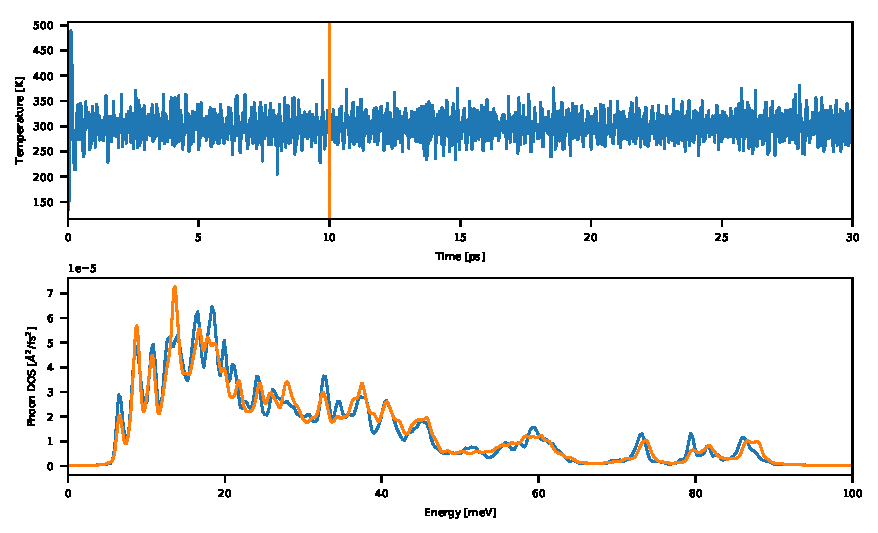
\includegraphics[width=\textwidth]{fig/md/stitch.pdf}
	\caption[stitched md runs]{Benchmark of molecular dynamics, using LCO in the LTO phase with no dopant ions or defects. \textbf{Top:} Temperature fluctuations for a simulation stitched together with the first \SI{10}{\pico\second} using a \SI{1}{\femto\second} time step and the last part of the simulation using a \SI{2}{\femto\second} time step. \textbf{Bottom:} Density of States weighted by neutron-cross sections and broadened by a Gaussian with $\sigma=\SI{0.5}{\milli\eV}$ (\SI{1.18}{\milli\eV} FWHM) evaluated at the same two parts of the simulation.}
	\label{fig:stitch}
\end{figure}

\section{DOS and PDF}
Molecular dynamics simulations have been performed with 7 starting configurations based on geometry optimizations in Table \ref{tab:oint_lcoo_en} and \ref{tab:oint_lsco_en} as well as references without dopant ions. Since the full matrix of combinations now includes 3 structural phases, 2 dopant ions, 2 electronic phases and 2 `defect' phases, the total number of desired simulations is 20. In order to limit the scope and focus computational resources, we chose to focus on the LTO phase and end up with the following list of simulations:

\begin{enumerate}
	\item LTT: LTT in AFM phase.
	\item LTO: LTO in AFM phase.
	\item LTO+Sr: LTO in AFM phase with added Sr dopants.
	\item LTO+O: LTO in AFM phase with added O dopant.
	\item LTOm: LTO in metallic phase.
	\item LTOm+Sr: LTO in metallic phase with added Sr dopants.
	\item LTOm+O: LTO in metallic phase with added O dopant
\end{enumerate}

Our primary observables when comparing to experiment is the phonon density of states and pair-density-function. We start by considering the DOS of all simulations, calculated with the method described in section \ref{sec:method_md} and the scripts developed in appendix \ref{app:software}. Figure \ref{fig:lto_md_defect_comparison} shows the neutron-weighted phonon DOS for all 7 simulations. While the overall shape of the phonon DOS is mostly unchanged, there are some subtleties that we might consider for further analysis. For the magnetic simulations, we see a similar modification of modes at $\approx \SI{30}{\milli\eV}$ when comparing the LTO and LTT phases. Interestingly, the sharp dip in DOS at \SI{30}{\milli\eV} is seen in LTO+O as well. In fact, the LTT and LTO+O phases appear to share more qualitative features with each other compared to the parent LTO phase. This is consistent with the initial geometry optimization of LCO+O in table \ref{tab:oint_lcoo_en} moving towards a LTT-like tilt pattern. LTO+Sr, on the other hand, mostly seem to broaden features rather than directly modify then. 

For the metallic simulations, we see similar trends but in a much more smeared out fashion, possibly due to reduced accuracy of these simulations due to the fermi surface smearing (see figure \ref{fig:sim_bench_para} in section \ref{sec:sim_benchmark}). Similar to the observations in chapter \ref{ch:simulation}, the main modification of the phonon DOS compared to the magnetic simulations is related to the high energy modes.

\begin{figure}
	\centering
	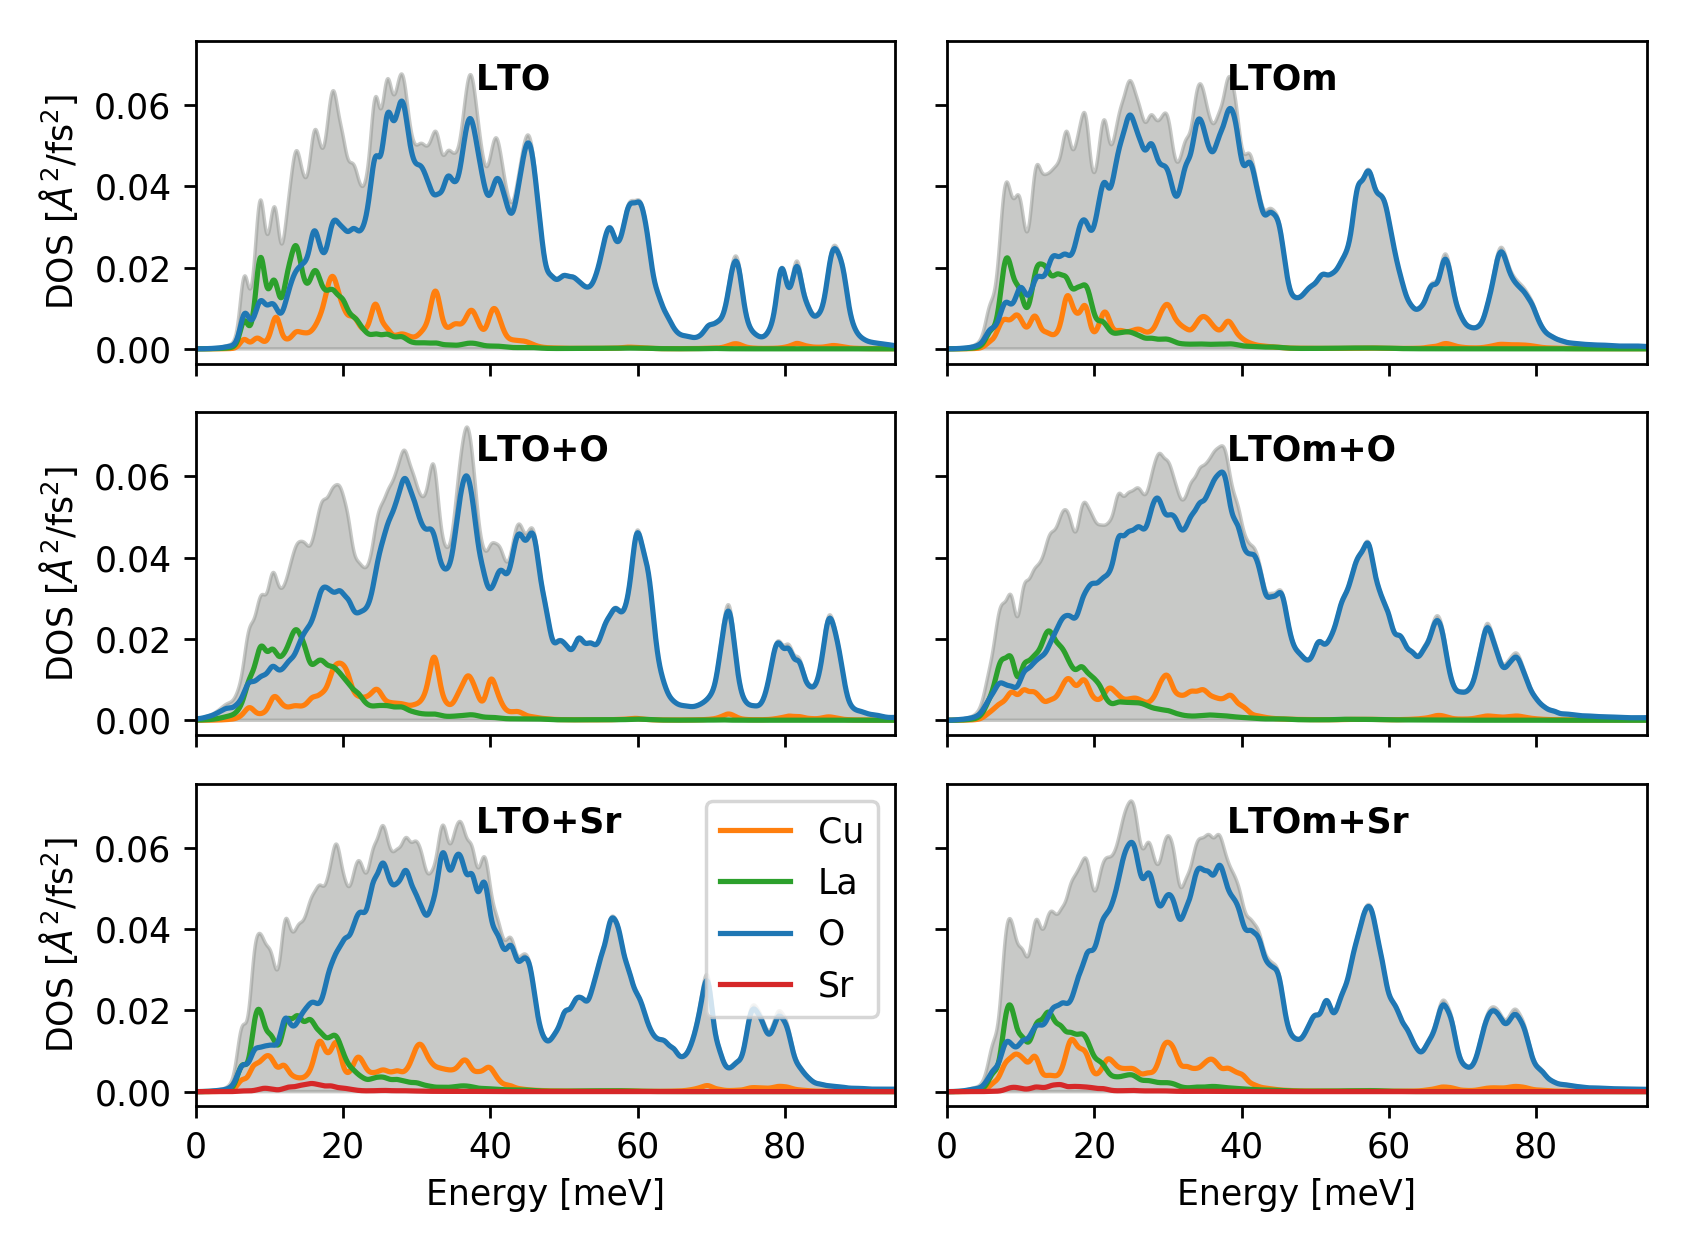
\includegraphics[width=\textwidth]{fig/md/lto_defect_comparison.png}
	\caption[LTO MD DOS: Defect comparison]{Neutron-weighed density-of-states for all molecular dynamics simulations performed in this chapter. The filled grey area is the total DOS and the lines are the partial atomic DOS. The initial conditions for the MD simulation is annotated on each plot according to the notation outlined in the beginning of this chapter. The density-of-states was obtained through the power spectrum of the velocity autocorrelation function (see section \ref{sec:method_md}). The power spectrum was smoothed by a Gaussian kernel with width $\sigma=\SI{0.5}{\milli\eV}$ (\SI{1.18}{\milli\eV} FWHM).}
	\label{fig:lto_md_defect_comparison}
\end{figure}

In order to compare more directly these observations, Figure \ref{fig:dos_pdf} shows a direct comparison of DOS and PDF of our LTO, LTO+O and LTT simulations. This comparison clearly shows that the LTT and LTO+O share common features especially around \SI{30}{\milli\eV} (various $c$-axis modes, see section \ref{sec:sim_dos} and \SI{60}{\milli\eV} (apical oxygen bond-stretching mode). The PDF in the same figure show only very subtle deviations, most notably around \SI{5.2}{\angstrom} where, once again, the LTT simulation shares features with LTO+O.

\begin{figure}
	\centering
	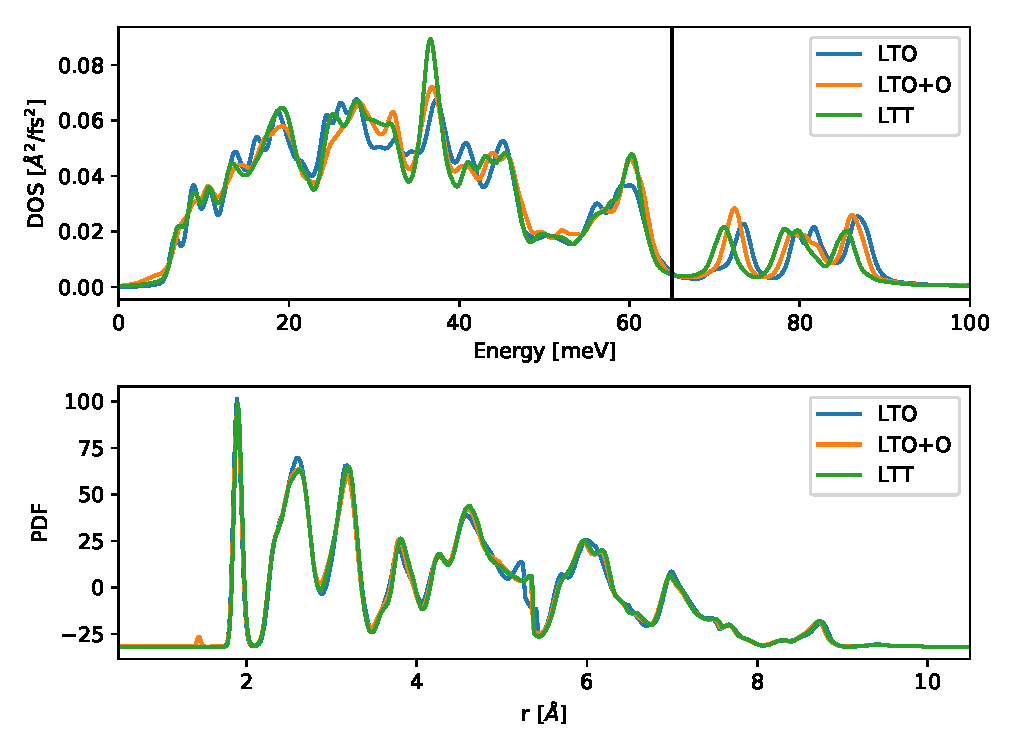
\includegraphics[width=\textwidth]{fig/md/lto_ltt_ltoo_comparison.pdf}
	\caption[MD: DOS and PDF]{\textbf{Top}: Total DOS for selected MD simulations. In general, differences are subtle, but we see some surprising similarities between the LTO+O and LTT simulation, indicating LTT-like behavior due to the interstitial (see text). \textbf{Bottom}: PDF of the same simulations, showing almost identical spectra for the 3 simulations. At roughly \SI{5.2}{\angstrom} there is a small modification where, once again, LTO+O and LTT simulations show similarities.}
	\label{fig:dos_pdf}
\end{figure}

\section{Microscopic analysis}
In addition to observables for comparison with experiment, the purpose of molecular dynamics simulations is to relate microscopic phenomena to these observables. For this reason, we will try to extract relevant information from the simulation trajectory in order to understand what is causing the changes in the phonon DOS and PDF. In the cuprates, there is much experimental evidence of the fact that Cu-O distances and distributions are important for superconductivity \cite{Bozin2000, Peng2017, Ivashko2019}. Inspired by these results, Figure \ref{fig:md_distances} show the distribution of Cu-O$_\text{equatorial}$ and Cu-O$_\text{apical}$ distances for selected simulations. In general, they follow a normal distribution showing that the harmonic approximation works well for our system, with the notable exception of the apical oxygen distance in LTO+O. 

\begin{figure}
	\centering
	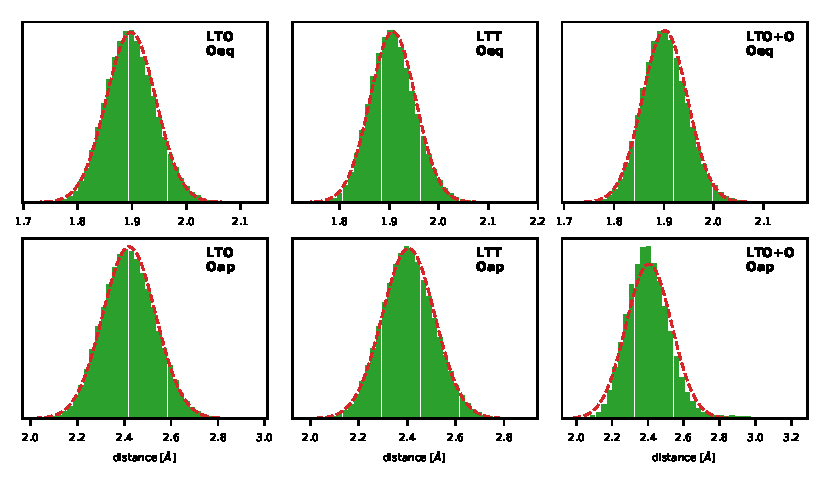
\includegraphics[width=\textwidth]{fig/md/dist_hist.pdf}
	\caption[MD: distance histograms]{Distance histograms of Cu-O distances with respect to the equatorial oxygen (Oeq) and apical oxygen (Oap) in the three simulations we compared in Figure \ref{fig:dos_pdf}. The data was generated by recording all appropriate distances at every time step of the simulation. The $y$-axis is normalized to unity and the broken line is a Gaussian function with expected value and variance calculated from the data. The histograms are normalized to unity.}
	\label{fig:md_distances}
\end{figure}

Table \ref{tab:md_cu_o_distances} summarizes these distances for all of the performed simulations. As expected from the almost identical PDF across simulations, the mean Cu-O$_\text{equatorial}$ distances does not seem to have any discernible trends, but there is a slight widening of the distributions in the systems containing dopants. In some sense this is expected since we have created different local environments by the introduction of impurity dopants. The same trend can be seen in the Cu-O$_\text{apical}$ distanced, but here we additionally have an shortening of the mean distance due to the introduction of oxygen (notice also that this shortening is identical to the LTT distance in magnetic case). For Sr-doping there is an elongation in the magnetic simulation but a shortening in the metallic simulation. It is, however, important to note that these differences are extremely subtle and may just be due to numerical peculiarities.

\begin{table}
	\centering
	\caption{Cu-O Distances distance statistics for all MD simulations performed in this chapter. Columns 2 and 3 show the mean distance and standard deviation for the Cu-O equatorial distance. Column 3 is the $R^2$ value of a linear regression assuming a normal distribution. Columns 4-6 show the same values for the Cu-O apical distance.}
	\label{tab:md_cu_o_distances}
	\begin{tabular}{lllllll}
		\toprule
			name &   $\langle \text{O}_\text{eq} \rangle $ [\AA]  & $\sigma$ (O$_\text{eq}$) [\AA] &  $R^2$ (O$_\text{eq}$) & $ \langle \text{O}_\text{ap} \rangle$ [\AA] & $\sigma$ (O$_\text{ap}$) [\AA] &  $R^2$ (O$_\text{ap}$) \\
		\midrule
			 LTO &  1.898 &  0.0455 &  0.9972 &  2.421 &   0.113 &  0.9989 \\
		   LTO+O &  1.902 &  0.0464 &  0.9972 &  2.406 &   0.127 &  0.9608 \\
		  LTO+Sr &  1.898 &  0.0507 &  0.9947 &  2.438 &   0.146 &  0.9995 \\
			LTOm &  1.909 &  0.0514 &  0.9951 &  2.462 &   0.140 &  0.9997 \\
		  LTOm+O &  1.908 &  0.0532 &  0.9934 &  2.440 &   0.156 &  0.9992 \\
		 LTOm+Sr &  1.905 &  0.0523 &  0.9947 &  2.451 &   0.151 &  0.9992 \\
			 LTT &  1.907 &  0.0461 &  0.9971 &  2.406 &   0.109 &  0.9992 \\
		\bottomrule
		\end{tabular}
\end{table}

Using the definitions of octahedral tilts described in section \ref{sec:md_tilts}, Figure \ref{fig:md_q1_q2_all} shows a histogram of $(Q_1, Q_2)$ tilts from all of our performed MD simulations on a logarithmic scale. Similar to observations from DOS and PDF, the tilt patterns of LTO+O are LTT-like, while the Sr-doped and parent compounds have tilts distributed around $(Q_1, Q_2) = (0,5)$ which is the equilibrium LTO structure. We also notice that the LTT-like simulations (LTT, LTO+O, LTOm+O) are able to transition between the  symmetrically equivalent tilt patterns, while the LTO-like simulations are `stuck' in the initial configuration. This is an indication that LTT-like tilts have distinct dynamics compared to LTO-like tilts.

\begin{figure}
	\centering
	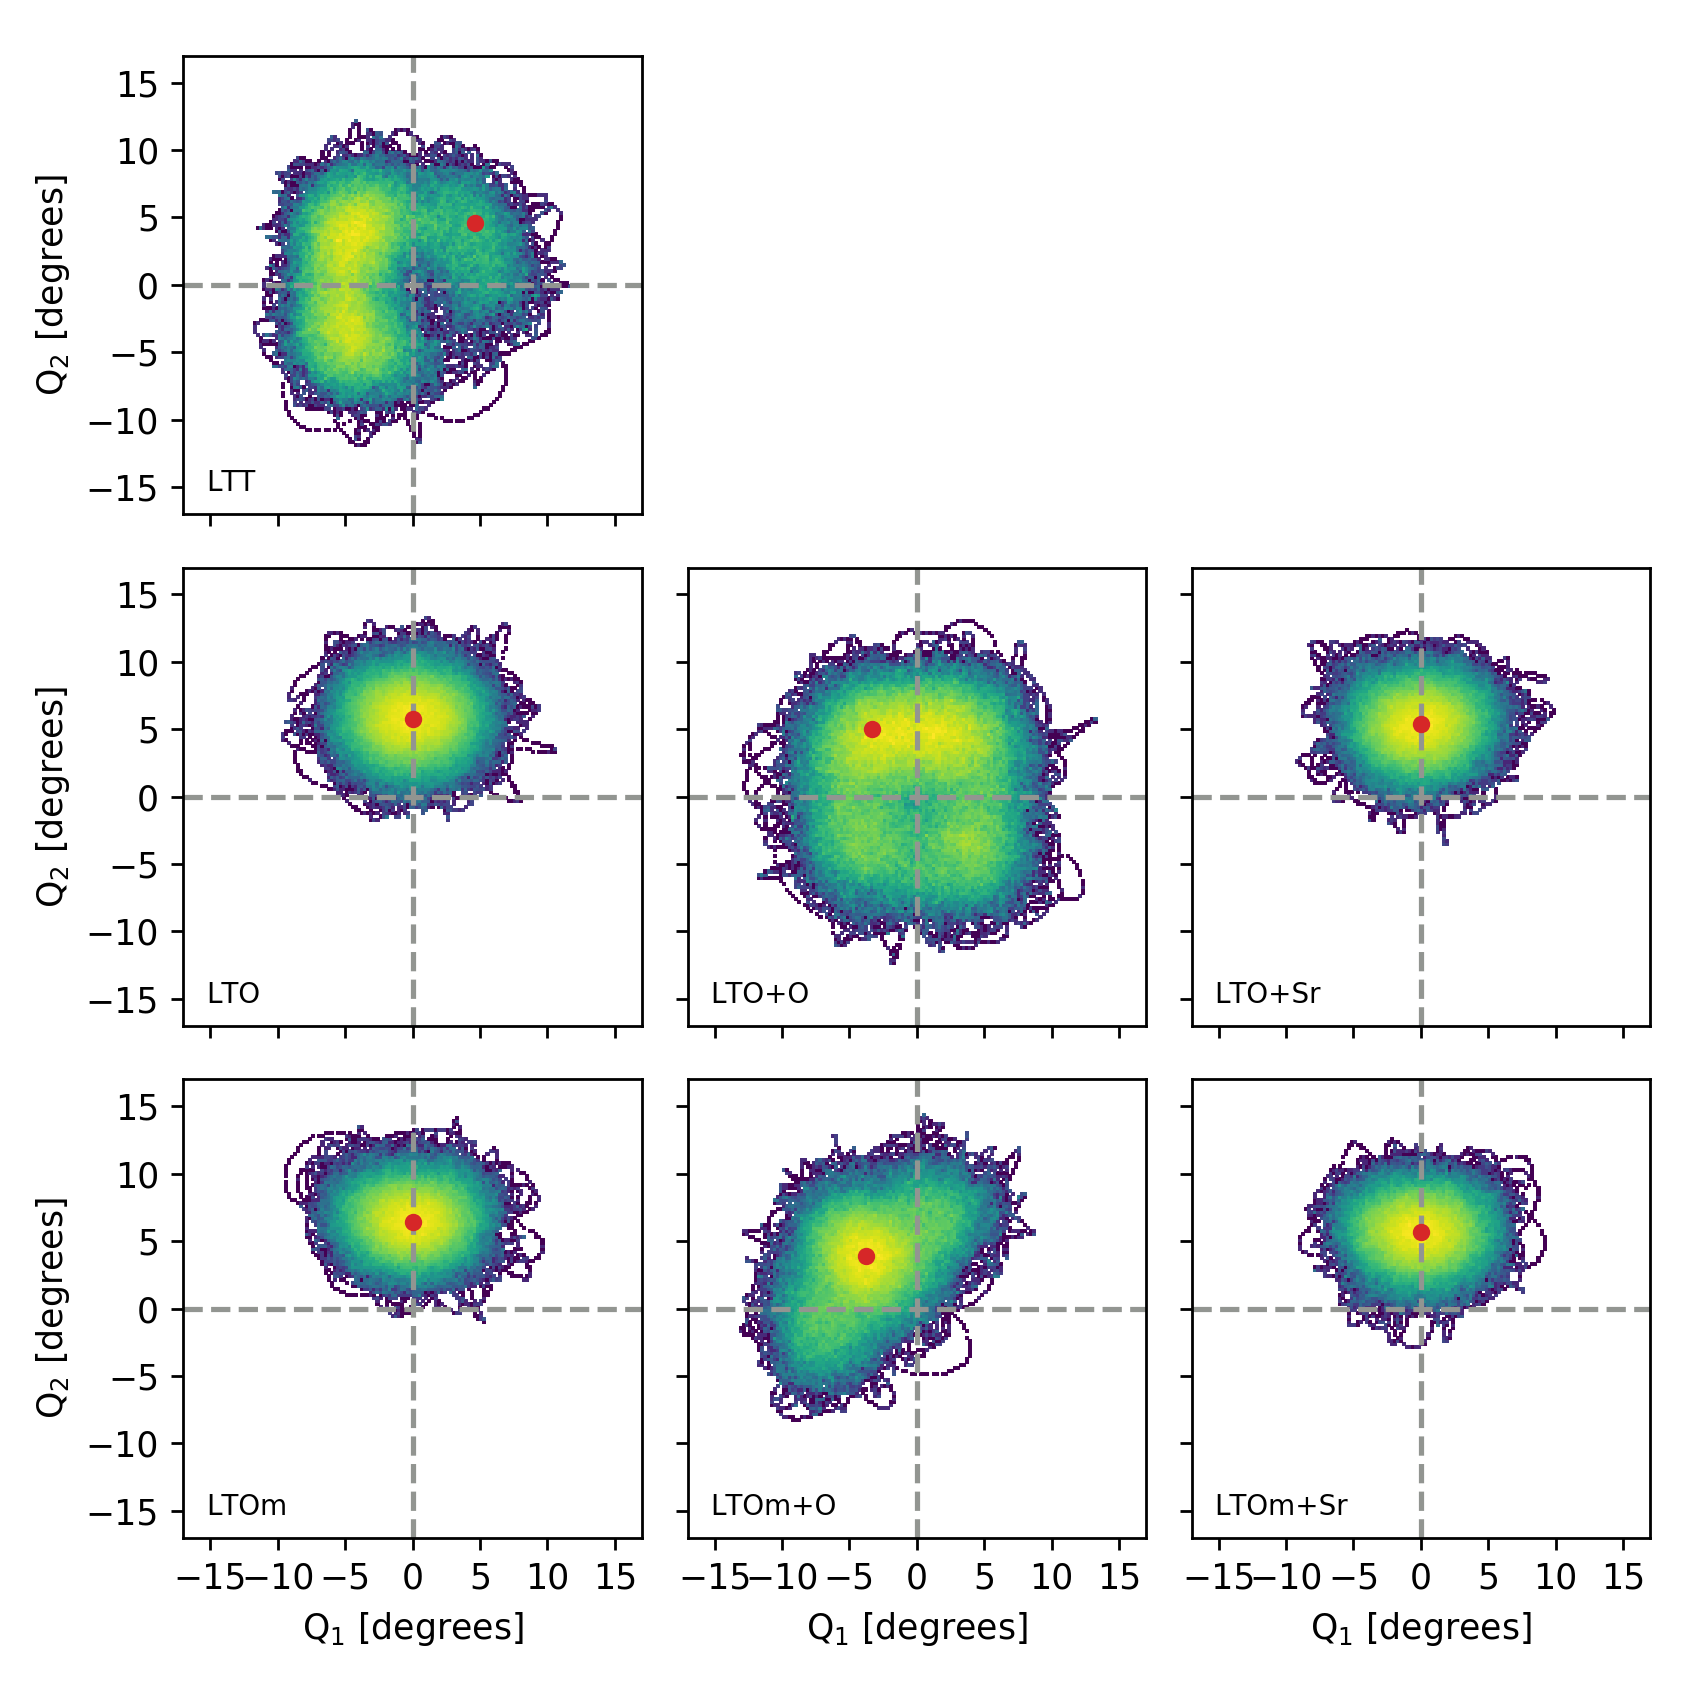
\includegraphics[width=\textwidth]{fig/md/Q1_Q2_all.png}
	\caption[MD Q1 Q2 All sims]{Tilt histograms of all performed molecular dynamics simulations. Plots are generated by obtaining the tilt as seen from apical oxygens and pairs of equatorial oxygens (as described in section \ref{sec:md_tilts}) for each time step and then plotting a 2D histogram of the resulting data on a logarithmic scale. The red circle denotes the starting tilt. As discussed in the text, we distinguish between LTT-like tilts sitting on the diagonals of this figure and LTO-like tilts sitting along the main axes. The same symmetry operations are applied at each time step, such that transitions between symmetrically equivalent configurations is visible in this plot.}
	\label{fig:md_q1_q2_all}
\end{figure}

Finally, figures \ref{fig:md_diffusion1} investigates the dynamics of the placed interstitial in LTO+O by following the in-plane location of the interstitial by plotting a histogram of its location as well as a line depicting its time evolution at equally spaced points in time. Additionally, we plot the $c$-axis evolution with a 1d histogram. For contrast, Figure \ref{fig:md_diffusion3} shows the same plots for a `normal' apical oxygen. Finally, Figure \ref{fig:md_diffusion2} shows the distribution of the apical oxygen near the interstitial, revealing a very similar distribution. These figures together show that the interstitial forms a `binary system' with the closest apical giving rise to a very localized effect. At $T=\SI{300}{\kelvin}$ we thus see no indication of diffusion. In some sense this is not surprising since diffusion is likely slow and not accessible within our relatively short \SI{40}{\pico\second} simulation times. In fact, the estimated `annealing time' for La$_2$CuO$_{4+\delta}$ has been estimated to be one week at room temperature \cite{Lee2004} (1 week divided by \SI{40}{\pico\second} is roughly $10^16$).

\begin{figure}
	\centering
	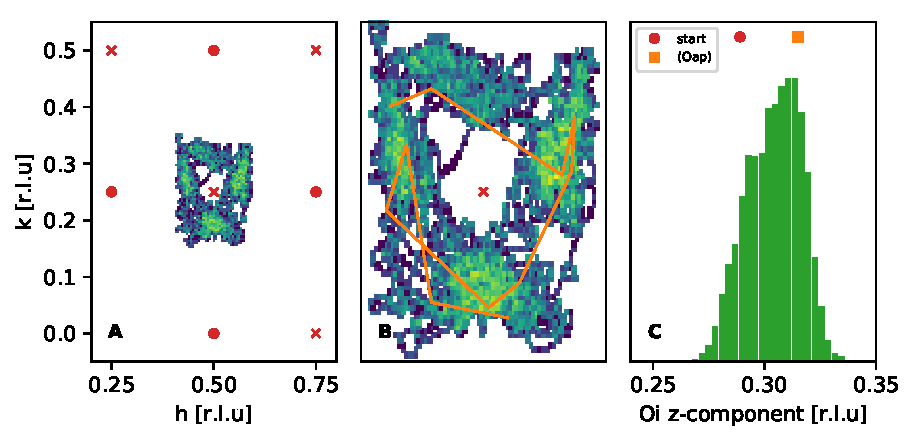
\includegraphics[width=\textwidth]{fig/md/diffusion1.pdf}
	\caption[MD Oint Diffusion Oi]{Distribution of the interstitial oxygen in LTO+O. \textbf{(A)}: In-plane distribution of the interstitial. Circles denote apical oxygens `sticking up', while crosses denote apical oxygen `hanging down' (similar to Figure \ref{fig:oint_location}). \textbf{(B)}: Zoomed-in version of \textbf{(A)} with the line marking the time-evolution of the interstitial sampled at isochronal points. \textbf{C}: $c$-coordinate distribution of the interstitial with the initial and average position marked in red and orange, respectively.}
	\label{fig:md_diffusion1}
\end{figure}

\begin{figure}
	\centering
	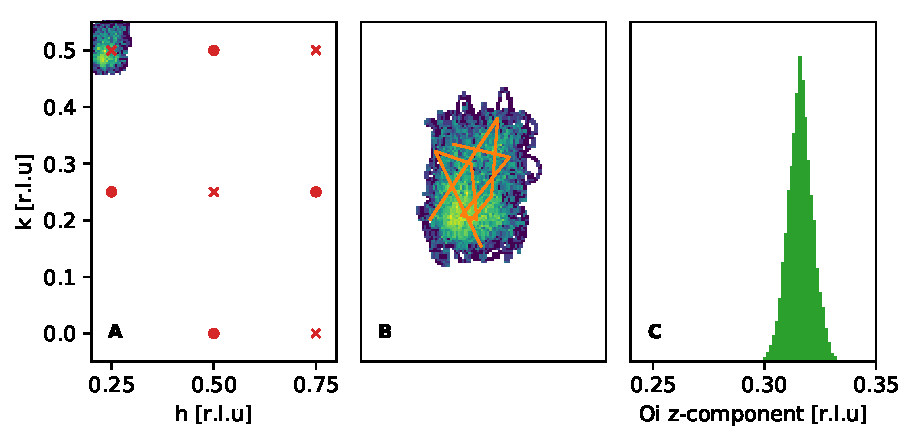
\includegraphics[width=\textwidth]{fig/md/diffusion3.pdf}
	\caption[MD Oint Diffusion Oap 2]{Distribution of a normal apical oxygen in LTO+O. \textbf{(A)}: In-plane distribution of the apical. Circles denote apical oxygens `sticking up', while crosses denote apical oxygen `hanging down' (similar to Figure \ref{fig:oint_location}). \textbf{(B)}: Zoomed-in version of \textbf{(A)} with the line marking the time-evolution of the interstitial sampled at isochronal points. \textbf{C}: $c$-coordinate distribution of the apical.}
	\label{fig:md_diffusion3}
\end{figure}

\begin{figure}
	\centering
	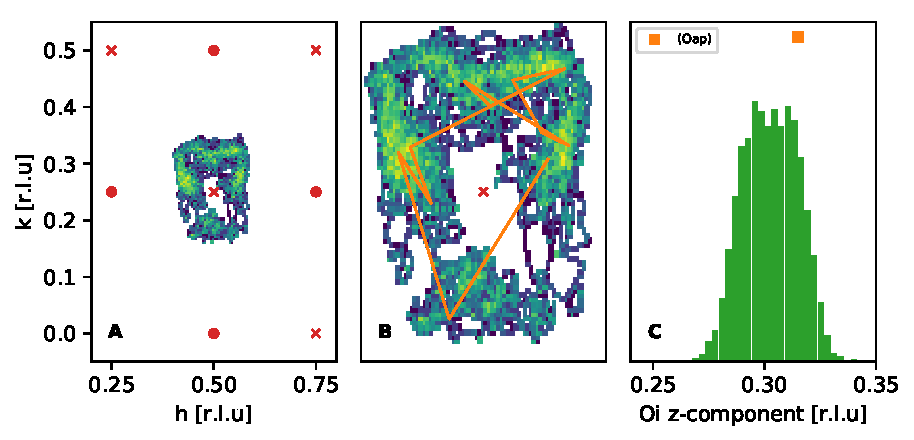
\includegraphics[width=\textwidth]{fig/md/diffusion2.pdf}
	\caption[MD Oint Diffusion Oap 1]{Distribution of an apical oxygen in LTO+O near the interstitial. \textbf{(A)}: In-plane distribution of the apical. Circles denote apical oxygens `sticking up', while crosses denote apical oxygen `hanging down' (similar to Figure \ref{fig:oint_location}). \textbf{(B)}: Zoomed-in version of \textbf{(A)} with the line marking the time-evolution of the interstitial sampled at isochronal points. \textbf{C}: $c$-coordinate distribution of the apical, with the average position marked in orange.}
	\label{fig:md_diffusion2}
\end{figure}

\section{Summary}
The main take-home message from chapter is the fact that interstitials seem to have a very subtle effect on structure but a more significant effect on dynamics. In particular, an observable such as PDF will se barely any difference between our simulations but high-quality DOS measurements should be able to see subtle differences due to dopants.

If we can obtain a reasonable validation of these simulations, the microscopic analysis reveals very clearly that oxygen interstitial phases move towards LTT-like tilt dynamics. Since the average structure of LCO+O at accessible temperatures is LTO, a possible explanation is that this tendency toward LTT-like tilts can result in the observed superstructures (and/or staging) \cite{Ray2017,Fratini2010} if we had access to bigger simulation boxes and longer simulation times. It might be valuable to examine this more closely with real-space methods such as reverse monte-carlo (RMC) or by performing classical MD based on the results obtained in this chapter.

Before moving on to experimental comparisons, Figure \ref{fig:md_phonopy_comparison} shows a comparison of phonon DOS as calculated from the previous chapter and the one obtained from molecular dynamics here. While there is a definite distinction between the spectra, it is important to realize that they are obtained by very different methods, while being based on the same computational background. In addition, molecular dynamics are not constrained by symmetry.

A direct comparison between molecular dynamics and phonon calculations should thus only be performed with extreme caution. For this reason, we mainly use the phonon calculations to identify the kinds of bands that correspond to certain features in the phonon DOS. When analyzing the role of dopants, simulations will all be done in the context of molecular dynamics (e.g. figure \ref{fig:dos_pdf}). In the experimental chapters I will leverage the phonon band structure calculations in context of triple-axis measurements of single crystals. Molecular dynamics simulations, on the other hand, will be used in the context of PDF and inelastic time-of-flight measurements of powdered samples.


\begin{figure}
	\centering
	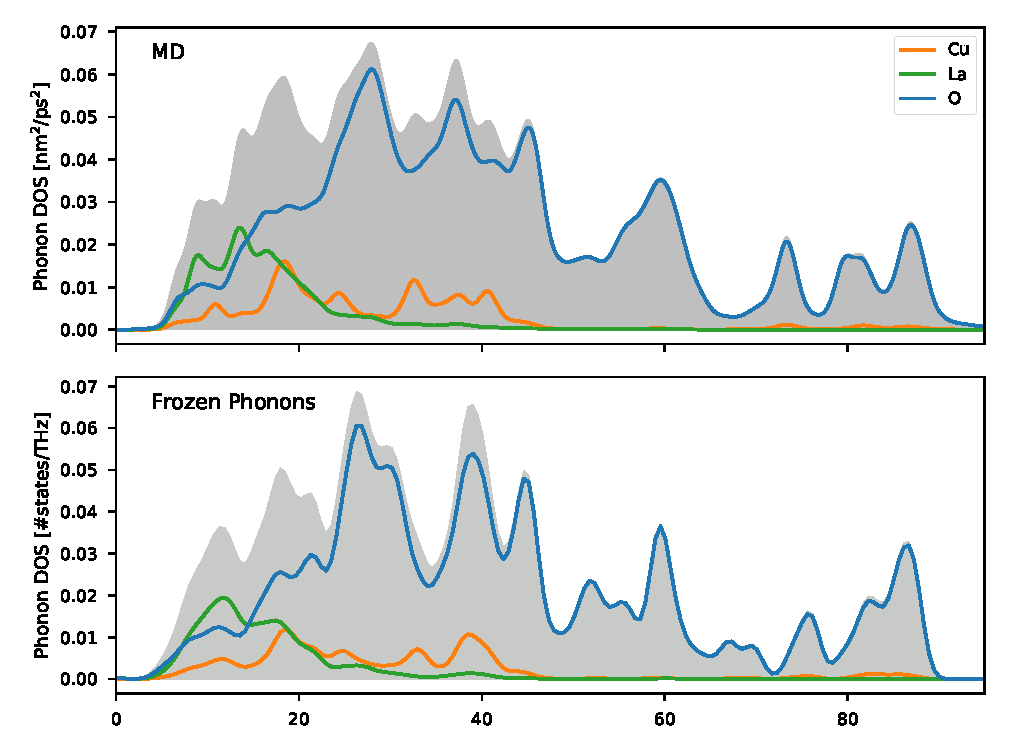
\includegraphics[width=\textwidth]{fig/md/md_phonopy_comparison.pdf}
	\caption[MD Phonopy Comparison]{Comparison of neutron-weighted phonon density of states obtained from \textbf{top:} the velocity autocorrelation function of a molecular dynamics trajectory and \textbf{bottom:} by integration of phonon bands calculated using the direct method (see chapter \ref{ch:simulation}). Both simulations are based on the low-temperature orthorhombic (LTO) structural phase.}
	\label{fig:md_phonopy_comparison}
\end{figure}



\chapter{Local structure of LSCO+O}\label{ch:local}
In this chapter, we look at structural correlations in La$_{2-x}$Sr$_x$CuO$_{4+\delta}$ (LSCO+O) containing oxygen interstitials. As discussed in section \ref{sec:lscoo}, LSCO+O is known to form complex superstructures that shows up in single-crystal diffraction. To quickly recap, `staging' \cite{Wells1997,Ray2017} was discovered early on and appears unrelated to superconductivity. On the other hand, novel superstructures, known as `Local Lattice Distortions' (LLD) and `Oxygen Interstitials' (O$_\text{i}$), are suggested to have a connection with superconductivity \cite{Poccia2011}. In fact, it appears that these two orderings are anti-correlated in real space, forming `puddles' on \SI{}{\micro\meter} scale \cite{Poccia2012}.

The data shown in this chapter is a collection of experiments performed on three different instruments: IN8, ThALES and D4 at Institut Laue-Langevin\todo{what is the best way to cite the instruments?} in Grenoble, France. In the first part, we explore some of the superstructures mentioned above in two single crystals of LSCO+O: La$_2$CuO$_{4+\delta}$ ($T_\text{c} = \SI{43}{\kelvin}$) and La$_{1.94}$Sr$_{0.06}$CuO$_{4+\delta}$ ($T_\text{c} = \SI{37.5}{\kelvin}$). In the second part, we perform a diffraction experiment on powders of LSCO+O with the purpose of looking at real space correlation through pair-distribution-function (PDF) analysis.

\section{Superstructures in single crystals}\label{sec:single_crystal_superstructures}
While superstructures in LSCO+O have been extensively studied in the past, it is always useful to check if your samples comply with conventional logic. The measurements shown here were mostly performed as a reference for some of the work shown in chapter \ref{ch:lowen}, but I present it here since it has relevance for structural correlations and can help us with the analysis of the PDF data in the following section. Superstructures in LCO+O are generally observed at $Q_2 = (0, 0.21, 0.29)$ and $Q_3 = (0.09, 0.24, 0.50)$ \cite{Kusmartsev2000} and should thus mainly be observable in the $a$-$c$ (or equivalently $b$-$c$ due to twinning\todo{mention twinning in introduction}) plane.

When using certain Triple-Axis spectrometers (IN8, IN20, ThALES) at the ILL, we have the option of a secondary spectrometer (everything after the sample) called FlatCone \cite{flatcone} where we can probe a large part of reciprocal space simultaneously. In particular, the FlatCone analyser system is built in such a way that you probe a large part of the scattering plane at a constant energy transfer $\hbar\omega$. In the following we are interested in structural correlations, so we are measuring at $\hbar\omega = 0$. In chapter \ref{ch:lowen} we will investigate finite energy transfers in detail.

\begin{figure}
    \centering
    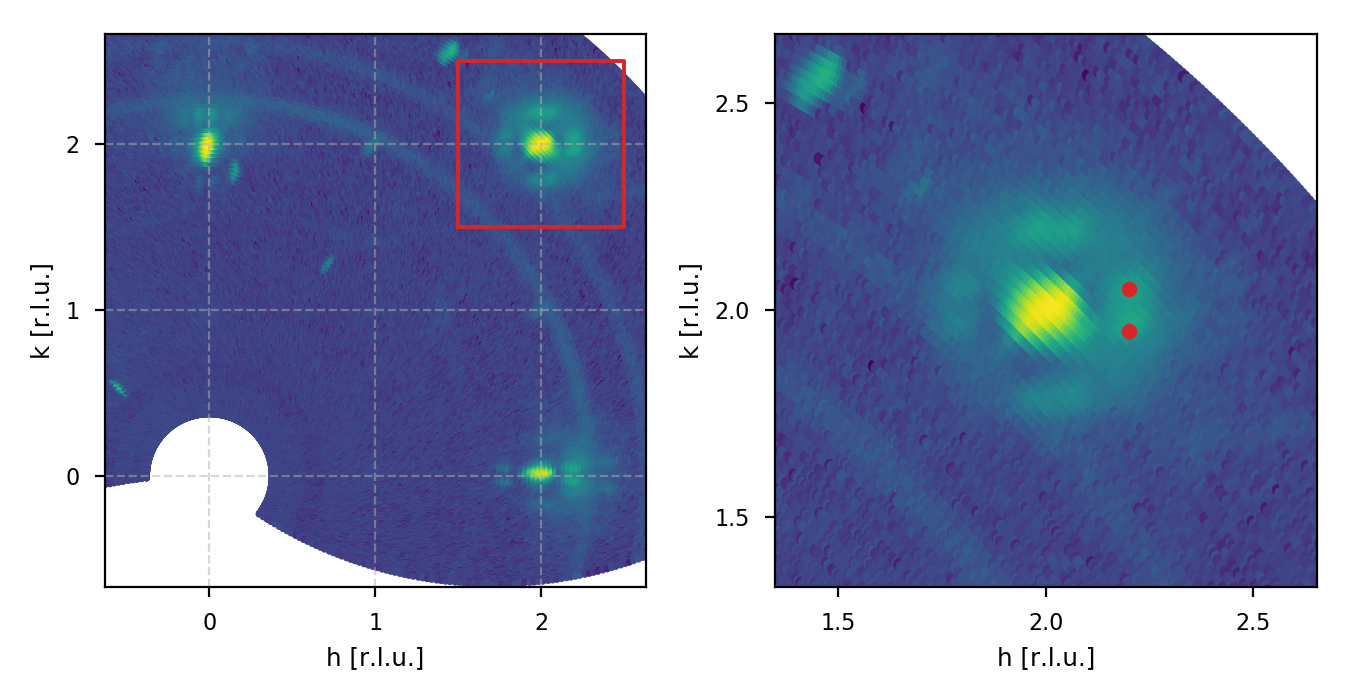
\includegraphics[width=0.9\textwidth]{fig/pdf/lcoo_ab_elastic.png}
    \caption{Reciprocal space map of single crystal La$_2$CuO$_{4+\delta}$, measured in the $a$-$b$ plane with the unconventional Bmab orthorhombic coordinate system. \textbf{Left}: Full map, showing mainly the fundamental Bragg peaks. Circular arcs are powder lines from Al. \textbf{Right}: Zoomed-in view of the are marked in red. We notice satellite peaks around (220) at $Q=(0.2,\pm 0.05,0)$ ($|Q| = \SI{0.241}{\per\angstrom}$).}
    \label{fig:lcoo_ab_elastic}
\end{figure}

Figure \ref{fig:lcoo_ab_elastic} shows the result of such a measurement of La$_2$CuO$_{4+\delta}$ on the thermal TAS IN8, performed in the $a$-$b$ plane using the orthorhombic coordinate system (see section \ref{sec:lscoo} in chapter \ref{ch:intro}\todo{maybe put a dedicated section in the introduction or simulation chapter}). The coverage of our measurement is such that we are see the (200), (020) and (220) fundamental Bragg peaks. While mostly unremarkable, some satellite peaks are visible at roughly $Q = (0.2, \pm 0.05, 0)$ as marked on the zoomed-in right-hand-side of the figure. Satellite peaks with zero $l$-component has been previously reported by our group \cite{Ray2016}, but the nature of these peaks are currently unknown. We can, however, make the simple observation that this peak corresponds to a real-space structural correlation with a length $d_1 \approx \SI{26}{\angstrom}$.

\begin{figure}
    \centering
    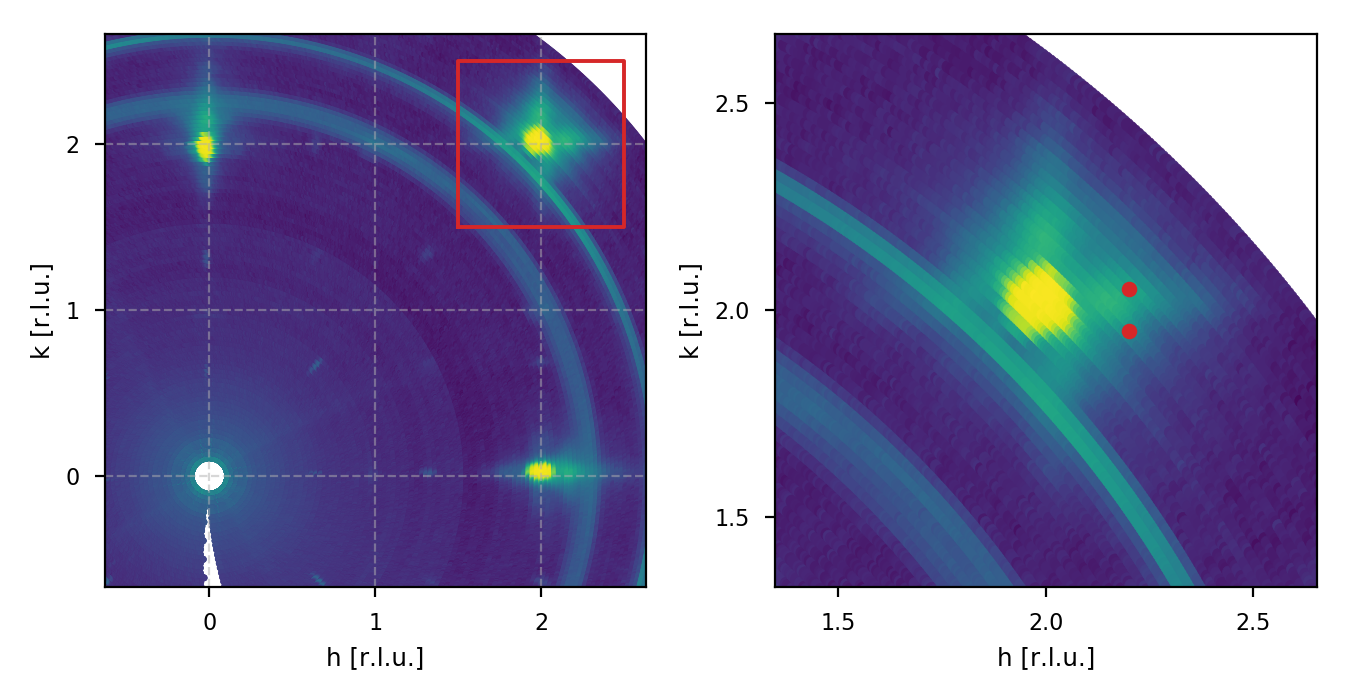
\includegraphics[width=0.9\textwidth]{fig/pdf/lscoo_ab_elastic.png}
    \caption{Reciprocal space map of single crystal La$_{1.94}$Sr$_{0.06}$CuO$_{4+\delta}$, measured in the $a$-$b$ plane with the unconventional Bmab orthorhombic coordinate system. \textbf{Left}: Full map, showing mainly the fundamental Bragg peaks. Circular arcs are powder lines from Al. \textbf{Right}: Zoomed-in view of the are marked in red, showing diffuse scattering. Thar marks are at identical locations to figure \ref{fig:lcoo_ab_elastic} as a reference for comparison.}
    \label{fig:lscoo_ab_elastic}
\end{figure}

Figure \ref{fig:lscoo_ab_elastic} shows the same type of measurement, but this time of La$_{1.94}$Sr$_{0.06}$CuO$_{4+\delta}$ on the cold TAS ThALES. While similar features are visible, the satellites seen in figure \ref{fig:lcoo_ab_elastic} are smeared out, suggesting that the tiny amount of Sr in this sample causes a significant amount of disorder which shows up as diffuse satellites.

\begin{figure}
    \centering
    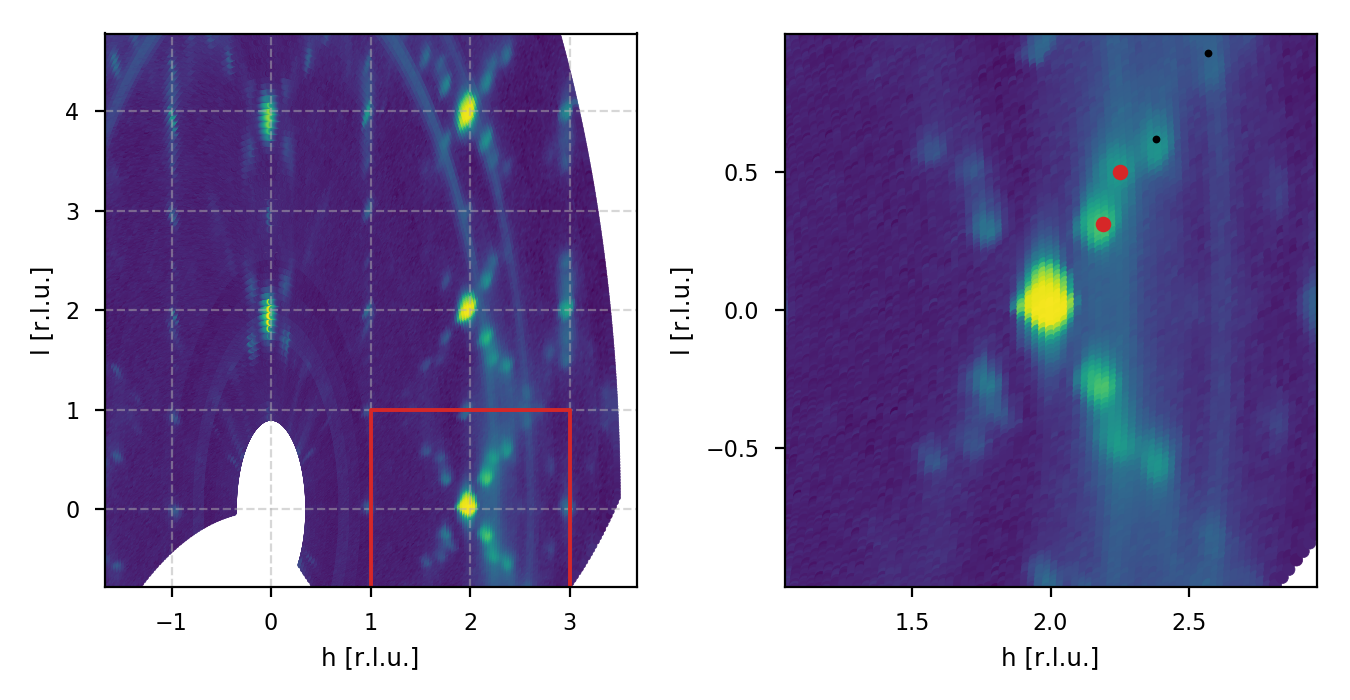
\includegraphics[width=0.9\textwidth]{fig/pdf/lscoo_ac_elastic.png}
    \caption{Reciprocal space map of single crystal La$_2$CuO$_{4+\delta}$, measured in the $a$-$c$ plane with the unconventional Bmab orthorhombic coordinate system. \textbf{Left}: Full map, showing mainly the fundamental Bragg peaks. Circular arcs are powder lines from Al. \textbf{Right}: Zoomed-in view of the are marked in red. We notice satellite peaks around (002) at $Q_2=(0.19,0,0.31)$ ($|Q_2| = \SI{0.267}{\per\angstrom}$) and $Q_3=(0.25,0,0.5)$ ($|Q_3| = \SI{0.378}{\per\angstrom}$).}
    \label{fig:lscoo_ac_elastic}
\end{figure}

Finally, in figure \ref{fig:lscoo_ac_elastic}, we show a measurement of La$_2$CuO$_{4+\delta}$ in the $a$-$c$ plane performed on ThALES. This measurement is entirely consistent with superstructures known from literature \cite{Kusmartsev2000}, and we can clearly index the peaks as $Q_2 = (0.19, 0, 0.31)$ (even showing \nth{2} and \nth{3} order reflections) and $Q_3 = (0.25,0,0.5)$. The correlation lengths associated with these peaks are $d_2 \approx \SI{24}{\angstrom}$ and $d_3 \approx \SI{17}{\angstrom}$, respectively.

While none of these measurements are new (see \cite[Chapter 10]{Ray2016}), they help to confirm that the samples we use for spectroscopic measurements in chapters \ref{ch:lowen}, \ref{ch:anomaly}, \ref{ch:arpes}. In addition, I believe it highlights an unsolved problem with regards to figuring out exactly what the nature of these structural correlations are and what (if any) relationship they have with superconductivity.

While constructing models for these superstructures is outside the scope of this thesis, they help identify some general length scales that might be relevant in a real-space model. Unfortunately, we also immediately notice that these correlations are inaccessible in our DFT MD simulations from chapter \ref{ch:md}, where the maximal simulation box is a $2 \times 2 \times 1$ cell such that the only non-zero $\bm{Q}$ we can represent is $(\frac{1}{2}\frac{1}{2}{0})$. These length scales, while rather large, are still accessible by PDF measurements as we shall see below.

\section{Real-space correlation in powders}
We now turn to experiments performed on a series of powdered samples, where we use an instrument well-suited for obtaining \emph{real-space} correlations (see section \ref{sec:specific_neutron}, chapter \ref{ch:method}) using the pair-distribution function (PDF). There are multiple purposes to this experiment. 

First, we want to simply measure oxygen-doped La$_{2-x}$Sr$_x$CuO$_{4+\delta}$ with the PDF method. From single-crystal measurements, as we saw above, it is well known that the presence of oxygen interstitials result in intricate long-range ordering phenomena. This ordering is, to my knowledge, usually not detectable in diffraction experiments on powders, but we were motivated by the fact that diffraction experiments optimized for PDF analysis are well-suited for determining correlations at \SIrange{5}{25}{\angstrom}.

Second, we wanted to see if oxygen ordering we could detect oxygen re-ordering caused by cooling rate. Single crystal measurements have shown that certain structural peaks can be removed by `quenching', that is, rapid cooling from \SIrange{300}{200}{\kelvin} in single crystal samples of La$_2$CuO$_{4+\delta}$ \cite{Poccia2012}.

\begin{figure}
    \centering
    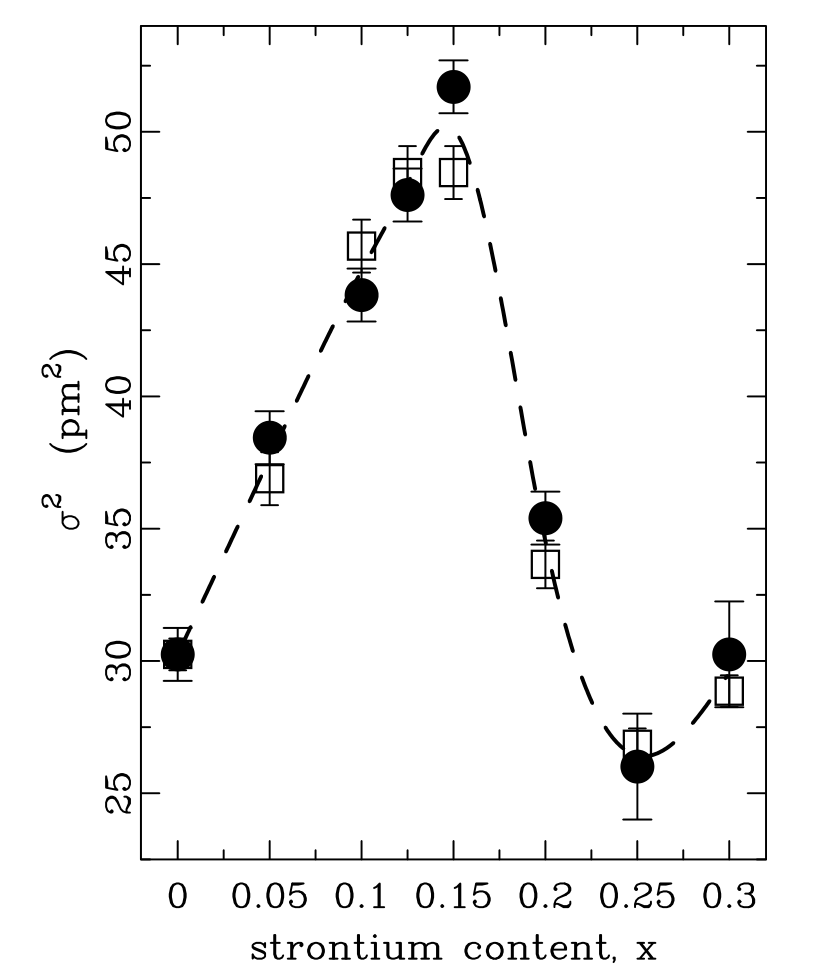
\includegraphics[width=0.4\textwidth]{fig/pdf/bozin_cuo.png}
    \caption{Relationship between strontium content $x$ in La$_{2-x}$Sr$_x$CuO$_4$ (LSCO) and the width of the Cu-O equatorial bond distribution $\sigma$. For reference, LSCO is superconducting from $x=0.05$ to $x=0.25$ and reaches the largest $T_\text{c}$ at $x=0.15$. Figure from \cite{Bozin2000}}
    \label{fig:bozin_cuo}
\end{figure}

Third, PDF measurements La$_{2-x}$Sr$_x$CuO$_4$ has shown that the \emph{distribution} of Cu-O distances is heavily influenced by doping \cite{Bozin2000}. In addition, the distribution is widest at optimal $T_\text{c}$ as shown in figure \ref{fig:bozin_cuo}. Since we are using a completely different dopant species, it is interesting to ask this same question for our samples. Finally, we want to compare high and low temperature phases to look for any peculiarities related to superconductivity or other low-temperature phases.

\subsection{Samples}
Three powdered samples were measured:

\begin{itemize}
    \item \textbf{LCO}: La$_2$CuO$_4$ (\SI{2.7844}{\gram}, insulating)
    \item \textbf{LCO+O}: La$_2$CuO$_{4.05}$ (\SI{0.7403}{\gram}, $T_\text{c} \approx \SI{40}{\kelvin}$)
    \item \textbf{LSCO3+O}: La$_{1.97}$Sr$_{0.03}$CuO$_{4.05}$ (\SI{3.3612}{\gram}, $T_\text{c} \approx \SI{40}{\kelvin}$)
\end{itemize}

\noindent Measurements were performed at the Disordered materials diffractometer D4 at Institut Laue-Langevin in Grenoble, France. Reduction and transformation of data was performed at the instrument with software specifically built for D4. All steps of the data treatment is saved, but we will mainly use the fully reduced and normalized datasets in both $Q$- and $r$-space. When comparing subtle differences between spectra (such as the same sample after different cooling procedures), we might construct a difference curve from the raw data since the background subtractions will cancel out.

\subsection{Experiment}
Table \ref{tab:measurments} contains a list of the measurements performed in the order which they were performed. The quenching was performed by submerging the \SI{300}{\kelvin} sample in liquid nitrogen and then transferring to the \SI{100}{\kelvin} cryostat. Annealing was performed by heating the cryostat to \SI{350}{\kelvin} for about an hour which is known to disorder the oxygen \cite{Poccia2012}. The reason we performed the quenching before the annealing was due to time constraints. Each acquisition was approximately 2 hours.

\begin{table}
    \centering
    \begin{tabular}{llll}
        \toprule
        index &   sample & temperature &      state \\
        \midrule
        0  &      LCO &         300 &    initial \\
        1  &    LCO+O &         300 &    initial \\
        2  &    LCO+O &         100 &   quenched \\
        3  &    LCO+O &          15 &   quenched \\
        4  &    LCO+O &         300 &   quenched \\
        5  &    LCO+O &         350 &  annealing \\
        6  &    LCO+O &         300 &   annealed \\
        7  &    LCO+O &         100 &   annealed \\
        8  &    LCO+O &          15 &   annealed \\
        9  &    LCO+O &         300 &   annealed \\
        10 &  LSCO3+O &         300 &    initial \\
        11 &  LSCO3+O &         100 &   quenched \\
        12 &  LSCO3+O &          15 &   quenched \\
        13 &  LSCO3+O &         350 &  annealing \\
        14 &  LSCO3+O &          15 &   annealed \\
        \bottomrule
    \end{tabular}
    \caption{List of measurements performed at D4 in chronological order. `Quenched' refers to the rapid cooling as described in the text, and annealing refers to keeping the sample at \SI{350}{\kelvin} for roughly 30 minutes.}
    \label{tab:measurments}
\end{table}

In summary we have a total of three samples to compare at \SI{300}{\kelvin}. For the oxygen-doped samples we can additionally look at the low temperature phase as well as the difference between `quenched' and `annealed' disorder.

\subsection{Results}
We start with the second objective of figuring out if there is any difference due to cooling procedure. Figure \ref{fig:difference} shows the difference between cooling procedures for the two oxygen-doped samples. In general there are no systematic differences apart from the slight decline of the difference curve for the LCO+O sample. This is likely due to a small amount of hydrogen in the cryostat as a consequence of the quenching procedure. The preliminary conclusion is that there is no difference between quenched and annealed measurements to a high degree of certainty. This is somewhat surprising since it is well known that certain structural peaks can be removed from quenching in single crystals \cite{Poccia2012}. We cannot conclude if our result is due to the sample being a powder or due to rotational averaging. Since we detect no difference in the spectra, we can use the annealed \SI{15}{\kelvin} data and initial \SI{300}{\kelvin} data for the remaining analysis.


\begin{figure}
    \centering
    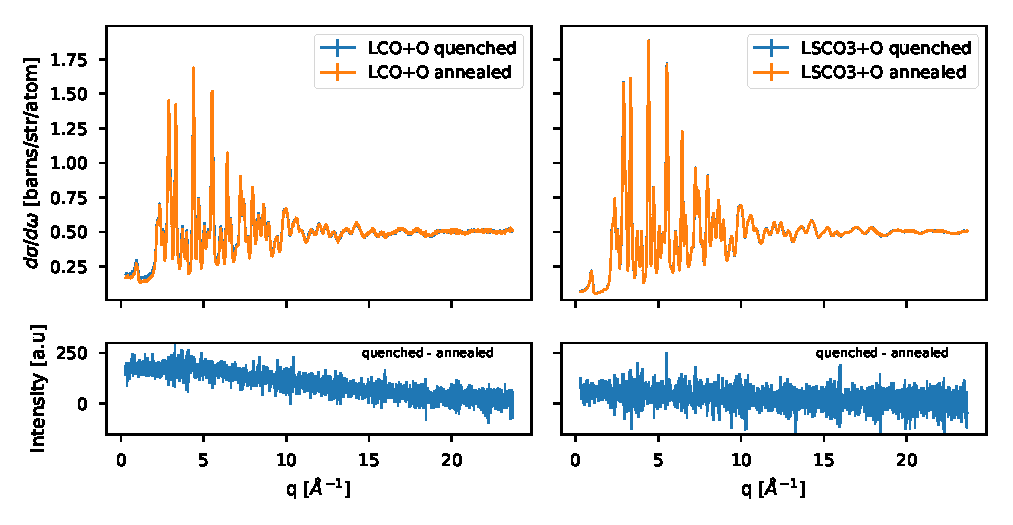
\includegraphics[width=\textwidth]{fig/pdf/quenched_annealed.pdf}
    \caption{Difference between quenched and annealed cooling procedures for LCO+O and LSCO3+O samples. The topmost plots are comparisons of the reduced and corrected $\text{d}\sigma/\text{d}\omega$ in absolute units, while the difference curves are extracted from the raw $\bm{q}$ data.}
    \label{fig:difference}
\end{figure}

In Figure \ref{fig:sample_comparision} we compare the three samples at \SI{300}{\kelvin} in both real and reciprocal space. While the differences are quite small, the difference curves (green) seem to be larger between parent/oxygenated compounds compared to the two oxygenated compounds. This is consistent with a picture where oxygen distorts the lattice in a meaningful way, while the effect of a small amount of strontium is negligible. Figure \ref{fig:temperature_comparision} shows the high- and low-temperature data for the two oxygen-doped samples. At first glance there seems to be nothing out of the ordinary, peaks are shifting slightly due to thermal expansion (this is particularly easy to spot in the real-space data).

\begin{figure}
    \centering
    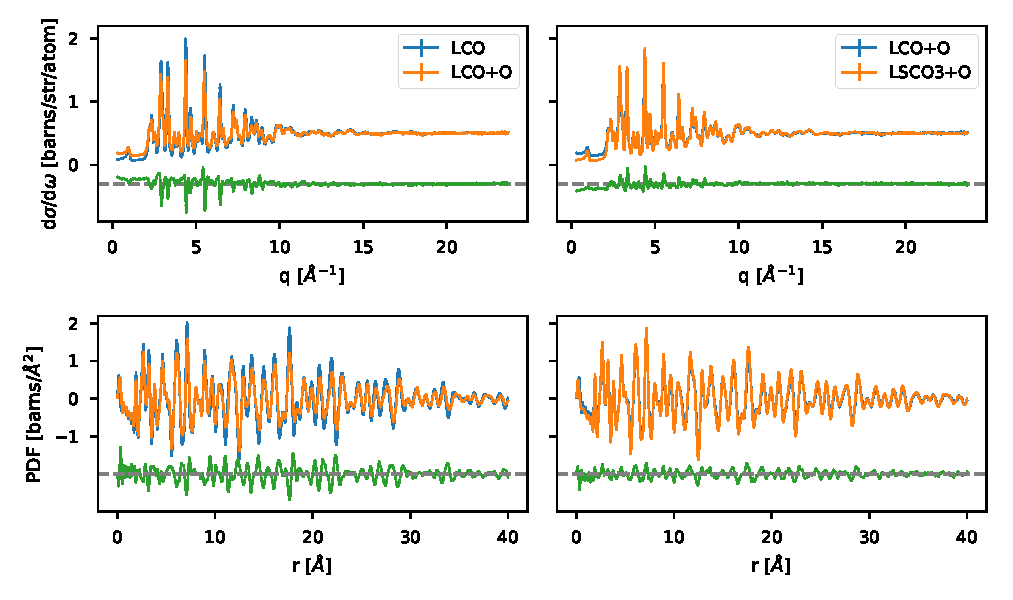
\includegraphics[width=\textwidth]{fig/pdf/sample_comparison.pdf}
    \caption{Comparison of the three different samples at \SI{300}{\kelvin} in both real and reciprocal space. On the \textbf{left} we compare LCO with LCO+O in order to see if there is an effect of oxygen. On the \textbf{right} we look at LCO+O versus LSCO3+O to have a similar comparison between two \emph{different} oxygen-doped samples.}
    \label{fig:sample_comparision}    
\end{figure}

\begin{figure}
    \centering
    \includegraphics[width=\textwidth]{fig/pdf/temperature_comparison.pdf}
    \caption{Temperature dependence of \SI{300}{\kelvin} and \SI{15}{\kelvin} for LCO+O and LSCO3+O in both real and reciprocal space.}
    \label{fig:temperature_comparision}    
\end{figure}

\subsection{Analysis}
Without performing detailed modelling, we can take a look at the first peak in the real-space data which corresponds to the Cu-O in-plane bond. This bond-length is suspected to be important for superconductivity by controlling the Coulomb interaction (the Hubbard-$U$) \cite{Ivashko2019}. Previously, as mentioned above, measurements on La$_{2-x}$Sr$_x$CuO$_{4}$ have shown that the width of the Cu-O bond-length distribution is largest at optimal doping $x=0.15$ and qualitatively tracks the superconducting dome \cite{Bozin2000}. We fit the first peak of all relevant datasets to a single Gaussian as shown in Figure \ref{fig:cu_o_fits} and report the fitting parameters in Table \ref{tab:cu_o_fits}.

\begin{figure}
    \centering
    \includegraphics[width=\textwidth]{fig/pdf/cu_o_fits.pdf}
    \caption{Cu-O distance Gaussian fits. For each of the five temperature/sample combinations (figure text), the short range PDF is shown along with a Gaussian fit of the first peak. In order to compare between the fits, the constant background has been fixed to $-1.2$}
    \label{fig:cu_o_fits}
\end{figure}

\begin{table}
    \centering
    \begin{tabular}{llll}
        \toprule
          Sample & Temperature [K] &   Cu-O mean distance &           Cu-O sigma \\
        \midrule
             LCO &             300 &  1.9010 $\pm$ 0.0003 &  0.0941 $\pm$ 0.0003 \\
           LCO+O &             300 &  1.9005 $\pm$ 0.0012 &  0.1112 $\pm$ 0.0014 \\
         LSCO3+O &             300 &  1.8995 $\pm$ 0.0003 &  0.0989 $\pm$ 0.0004 \\
           LCO+O &              15 &  1.8983 $\pm$ 0.0009 &  0.1096 $\pm$ 0.0010 \\
         LSCO3+O &              15 &  1.8944 $\pm$ 0.0003 &  0.0951 $\pm$ 0.0004 \\
        \bottomrule
    \end{tabular}
    \caption{Cu-O distances in all samples at all available temperatures as extracted from the fits in figure \ref{fig:cu_o_fits}.}
    \label{tab:cu_o_fits}
\end{table}

Comparing to La$_{2-x}$Sr$_x$CuO$_{4}$, we have roughly the same peak position at $r=\SI{1.9}{\angstrom}$. At \SI{300}{\kelvin} LCO has a smaller width compared to LCO+O and LSCO3+O. At \SI{15}{\kelvin} the widths are slightly smaller as one would expect from the reduced temperatures. Our measurements are thus consistent with the observations of \cite{Bozin2000}, but with an entirely different dopant species. Interestingly, the sample with a small amount of Sr has a slightly smaller $\sigma$.

\begin{figure}
    \centering
    \includegraphics[width=\textwidth]{fig/pdf/300k_all.pdf}
    \caption{PDF at \SI{300}{\kelvin} for the three samples studied here across the accessible range. Differences between stoichiometric and oxygen-doped samples are highlighted with grey circles. Grey vertical lines mark the correlation lengths identified in section \ref{sec:single_crystal_superstructures}.}
    \label{fig:pdf_all_300K}
\end{figure}

In figure \ref{fig:pdf_all_300K}, we take a closer look at the PDF from the three samples obtained at \SI{300}{\kelvin}. As we mentioned earlier, any differences between the plots are quite subtle, but our initial analysis that there is a `larger' difference between LCO and LCO+O when compared to the difference between LCO+O and LSCO3+O seems to be correct. Marked in figure \ref{fig:pdf_all_300K} are regions where theres is a qualitative difference between the curves. That is, we don't just see sharpening/broadening, but the shape of the peaks are noticeably different. In addition, I marked the possible correlation lengths identified in the previous section.

Unfortunately, there seems to be no real signature of a change due to interstitial that is related to the superstructures identified earlier. In addition, even though there are differences where we can clearly separate the oxygen-doped samples from La$_2$CuO$_4$, the changes that we do see are barely noticeable.

Finally, in figure \ref{fig:pdf_sim_comparision} I compare LCO and LCO+O at \SI{300}{\kelvin} with molecular dynamics simulations in the LTO phase also at \SI{300}{\kelvin} on an absolute scale. In general, we seem to have a quite good agreement between experiment and simulation, especially with regards to the short range correlations around \SI{3}{\angstrom}. Noticeably, the shortest Cu-O bond is significantly sharper in the simulation, so perhaps we are not accurately describing short range forces. At higher $r$, the simulation PDF naturally dies out due to limited system size.

\begin{figure}
    \centering
    \includegraphics[width=\textwidth]{fig/pdf/pdf_simulation_experiment_compare.pdf}
    \caption[PDF data compared with MD simulation]{PDF data compared with MD simulation}
    \label{fig:pdf_sim_comparision}
\end{figure}

\section{Summary}
In this chapter, we performed experiments with the intention of gaining a further understanding of the various superstructures present in LSCO+O. Through single-crystal measurements we independently confirmed the existence of the superstructures reported by various groups \cite{Kusmartsev2000} and additionally observed in-plane satellites only seen by us \cite{Ray2016}.

We performed high-quality PDF measurements of 3 powdered samples with and without interstitial oxygen, confirming subtle differences due to interstitials. A direct connection to the superstructures observed in single crystals could, however, not be made. If this is a consequence of superstructures not being visible in the rotationally averaged diffraction pattern or if the powders are different with regards to superstructure signatures, is hard to say. Our measurements appears consistent with the observation of \citeauthor{Bozin2000} \cite{Bozin2000} and have an increased distribution of in-plane Cu-O distances in superconducting samples, slightly more so in LCO+O compared to LSCO3+O.

Finally, the MD simulations performed in chapter \ref{ch:md} are consistent with the shape of the measured PDF, especially in the \SIrange{2}{4}{\angstrom} range. In order to properly describe the differences we see at higher correlation lengths, some real space modelling and/or reverse monte-carlo fitting of the PDF would be required to properly analyse the data. The work performed in this chapter could thus be used as a first step for constructing real-space models of non-stoichiometric oxides.


\chapter{Low Energy Lattice Dynamics}\label{ch:lowen}
In this chapter we investigate the lattice dynamics of La$_{1.94}$Sr$_{0.06}$CuO$_{4+\delta}$ as observed by neutron scattering with the intention of comparing with simulations performed in chapter \ref{ch:simulation}. Similar to the elastic reciprocal space maps done with the FlatCone analyser in the previous chapter, we now look at the same maps with finite energy transfers. These are compared to experiment by constructing neutron-weighted band structures and 2D $(Q_x,Q_y$ maps from simulation data. In addition, 

We also look at soft phonons related to the LTO-LTT transition in La$_2$CuO$_{4+\delta}$. These phonons have shown interesting behavior in LSCO, and we are interested in how this picture changes when working with oxygen-doped samples. Finally, we look at the superstructures discussed in the previous chapter and search for possibly related dynamics.

\section{Acoustic Phonons and Simulation Validation}
We start by considering measurements performed on IN8 at ILL, using the FlatCone secondary spectrometer as described in section \ref{sec:single_crystal_superstructures}. By measuring a large region of $\bm{Q}$ while changing the energy transfer $\hbar\omega$, we can build up a three-dimensional data-set of low energy phonon dispersions. The sample is a single crystal La$_{1.94}$Sr$_{0.06}$CuO$_{4+\delta}$ ($T_\text{c} = \SI{37.5}{\kelvin}$) aligned in the $a$-$b$ plane. The elastic signal was shown in the previous chapter, figure \ref{fig:lscoo_ab_elastic}. The spectroscopic measurements were performed from \SIrange{1}{16}{\milli\eV} in steps of \SI{1}{\milli\eV}.

\begin{figure}
    \includegraphics[width=\textwidth]{fig/lowen/flatcone_colorplots.png}
    \includegraphics[width=\textwidth]{fig/lowen/simulation_colorplots.png}
    \caption[Flatcone raw inelastic]{FlatCone data of La$_2$CuO$_{4+\delta}$ in the $a$-$b$ at three energies and simulation data of La$_2$CuO$_{4}$ at the same energies. \textbf{Top}: Raw data at \SIlist{6;9;12}{\milli\eV} annotated with cut directions in the leftmost figure. In addition, the middle figure highlights a small amount of spectral weight observed in a narrow range of energies near (310). \textbf{Bottom}: Simulation data at energies corresponding to the top row. Details about the simulation data is given in the text.}
    \label{fig:flatcone_raw_inelastic}
\end{figure}

Figure \ref{fig:flatcone_raw_inelastic} shows representative data at \SIlist{3;9;12}{\milli\eV} in the top row. The bottom row shows simulations results of La$_2$CuO$_4$ in the Low-Temperature Orthorhombic structural phase (see figure \ref{fig:lto_bands} for the phonon band structure along high-symmetry lines). As shown in section \ref{sec:phonon_calc}, phonon band structure calculations result in a data structure where we can obtain phonon eigenvectors at arbitrary reciprocal wave vectors $\bm{Q}$. By combining this fact with the coherent one-phonon dynamic structure factor (equation \eqref{eq:one_phonon_sqw}, we can evaluate the neutron intensity at any point in reciprocal space due to phonon scattering.

Technically, the output from a phonon calculation gives you the band structure as a list of energies, corresponding to the number of bands, at every value of $\bm{Q}$. This means that they are $\delta$-functions in 4-dimensional $(\bm{Q},\hbar\omega)$ space and we need to give them a finite with in order to produce plots as in figure \ref{fig:flatcone_raw_inelastic}. This is done by evaluating the phonons as Gaussian along the energy-axis with a width $\sigma$. Details about this implementation and the production of 2-dimensional phonon colorplots are described in appendix \ref{app:software}.

Now, as we can see in figure \ref{fig:flatcone_raw_inelastic}, there is a nice qualitative correspondence between theory and experiment. I emphasize here that the experimental and simulation data is shown without any scaling in energy. In order to quantify our experimental data, one dimensional spectra has been extracted by interpolation along the annotated directions in figure \ref{fig:flatcone_raw_inelastic} using the \texttt{nplot} software \cite{nplot}. Transverse spectra, perpendicular to $\bm{Q}$, is annotated by `T' and Longitudinal spectra, parallel to $\bm{Q}$ is annotated with an `L'. We thus have 4 sets of data -- two directions at two fundamental Bragg peaks, (220) and (400). In addition, we noticed a small amount of spectral weight at \SIrange{7}{10}{\milli\eV} at the (310) position.

\begin{figure}
    \centering
    \includegraphics[width=0.45\textwidth]{fig/lowen/dispersion_220T.pdf}
    \includegraphics[width=0.45\textwidth]{fig/lowen/dispersion_400T.pdf}
    \caption[flatcone dispersion 220T/400T]{transverse flatcone dispersions at 220 (left) and 400 (right). Fit is a simple acoustic phonon dispersion for monoatomic systems: $\omega = \sqrt{4C/M} | \sin ( \pi (q-q_0) ) | $, where $M$ is the mass $C$ is the spring constant and $q_0$ is an offset to adjust for possible misalignment of the sample. $q$ is in reciprocal lattice units.}
    \label{fig:transverse_phonons_flatcone}
\end{figure}

\begin{figure}
    \centering
    \includegraphics[width=0.45\textwidth]{fig/lowen/dispersion_220L.pdf}
    \includegraphics[width=0.45\textwidth]{fig/lowen/dispersion_400L.pdf}
    \caption[flatcone dispersion 220L/400L]{Longitudinal flatcone dispersions at 220 (left) and 400 (right). Fit is a simple acoustic phonon dispersion for monoatomic systems: $\omega = \sqrt{4C/M} | \sin ( \pi (q-q_0) ) | $, where $M$ is the mass $C$ is the spring constant and $q_0$ is an offset to adjust for possible misalignment of the sample. $q$ is in reciprocal lattice units.}
    \label{fig:longitudinal_phonons_flatcone}
\end{figure}

\begin{figure}
    \centering
    \includegraphics[width=0.8\textwidth]{fig/lowen/fits_310T.pdf}
    \caption[310T flatcone raw data]{310T flatcone raw data. The dispersion appears quite flat: $\delta_k = \{ 0.06, 0.12, 0.25, 0.35 \}$ for the 4 energies shown, with the last one (\SI{10}{\milli\eV}) being a very rough estimate from visual inspection. The direction is (400)-(220).}
    \label{fig:flatcone_phonons_310T_raw}    
\end{figure}

Figures \ref{fig:transverse_phonons_flatcone} and \ref{fig:longitudinal_phonons_flatcone} shows the peak positions as a function of energy along the transverse and longitudinal directions, respectively along with a naive fit to the shape of a monoatomic phonon dispersion \cite{Kittel2005}. Details about the peak finding feature and plots of the data is shown in appendix \ref{app:lowen_plots}. We have the expected results that longitudinal acoustic phonons are steeper since they are essentially bond stretching motions, where transverse phonons resembles a shear motion. Finally, we show the raw data for the four spectra where we see a signature of excitations around (310) in figure \ref{fig:flatcone_phonons_310T_raw}.

\begin{figure}
    \centering
    \includegraphics[width=\textwidth]{fig/lowen/flatcone_fits_simulation_lto_afm.png}
    \caption[FlatCone dispersion and neutron weighted simulation data]{Data obtained from FlatCone measurements in red (figures \ref{fig:transverse_phonons_flatcone} and \ref{fig:longitudinal_phonons_flatcone}) superimposed on the neutron-weighted simulation data of La$_2$CuO$_4$ in the orthorhombic phase. The simulation data is given a small Gaussian width in order to emphasize what a neutron experiment should look like according to simulations.}
    \label{fig:flatcone_phonons_dispersion_simulation}
\end{figure}

\begin{figure}
    \centering
    \includegraphics[width=0.5\textwidth]{fig/lowen/flatcone_fits_simulation_310T.png}
    \caption{FlatCone data of the shallow features observed in the transverse direction near (310) (figure \ref{fig:flatcone_phonons_310T_raw}), superimposed on neutron-weighted simulation data in the same direction.}
    \label{fig:flatcone_phonons_310T_sim}
\end{figure}

Once again, we can use this extracted dispersion to compare with our simulation data. In figure \ref{fig:flatcone_phonons_dispersion_simulation}, we see the data previous figures along with a neutron weighted band structure plot along the same directions. Once again, the simulations have been broadened along the energy axis in order to emphasize the neutron cross-section. This also means that there are certain bands not visible in these plots because their intensity vanishes (see figure \ref{fig:bands_sqw_color_line} for a visual explanation of this point). As indicated by the two dimensional color plot in figure \ref{fig:flatcone_raw_inelastic}, we have excellent agreement between measurement and simulation.

As the attentive reader might have noticed, we performed simulations of several different versions of La$_2$CuO$_4$ in chapter \ref{ch:simulation}. The comparison shown here is the low-temperature orthorhombic structural phase in the insulating state with static magnetism. This was chosen using through a visual inspection of the different simulations. The remaining five plots are shown in appendix \ref{app:lowen_plots}.

\begin{figure}
    \centering
    \includegraphics[width=\textwidth]{fig/lowen/simulation_colorplot_twin_comparison.png}
    \caption[Simulation comparison hkl khl]{Simulation data in the $a$-$b$ plane of La$_2$CuO$_4$ at 9 meV in the low-temperature orthorhombic phase. The first two images show the effect of exchanging the $a$ and $b$ directions when generating the plot and the last shows the superposition of the two.}
    \label{fig:lto_hk0_kh0_comparison}
\end{figure}

In addition, the bottom row of figure \ref{fig:flatcone_raw_inelastic} was generated taking twinning (see XX\todo{I should write about this early so i can refer back...}) into account. Since $a$ and $b$ directions in the low-temperature orthorhombic phase are close in length, twinning essentially makes the two directions indistinguishable. To show how this affects the dynamics, figure \ref{fig:lto_hk0_kh0_comparison} gives a visual indication of this superposition at \SI{9}{\milli\eV}. While the HK0/KH0 planes have a similar overall shape, it becomes clear that the superposition has the strongest resemblance to our data.

\begin{figure}
    \centering
    \includegraphics[width=\textwidth]{fig/lowen/twinning_plots_all.png}
    \caption[All qxqy plots at 9 meV including twinning for the LTO case]{Simulation data in the $a$-$b$ plane at \SI{9}{\milli\eV} from the six different phonon calculations performed in chapter \ref{ch:simulation}.}
    \label{fig:simulation_sqw_xy_plots_all}
\end{figure}

For the sake of completeness, figure \ref{fig:simulation_sqw_xy_plots_all} shows all six simulations from chapter \ref{ch:simulation} at \SI{9}{\milli\eV}. Once again, it seems likely that the `LTO AFM' simulation is the best representation of the sample chosen for this experiment, La$_{1.94}$Sr$_{0.06}$CuO$_{4+\delta}$.

While not groundbreaking in terms of scientific impact, I believe that these comparison confidently shows that our simulations can be trusted to some degree with regards to lattice dynamics. In addition, I hope that the tools (appendix \ref{app:software}) developed to generate these plots can be helpful for neutron scatterers in the future. To end this section, I direct the reader to a video at \url{https://youtu.be/LC-qV3CjqBM} which illustrates the dispersive features of the 2D colorplots in this section by moving through the energy axis as a function of time. While not particularly pertinent, I think it has an aesthetic most people can appreciate.

\section{Structural instabilities}
In this section, we investigate a peculiarity with regards to the low-temperature orthorhombic phase in La$_{2-x}$Sr$_x$CuO$_{4}$. In the mid 2000s, it was discovered that this material is unstable towards a low-temperature tetragonal phase at low temperatures. This shows up as the softening of a phonon at (104) and the temperature-dependence has been measured in optimally doped La$_{1.85}$Sr$_{0.15}$CuO$_4$ and insulating La$_{1.95}$Sr$_{0.05}$CuO$_4$, summarized in figure \ref{fig:soft_phonons_summary}. Back then, it was suggested that the softening abruptly stops at $T_\text{c}$ for the optimally doped sample, essentially preventing the tetragonal phase from emerging -- or at least stopping the instability in its tracks.

These ideas are consistent with the idea that lanthanum cuprates near $x=\frac{1}{8}$ have their $T_\text{c}$ suppressed due to the proximity of this tetragonal phase. This is particularly apparent in La$_{2-x}$Ba$_x$CuO$_4$ where the tetragonal phase appears and $T_\text{c}$ drops to a few Kelvin \cite{Hucker2012}.

\begin{figure}[]
    \centering
    \includegraphics[width=\textwidth]{fig/lowen/soft_phonons.png}
    \caption{Soft phonons in La$_{2-x}$Sr$_x$CuO$_4$. \textbf{Right:} Schematic of the phonons related to structural phase transitions, with HTT being high-temperature tetragonal, LTO low-temperature orthorhombic and LTT low-temperature tetragonal. Decreasing the temperature across the structural phase transition temperature $T_\text{s}$, the $X$-point phonon becomes soft and finally splits into $\Gamma$ and $Z$-point phonon branches. \textbf{Right}: Measurements of the $Z$-point phonon in La$_{1.95}$Sr$_{0.05}$CuO$_4$ and La$_{1.85}$Sr$_{0.15}$CuO$_4$, showing a softening of this mode where the phonon energy $\omega_0$ decreases with decreasing temperature. This softening is associated with a sharpening of the linewidth $\gamma$.}
    \label{fig:soft_phonons_summary}
\end{figure}

We set out to do a similar experiment on the cold Triple-Axis ThALES at ILL. The sample is a single crystal La$_2$CuO$_{4+\delta}$ aligned in the $a$-$c$ plane. Measurements were constant-$\bm{Q}$ scans, and the temperature dependence is shown in figure \ref{fig:lcoo_zpoint_phonon_fits} and the summary of the fits are shown in \ref{fig:lcoo_zpoint_phonon_energies}.

\begin{figure}
    \centering
    \includegraphics[width=\textwidth]{fig/lowen/lcoo_phonon_fits.pdf}
    \caption[lco+o Z-point phonon fits]{Measurements of the $Z$-point phonon in La$_2$CuO$_{4+\delta}$. At each temperature an energy scan from \SIrange{0.5}{5.5}{\milli\eV} is performed, clearly showing the phonon at $\approx \SI{2.5}{\milli\eV}$. The strong Bragg tail comes from the fact that we are measuring (104) and (014) simultaneously as a result of twinning. (104) is $Z$ in the orthorhombic phase, while (014) is $\Gamma$. The data is fitted to a sum of two Gaussian functions, describing the Bragg tail and phonon plus a constant background. The use of a Gasussian rather than Lorentzian for the phonon is phenological, since it described the data much better.}
    \label{fig:lcoo_zpoint_phonon_fits}
\end{figure}

\begin{figure}
    \centering
    \includegraphics[width=\textwidth]{fig/lowen/lcoo_phonon_energies.pdf}
    \caption[lco+o Z-point phonon E-T plot]{Temperature dependence of the $Z$-point phonon in La$_2$CuO$_{4+\delta}$. \textbf{Left}: Phonon energy as a function of temperature. \textbf{Right:} Phonon linewidth as a function of temperatures, where the width corresponds to the Full-Width Half-Maximum of the Gaussian.}
    \label{fig:lcoo_zpoint_phonon_energies}
\end{figure}

We immediately notice that our experiment stands out when compared to LSCO5 and LSCO15. First, the energy dependence resembles that of LSCO15, but shifted up by \SI{1}{\milli\eV} and the linewidth has the opposite dependence of what one would expect and increases with decreasing temperature. In addition the linewidth is also increased by roughly \SI{1}{\milli\eV}. I stress here that we performed these experiments with an extremely tight energy resolution (roughly $\SI{0.1}{\milli\eV}$, see figure \ref{fig:phonon_resolution}), so the broadening is definitely unique to this system.

I foresee two scenarios causing this broadening. Either it is the expected broadening that is typically observed with soft phonons or it is caused by a splitting or distribution of modes at this energy. Three factors point to the second scenario. One, we know that the interstitial oxygen in La$_2$CuO$_{4+\delta}$ is spatially inhomogeneous, so it would not be surprising to have spatially separated regions with different `spring constants' for this phonon modes. In particular, we know that this mode is related to octahedral tilts which are affected by the interstitial near the apex of the CuO$_6$ octahedra. Second, the fitting procedure revealed that a Lorentzian function gives a poor description of the data as compared to a Gaussian. While not conclusive, this points to abnormal behavior which would be in favor of the second scenario. Third, we have the opposite temperature dependance of the linewidth when compared to La$_{1.95}$Sr$_{0.05}$CuO$_4$ and La$_{1.85}$Sr$_{0.15}$CuO$_4$ which, once again, points to these measurements being anomalous when compared to the strontium doped variants.

\begin{figure}
    \centering
    \includegraphics[width=0.5\textwidth]{fig/lowen/resolution_phonons.pdf}
    \caption{Energy resolution of ThALES in the conditions used to measure soft phonons. An energy scan at an arbitrary $\bm{Q} = (0.8,0,3,8)$ close to the (104) peak we are interested in reveals an energy resolution with a $\sigma = \SI{0.04}{\milli\eV}$ Gaussian with corresponding to \SI{0.10}{\milli\eV} Full-Width Half-Maximum.}
    \label{fig:phonon_resolution}
\end{figure}

\section{Low energy modes of superstructures}
Finally, we take a look at the superstructures observed in chapter \ref{ch:local} and use the Triple-Axis Spectrometer ThALES to look for a dynamic signature of these satellites. It is well known that structural peaks, per Goldstone's theorem, should have acoustic modes emerging from their position. 

\begin{figure}
    \centering
    \includegraphics[width=\textwidth]{fig/lowen/phason_flatcone.png}
    \caption{FlatCone data of La$_2$CuO$_{4+\delta}$ in the $a$-$b$ plane in the elastic condition (top left) and at \SIlist{1;2;3;4}{\milli\eV} as indicated by the figures. In general, the energy-dependant features show no signature of superstructures, and we only see the acoustic phonon from the (200) Bragg peak.}
    \label{fig:phason_flatcone_maps}
\end{figure}

We start by looking at these dynamics with the FlatCone analyser as shown in figure \ref{fig:phason_flatcone_maps}. We, once again, clearly see the elastic scattering from the superstructures, but as we move up in energy, we only see the acoustic phonon emerging from the Bragg peak. Since the FlatCone analyser measures at a fixed energy, it can be difficult to see if the mode is very flat.

\begin{figure}
    \centering
    \includegraphics[width=0.85\textwidth]{fig/lowen/phason_colorplot.png}
    \caption[lack of phasons]{Data collected with a single-detector setup, designed to search for fundamental excitations from the satellite peaks as shown in figure \ref{fig:phason_flatcone_maps}, which also shows the direction where this data was obtained. The red and white markers indicate features visible in the individual scans, see appendix \ref{app:lowen_plots} for details. Due to the linear shape of these features, it seems likely that these are artifacts of the experiment.}
    \label{fig:lcoo_phasons_colorplot}
\end{figure}

For this reason, we switched to a single detector and made detailed measurements along the line shown in figure \ref{fig:phason_flatcone_maps}. The result is shown in figure \ref{fig:lcoo_phasons_colorplot}, revealing that we do not observe any phonon-like signature, despite very strong satellite reflections (roughly 20000 neutron counts per second). We even confirmed that we were in the best conditions possible with regards to resolution as shown in figure \ref{fig:phason_resolution}.

\begin{figure}
    \centering
    \includegraphics[width=\textwidth]{fig/lowen/resolution_phasons.pdf}
    \caption{Resolution in the experiment where we look for dynamics associated with superstructures. \textbf{Left}: Schematic of reciprocal space where we measured the energy-resolution of the instrument. I remark here that the superstructures are seen in the direction of \textbf{B}. Subfigures \textbf{A} and \textbf{B}, shows the raw data with a Gaussian fit at the two locations corresponding to the schematic. Since we are measuring close to the elastic Bragg peak, the increased intensity at \textbf{B} suggests that our resolution ellipsoid has points along the (200)-\textbf{B} direction.}
    \label{fig:phason_resolution}
\end{figure}

\section{Summary}
In this chapter, a few experiments concerning low-energy phonons were bundled together in order to help us better understand the dynamic nature of octahedral tilts in oxygen doped La$_2$CuO$_4$. We have shown that our simulations are highly reproducible in experiment, suggesting that we can expand our models to include interstitals through molecular dynamics in the next chapter. We also observed highly unusual behavior in La$_2$CuO$_{4+\delta}$ when trying to investigate soft phonons related to a structural instability. The behavior is significantly different from that of LSCO, but we still see a correlation between this phonon and $T_\text{c}$. Finally, we found no evidence of dynamics related to the well-known superstructures in La$_2$CuO$_{4+\delta}$, also highly unusual behavior.
\chapter{Lattice dynamics in LSCO+O: A study using ToF and ab-initio MD}\label{ch:in4}

\begin{framed}
    \begin{itemize}
        \item Presentation of data
        \item Comparison with simulations
        \item LTT/LTO discussion. 
        \item What does the phrase `LTT-like tilts' actually mean. Is it important?
    \end{itemize}
\end{framed}


\section{Introduction}
We are performing inelastic neutron time-of-flight experiments on a series of La$_{2-x}$Sr$_{x}$CuO$_{4+\delta}$ powdered samples in order to better understand the curious relationship between mobile (O) and static (Sr) dopants. By careful analysis of the changes in the phonon spectra, we hope to better understand the role of mobile dopants and their relationship to superconductivity.

\section{Samples}
Experiments were performed on 4 powdered samples of roughly 5 grams each: LCO (no $T_\text{c}$), LSCO (no $T_\text{c}$), LCO+O ($T_\text{c} = \SI{40}{\kelvin}$), LSCO3+O ($T_\text{c} = \SI{40}{\kelvin}$). Powders were synthesized by mixing \ce{La2O3}, \ce{CuO} and (in the case of Sr doping) \ce{SrCO3} followed by calcination in a box furnace at 950$^\circ \, \text{C}$ for 48 hours. Intercalation of oxygen was performed by electrochemical methods at University of Copenhagen. This method has previously been described elsewhere \cite{Blakeslee1998}.

\section{Experimental}
Experiments were performed at the thermal neutron time-of-flight spectrometer IN4c at Institut Laue-Langevin in Grenoble, France. In order to see excitations in the \SIrange{5}{100}{\milli\eV} range, each sample/temperature was measured at three different incident neutron wavelengths as shown in Table \ref{tab:in4_mono}. Sample was mounted in a cadmium frame as shown in Figure \ref{fig:sample_sqw}B. Each of the 4 samples was measured for 3.5-4 hours per temperature/wavelength combination. 

\begin{figure}
    \centering
    \includegraphics[width=\textwidth]{fig/gdos/sample_sqw.png}
    \caption[$S(\bm{q}, \omega)$ map and picture of sample]{\textbf{A}: $S(\bm{q}, \omega)$ map of LSCO at \SI{10}{K} with $\lambda = \SI{1.6}{\angstrom}$ incident wavelength. Data has normalized by the Bose factor. \textbf{B:} Sample mounted in cadmium frame.}
    \label{fig:sample_sqw}
\end{figure}

\begin{table}[b]
    \centering
    \begin{tabular}{lllll}\toprule
    $\lambda$ [\AA] & Monochromator  & $k$ [\AA$^{-1}$] & E [meV] & Sapphire Filter     \\ \midrule
    1.6             & PG004 & 3.93            & 31.95   & \texttt{IN}  \\
    1.1             & PG004 & 5.71            & 67.61   & \texttt{IN}  \\
    0.85            & Cu220 & 7.39            & 113.22  & \texttt{OUT} \\ \bottomrule
    \end{tabular}
    \caption[IN4: Incident energies]{Overview of incident energies used in the experiments.}
    \label{tab:in4_mono}
\end{table}

The raw time-of-flight data was reduced to $S(\bm{q},\omega)$ using the \texttt{Mantid} \cite{Arnold2014} software. Background was corrected using a Vanadium scan. Due to the isotropic nature of the powder, we only consider the magnitude of $\bm{q}$ and the resulting data can be viewed in two dimensions as shown in Figure \ref{fig:sample_sqw}A. Obtaining the density-of-states is done in Mantid with the \texttt{ComputeIncoherentDOS} algorithm, using the following expression for the 1-phonon incoherent scattering function:

 \[ S^{(1)}_{\mathrm{inc}}(Q,E) = \exp\left(-2\bar{W}(Q)\right) \frac{Q^2}{E} \langle n+\frac{1}{2}\pm\frac{1}{2} \rangle \left[ \sum_k \frac{\sigma_k^{\mathrm{scatt}}}{2m_k} g_k(E) \right]\, , \]
 
 \noindent where $\bar{W} = Q^2 \langle u^2 \rangle / 2$ with $\langle u^2 \rangle$ being the average mean-squared displacement. $n$ is the Bose factor and $E$ is the energy transfer. Finally, the term in brackets is the neutron-weighted density of states with $k$ running over the different elements in our sample. The calculated DOS is given in milibarns/steredians per formula unit per meV. The mean squared displacement was set to $\langle u^2 \rangle = \SI{0.015}{\angstrom}$, which is a good compromise between qualitatively describing our data and the actual values of $\langle u^2 \rangle$ as obtained from experiments \todo{cite hafliger} and simulations \todo{cite and create MSD figure}.
 
 In order to get meaningful results from this procedure, reduction of the raw data is usually required. Generally, one chooses a range of $Q$ and $E$ to sum over along with a re-binning of $E$. Since the measured ranges are different between incident energies, these ranges are chosen for each of the three configurations (see Table \ref{tab:in4_mono}). The parameters used for our calculations are shown in Table \ref{tab:qeranges}.
 
\begin{table}[b]
   \centering
   \begin{tabular}{llllll}
   \toprule
   $\lambda$ [\AA] & $Q_\text{min}$ [\AA$^{-1}$] & $Q_\text{max}$ [\AA$^{-1}$] & $E_\text{min}$ [meV] & $E_\text{max}$ [meV] & $\Delta E$ [meV] \\ \midrule
   1.6             & 2.0                         & 7.0                         & 4.0                  & 26.0                 & 0.2              \\
   1.1             & 3.0                         & 10.0                        & 7.0                  & 59.0                 & 0.4              \\
   0.85            & 4.0                         & 12.0                        & 15.0                 & 98.0                 & 1.0              \\ \bottomrule
   \end{tabular}
    \caption[IN4: $Q$ and $E$ windows for DOS integration]{$Q$ and $E$-ranges used in the computation of DOS. For all specta a mean squared displacement of $\langle u^2 \rangle = \SI{0.015}{\angstrom}$ was used.}
    \label{tab:qeranges}
\end{table}

\section{Results}
In order to visualize our spectra better, we start by stiching the different wavelengths together. Since the energy resolution of the instrument worsens with increasing incomming energy $E_i$ we stitch together data from the different wavelengths, such that the $\lambda = \SI{1.6}{\angstrom}$ data describes low energies up to $\approx \SI{24}{\milli\electronvolt}$, $\lambda = \SI{1.1}{\angstrom}$ data describes intermediate energies up to $\approx \SI{43}{\milli\electronvolt}$ and $\lambda = \SI{0.85}{\angstrom}$ data descibes high energy data.

Data is stitched together by chosing some cut-off energies such that no features are introduced when we combine the data. The data for $\lambda = \SI{1.1}{\angstrom}$ and $\lambda = \SI{0.85}{\angstrom}$ is then scaled such that we get a continuous spectrum across the full range. For this reason, the absolute values of the DOS is only representative for the $\lambda = \SI{1.6}{\angstrom}$ data. Figure \ref{fig:in4_stitch} shows the result of such a concatenation of data. In addition, vertical lines have been added to show qualitative features of the spectrum.

\begin{figure}
    \centering
    \includegraphics[width=\textwidth]{fig/gdos/in4_lsco3_10k.pdf}
    \caption[gDOS of LSCO3 at 10K. Visualize stitching of data.]{DOS of the LSCO3 }
    \label{fig:in4_stitch}
\end{figure}


\begin{figure}
    \centering
    \includegraphics[width=\textwidth]{fig/gdos/in4_10K.pdf}
    \caption[gDOS at \SI{10}{\kelvin}]{GDOS at \SI{10}{\kelvin}}
    \label{fig:gdos_10k}
\end{figure}

\begin{figure}
    \centering
    \includegraphics[width=\textwidth]{fig/gdos/in4_60K.pdf}
    \caption[gDOS at \SI{60}{\kelvin}]{GDOS at \SI{60}{\kelvin}}
    \label{fig:gdos_60k}
\end{figure}

\begin{figure}
    \centering
    \includegraphics[width=\textwidth]{fig/gdos/in4_300K.pdf}
    \caption[gDOS at \SI{300}{\kelvin}]{GDOS at \SI{300}{\kelvin}}
    \label{fig:gdos_300k}
\end{figure}

\begin{figure}[]
    \centering
    \includegraphics[width=\textwidth]{fig/gdos/gdos_simulation_experiment_compare.pdf}
    \caption[compare gdos simulation]{compare gdos simulation. Seems like metallic simulations are not that important for structure, but the dynamics become modified in a meaningful way!. The simulation data is smoothed by a gaussian width that depends on the energy $\sigma = 0.4 + 0.02 E$ [meV].}
    \label{fig:compare_gdos_sim}
\end{figure}
\newcommand{\LSCO}{La$_{2-x}$Sr$_{x}$CuO$_4$}
\newcommand{\LSCOOsix}{La$_{1.94}$Sr$_{0.06}$CuO$_{4.035}$}
\newcommand{\LSCOO}{La$_{2-x}$Sr$_{x}$CuO$_{4+\delta}$}
\newcommand{\LCOO}{La$_2$CuO$_{4+\delta}$}
\newcommand{\LNSCO}{La$_{1.48}$Nd$_{0.4}$Sr$_{0.12}$CuO$_4$}
\newcommand{\LSCOTwenty}{La$_{1.80}$Sr$_{0.20}$CuO$_4$}
\newcommand{\LSCOopt}{La$_{1.85}$Sr$_{0.15}$CuO$_4$}
\newcommand{\LSCOseven}{La$_{1.93}$Sr$_{0.07}$CuO$_4$}
\newcommand{\LSCOTwentyfive}{La$_{1.75}$Sr$_{0.25}$CuO$_4$}
\newcommand{\HBCOO}{HgBa$_2$CuO$_{4+\delta}$}
\newcommand{\LBCO}{La$_{2-x}$Ba$_x$CuO$_4$}
\newcommand{\LBCOtwelve}{La$_{1.875}$Ba$_{0.125}$CuO$_4$}
\newcommand{\LCO}{La$_2$CuO$_4$}
\newcommand{\Tc}{$T_\text{c}$}

\chapter{Phonon Anomalies}\label{ch:anomaly}

\begin{figure}
    \centering
    \missingfigure{left: dispersion afm/metal highlight| right: wavevectors}
    \caption{phonon anomaly simulation summary}
    \label{fig:phonon_anomaly_simulation_summary}
\end{figure}

In this chapter we focus on a specific phonon mode which has been extensively studied in the cuprates and is believed to be related to stripe order and, consequently, superconductivity. The idea is that Cu-O bond-stretching phonons interact with stripe order, causing a softening at certain wave vectors. We perform measurements of this phonon anomaly in two distinct samples of oxygen doped LSCO+O in order to establish if the anomaly is related to dopant disorder. In order to establish a connection with stripe order, we measure also measure the  phonon in high magnetic fields known to modify the spectral weight of magnetic stripes. We find that this phonon in LSCO+O has a very similar signature to that of optimally doped LSCO ($x=0.15$) and that a magnetic field of \SI{10}{\tesla} has no effect on the phonon spectral weight. Part of the material in this chapter has been submitted to Physical Review Letters. The manuscript is currently available at \href{https://arxiv.org/abs/1908.09546v1}{arXiv:1908.09546v1}.

\section{Motivation}
As discussed in the introduction (section \ref{sec:lsco}), stripe order and excitations related to stripe order appear to be ubiquitous in cuprate superconductors and in particular in the lanthanum cuprates. However, while the magnetic component of stripes have been extensively studied with neutron scattering, the charge component in this model is much more elusive. Static charge stripes only show up in superconducting samples close to the $x=\frac{1}{8}$ anomaly \cite{Tranquada1995, Tranquada1996, Christensen2014, Thampy2014, Croft2014} and direct evidence of dynamic charge stripes has only been reported for isostructural, but insulating La$_{2-x}$Sr$_x$NiO$_4$ \cite{Anissimova2014}.

If we believe that the charge rivers in the stripe model carries the superconducting current, we desperately need additional information about their behavior. For this reason, researchers have been looking for alternative methods of probing charge stripes. Additionally, since static charge order is usually associated with a suppression of superconductivity, one is naturally pushed towards understanding the fluctuations associated with static charge stripes. While the importance of `fluctuating stripes' were known early on \cite{Kivelson2003}, I believe it is fair to say that we still know were little about their behavior. Just this year (2019), evidence of dynamic charge in a large area of the cuprate phase diagram was found using resonant X-ray techniques \cite{Arpaia2019}. It has also recently been suggested that these fluctuating stripes are characterized by diffusive dynamics \cite{Mitrano2019} -- that is, the dynamics is similar to brownian motion rather than coherent oscillations (e.g. phonons).

\section{Phonon Anomalies}
Since direct, spectroscopic evidence of fluctuating charge stripes in superconducting cuprates is lacking, it may be possible to find an avenue of progress through indirect measurements. Recently, it was discovered that the dispersion of the Cu-O bond-stretching longitudinal-optical (LO) phonon in SC \LSCOopt{} (LSCO15, $T_\text{c} = 38\,\text{K}$) \cite{Reznik2007} and \LSCOTwenty{} ($T_\text{c} \approx 35\,\text{K}$) \cite{Park2014} displays a strong anomalous softening interpreted as a coupling to a novel charge collective mode \cite{Park2014}. Furthermore, merely a weak signature of the anomaly is visible in the phonon linewidth of \LSCOseven{} ($T_\text{c} \approx 15\,\text{K}$)  and \LSCOTwentyfive{} ($T_\text{c} \approx 15\,\text{K}$), suggesting that the strength of the anomaly tracks the doping-dependence of $T_c$ \cite{Park2014}. Similar phonon anomalies have been observed in Bi$_2$Sr$_2$CaCu$_2$O$_{8+\delta}$ \cite{Chaix2017}, \LBCOtwelve{} (LBCO) \cite{Reznik2006}, \LNSCO{} (LNSCO) \cite{Reznik2007} and YBa$_2$Cu$_3$O$_{6.6}$ \cite{LeTacon2014} hinting at a ubiquitous feature of cuprate superconductors.

These phonon anomalies have been extensively reviewed by \citeauthor{Reznik2012} \cite{Reznik2012} and we give just a brief overview in this chapter. In the specific case of the lanthanum cuprates, the phonon mode of interest is related to a stretching of the Cu-O bond in the CuO$_2$ plane. Figure \ref{fig:phonon_anomaly_simulation_summary} shows the calculated dispersion with the particular mode highlighted as well as the eigenvectors at $\Gamma$, $X$ and halfway between these two high-symmetry points. intuitively, we can already see why this phonon mode might be interesting to look at since the vibrational frequencies could be modified by charge modulations in the CuO$_2$ plane. In addition, phonon anomalies have been observed at exactly the charge ordering wave vector $\bm{Q}_\text{co} = \left( \frac{1}{4} \frac{1}{4} 0 \right)$ in the Bmab orthorhombic coordinate system (see XX)\todo{should probably put coordinate system in introduction, not simulation}. 

\begin{figure}
    \centering
    \inputTikZ{0.9}{fig/anomaly/phonon_1d.tex}
    \caption[1D phonon anomaly sketch]{Possible scenarios of the phonon anomaly. In the first two scenarios, only the oxygen atoms is shown and the bars represent charge stripe dynamics with the propagation as shown. In these cases the charge oscillation can be either in-phase our out-of-phase with the phonon \cite{Kaneshita2002}. In the scenario last open circles represent Cu atoms with magnetic ordering and closed circles are charge stripes running perpendicular to the chain. The static charge order then lowers the energy of the phonon \cite{Reznik2006}.}
    \label{fig:anomaly_1d}
\end{figure}

% \begin{figure}
%     \centering
%     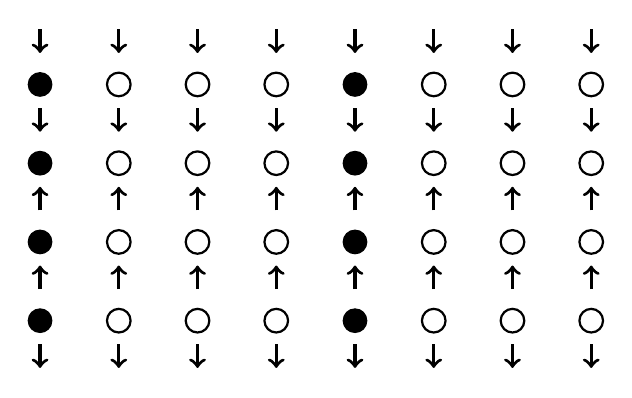
\begin{tikzpicture}
    % charge stripe
    \foreach \y in {0,1,2,3} {
        \foreach \x in {0,4} {
            \filldraw (\x+0,\y) circle [radius=0.15];
            % afm
            \draw [thick] (\x+1,\y) circle [radius=0.15];
            \draw [thick] (\x+2,\y) circle [radius=0.15];
            \draw [thick] (\x+3,\y) circle [radius=0.15];
        }
    }
    
    \foreach \x in {0,1,2,3,4,5,6,7} {
        \draw [very thick, <-] (\x,-0.6) -- (\x,-0.3);
        \draw [very thick, ->] (\x,-0.6+1) -- (\x,-0.3+1);
        \draw [very thick, ->] (\x,-0.6+2) -- (\x,-0.3+2);
        \draw [very thick, <-] (\x,-0.6+3) -- (\x,-0.3+3);
        \draw [very thick, <-] (\x,-0.6+4) -- (\x,-0.3+4);
    }
\end{tikzpicture}
%     \caption[2D phonon anomaly sketch]{Possible 2D real-space scenarios of a coupling between the Cu-O bond-stretching phonon at $q=(0.25,0.25,0)$ and stripe order. Here, the phonon wavector is perpendicular to the stripe direction (parallel to the stripe propagation vector). Small arrows represent displacement of oxygen atoms. Charge oscillations are phason modes of the stripes and the black bars represent charge domain walls. The Lower figure refers to a situation where static charge order lowers the energy of the phonon (intuitively through the change of spring constant). open circles represent hole-poor anti-ferromagnetic Cu atoms and filled circles represent hole-doped ($\frac{1}{2}$ hole per site) Cu atoms.}
%     \label{fig:anomaly_2d}
% \end{figure}

Figure \ref{fig:anomaly_1d} shows a sketch of possible scenarios involving a chain of Cu atoms (circles) separated by oxygen atoms with a certain displacement pattern (arrows). In one scenario \cite{Kaneshita2002}, the charge stripes are fluctuating and the phonon `resonates' with this fluctuation, essentially lowering its energy. In the second scenario \cite{Reznik2006}, static charge order changes the forces between certain Cu-O pairs, an effect that is also minimized at $\bm{Q}_\text{co}$ as shown in the figure. A third possibility is one where the phonon anomaly is found in the perpendicular direction to the one shown in figure \ref{fig:anomaly_1d}. In this case the phonon would resonate with the modulation `within' the charge stripe. Since the softening happens close to $\bm{Q}_\text{co}$ it seems more likely that one of the first two cases are responsible, but it has technically not been settled.

\section{Experiment}
We measured the phonon dispersion highlighted in figure \ref{fig:phonon_anomaly_simulation_summary} in two oxygenated samples: \LCOO{} and \LSCOOsix{} at the triple-axis spectrometer IN8 at ILL. Measuring this phonon dispersion turned out to be more difficult than anticipated, and several attempts were spent in order to reach optimal conditions where we could actually observe the phonon dispersion with relative success.

After our initial attempts, we realized that our signal was contaminated by so-called spurious scattering. While not immediately apparent to us, we identified this `spurion' as accidental Bragg scattering from the analyzer \cite{Shirane2002}. This means that we are in the unfortunate situations where the analyser is at angle where the sample scatters strongly from a structural Bragg peak. While the `job' of the analyser is to select a desired final energy, Bragg scattering is so strong that the signal at the detector will be contaminated by incoherent, scattering from the analyser crystals.

\begin{figure}
    \centering
    \includegraphics[width=\textwidth]{fig/anomaly/spurion.pdf}
    \caption{\textbf{Left}: Scattering triangle responsible for the A-type spurious scattering (broken lines) at $\bm{Q} = (4.7,4.7,0)$. Green points represent Bragg peaks in the ($h$,$k$)-plane. The (8,4,0) Bragg refection is responsible for the spurious scattering. \textbf{Right}: Simulated effect of the (8,4,0) reflection on a $Q$-$\hbar\omega$ map assuming a Gaussian spurious signal depending on distances in $Q$. Broken line represents a `normal' sinosoidal dispersion in this region as described in the text.}
    \label{fig:in8_spurion}
\end{figure}

Figure \ref{fig:in8_spurion} shows the geometry of this accidental Bragg scattering in reciprocal space. From this sketch we see that the spurious scattering comes from the (8,4,0) reflection. In order to quantify where we would observe this scattering in our measurements, we can make as simulation where we evaluate the strength of the spurion at the desired values of $(\bm{Q}, \omega)$. This is done by constructing the geometry as in \ref{fig:in8_spurion} (top) and then defining the spurious strength through the distance to (8,4,0). The result of such as simulation is shown in figure \ref{fig:in8_spurion} (bottom), and we clearly see that this signal intersects the expected phonon dispersion.

\begin{figure}
    \centering
    \includegraphics[width=\textwidth]{fig/anomaly/data_reduction.pdf}
    \caption{Illustration of the data reduction performed using the PSD. \textbf{Left}: Summed raw data from an energy scan at $\bm{Q}=(4.65,4.65,0)$. The dashed lines denote the regions of interest (ROI) used in the data reduction. The geometry of the instrument ensures that the desired phonon scattering will occur in the `Phonon' ROI. \textbf{Right}: Corresponding raw (diamonds) and reduced/normalized (circles) data. The raw data is obtained by only considering the `Phonon' ROI, while the reduced data is obtained by subtracting the intensity from the two `BG' ROIs. The solid line is a fit to a DHO lineshape as described in the text.}
    \label{fig:psd_data_reduction}
\end{figure}

Two measures were taken to avoid this spurious scattering. First, by using the goniometers installed on IN8 we can effectively rotate the sample around the [110] axis, which has no affect on our measurements in the [hh0] direction, but does move further away from the condition for spurious scattering since (8,4,0) will be out of the scattering plane. Second, we installed a position-sensitive detector (PSD) with the hope that the spurious scattering is spatially separated from the phonon scattering. It turns out that the spurious scattering indeed can be separated from the phonon as shown in Figure \ref{fig:psd_data_reduction}. Unfortunately, this background subtraction procedure is associated with a large increase in error bars as shown in the figure.

\begin{figure}
    \centering
    \includegraphics[width=0.49\textwidth]{fig/anomaly/fig2.pdf}
    \includegraphics[width=0.49\textwidth]{fig/anomaly/fig3.pdf}
    \caption[Phonon anomaly data and dispersion]{\textbf{Left:} Reduced data at selected wavevectors of the form $Q=(h,h,0)$ for both LSCO6+O and LCO+O at $T=5\,\text{K}$. Data at $\bm{Q}=(5,5,0)$ and $\bm{Q}=(4.85,4.85,0)$ was scaled by a factor of $\frac{1}{2}$ for clarity due to an increase of intensity from the phonon form factor. Data at different $h$ are offset for clarity. Solid lines are fits to a DHO lineshape (see text). \textbf{Right:} \textbf{(A)} Dispersion of the LO phonon obtained from the peak positions of individual spectra of both LCO+O and LSCO6+O (offset by $5\,\text{meV}$ for clarity). Error bars smaller than the markers are not shown. Dashed line is the normal sinusoidal dispersion as described in the text. All data was obtained at $T= 5 \, \text{K}$. \textbf{(B)}: Difference between sinusoidal and measured dispersion in \LCOO{} (LCO+O) \LSCOO{} (LSCO+O), \LSCOopt{} (LSCO15) and \LNSCO{} (LNSCO). Data for LSCO15 and LNSCO adapted from \cite{Reznik2007}.}
    \label{fig:anomaly_data_dispersion}
\end{figure}

Using these procedures, we were able to measure the phonon as shown in figure \ref{fig:anomaly_data_dispersion} for both \LCOO{} (LCO+O)and \LSCOOsix{} (LSCO6+O). The raw data is fit to a Damped Harmonic Oscillator (DHO) model \cite{Fak1997}, which has a Lorentzian shape:

\begin{equation}
    S(\bm{q},\omega) = I_\text{ph} \frac{1}{\pi \omega_{\bm{q}}} \frac{\gamma}{(\omega - \omega_{\bm{q}})^2 + \gamma^2} + I_\text{BG} \, ,
\end{equation}

\noindent where $I_\text{ph}$ is the phonon intensity, $\omega_{\bm{q}}$ the phonon energy at wave vector $\bm{q}$, $\gamma$ the phonon linewidth and $I_\text{BG}$ the background intensity. The extracted dispersion from the data is shown in Fig. \ref{fig:anomaly_data_dispersion} along with a normal sinusoidal dispersion, $\hbar\omega_q=\alpha \cos(2 \pi q) + \beta$, inferred from phonon calculations on LSCO using Density Functional Theory as shown in figure \ref{fig:phonon_anomaly_simulation_summary}. We fit the cosine-function to points near the zone center ($\bm{Q}=(0,0,0))$ and edge $(\bm{Q}=(\frac{1}{2},\frac{1}{2},0))$ to obtain the dashed curves of Fig. \ref{fig:anomaly_data_dispersion}A. To quantify the magnitude of the anomaly, we define the `anomaly signal' as the difference between the normal dispersion and the measured data (gray shaded area in Fig. \ref{fig:anomaly_data_dispersion}A). Fig. \ref{fig:anomaly_data_dispersion}B shows our anomaly signal for \LCOO{} and \LSCOOsix{} along with previous results from optimally doped \LSCOopt{} and insulating, stripe-ordered \LNSCO{} \cite{Reznik2007}. We emphasize the presence of similar anomaly signals on an absolute scale across all studied samples.

\section{Phonon Anomaly and Magnetic Stripe Order}
Since we have now confirmed the presence of a Cu-O bond stretching phonon anomaly in both \LCOO{} and \LSCOOsix{}, we wanted to see if this phonon dispersion could be modified by magnetic fields. The background for this idea is the fact that magnetic stripe order in \LSCO{} has a significant response to magnetic fields in a wide range of doping \cite{Chang2008,Kofu2009,Romer2013,Tranquada2004,Lake2001}. In general, the application of a magnetic field appears to `fill in' the gap of the magnetic excitation spectrum for $x \geq \frac{1}{8}$. While this, in general, is consistent with a picture where the gap is directly related to the superconducting gap, there is evidence that the filled states have a different origin \cite{Kofu2009}. Since one could write books about the spin excitation spectrum in \LSCO{}, I will keep the discussion somewhat limited and refer to the review by \citeauthor{Tranquada2013} \cite{Tranquada2013}.

\begin{figure}[]
    \centering
    \includegraphics[width=0.5\textwidth]{fig/anomaly/chi.pdf}
    \caption{Amplitude of the magnetic excitation spectrum in \LSCOOsix{} at a variety of fields and temperatures as a function of energy transfer.}
    \label{fig:lscoo_chi}
\end{figure}

Returning to the objective at hand, our idea was to both measure the spin excitation spectrum and anomalous phonons in the same experimental conditions in order to directly probe any correlation (or lack thereof) between the two phenomena. These measurements were only performed for the \LSCOOsix{} sample. Figure \ref{fig:lscoo_chi}A shows the amplitude of the magnetic fluctuations as a function of energy transfer and figure \ref{fig:lscoo_chi}B shows an example of the neutron scattering data used to extract this amplitude. The figure clearly shows that \LSCOOsix{} has gapped excitations which are filled in with the application of a magnetic field. This is in contrast to other oxygen-doped samples (e.g. \LCOO{} \cite{Jacobsen2018}) where the excitations are not gapped.

\begin{figure}
    \centering
    \includegraphics[width=0.5\textwidth]{fig/anomaly/fig4.pdf}
    \caption{Comparison of representative constant-Q ($h$,$h$,0) scans of \LSCOOsix{} in zero-field and with an applied field of $10\,\text{T}$. All measurements performed at $T=5\,\text{K}$}
    \label{fig:in8_lscoo_field}
\end{figure}

In figure \ref{fig:in8_lscoo_field} we have measured the phonon at a `normal' and anomalous wavevector at $T=\SI{5}{\kelvin}$ with and without an applied field of \SI{10}{\tesla}. From this measurement it is thus clear that a field of \SI{10}{\tesla} has no effect on the bond stretching phonon at anomalous wave vectors. 

\section{Discussion}
To begin the discussion of our results, we remark that softening and/or broadening of phonon modes is generally a signature of an incipient structural or electronic instability. Typical examples include structural phase transitions, $\bm{Q}$-dependence of the electron-phonon matrix element, Fermi surface nesting and electronic correlations \cite{Reznik2012}. In order to determine the origin of a given phonon anomaly, it is therefore important to carefully exhaust alternatives before making statements about the connection to novel phases such as dynamic charge stripes \cite{Reznik2012}.

The phonon anomaly appears in vicinity of the wave vector $\bm{Q}_\text{co}=(\frac{1}{4},\frac{1}{4},0)$, consistent with charge stripe ordering as illustrated in Fig. \ref{fig:anomaly_1d}. Measurements of LNSCO \cite{Reznik2008b}, LSCO15 \cite{Reznik2007} and LBCO \cite{Reznik2007} have shown a suppression of the anomaly as one moves away from the bond-stretching direction \cite{Reznik2008b}, supporting a one-dimensional stripe-like picture. Additionally, the phonon anomaly in LSCO15 and LBCO has almost no temperature dependence apart from a slightly sharper peak shape when heating from $10\,\text{K}$ to $300\,\text{K}$ \cite{Reznik2006,Reznik2007}. These phenomena rule out anharmonicity and structural inhomogeneity as mechanisms for the phonon anomaly in these systems.

A combination of inelastic X-ray and ARPES measurements on overdoped LSCO ($x=0.2$ and $x=0.3$) have shown that the phonon anomaly wavevector is inconsistent with Fermi surface nesting \cite{Park2013,Park2014}, contradicting the idea of a phonon softening due to a Kohn anomaly. A different, possibly $\bm{Q}$-dependent, electron-phonon coupling could still be responsible for the phonon anomaly. Such an effect would renormalize the electronic quasiparticle dispersion (the so-called `ARPES kink' \cite{Garcia2010}) at energies similar to the phonon softening. The ARPES kink has been observed in LSCO $x=0.2$ and $x=0.3$, but since only LSCO $x=0.2$ shows anomalous phonons, the two phenomena appear to not be connected \cite{Park2014}.

Thus, all previous studies are unable to explain the phonon anomaly through conventional means and any coupling to stripe order is likely dynamic. One possible scenario is a coupling of the Cu-O bond-stretching phonon with steeply dispersing charge fluctuations. \citeauthor{Kaneshita2002} performed calculations based on the Hubbard model of this scenario, predicting anomalous phonon dispersions due to both transverse (meandering) and longitudinal (compression) coherent stripe fluctuations \cite{Kaneshita2002} (see Fig. \ref{fig:anomaly_1d} for a sketch of the transverse mode). We emphasize that the observed phonon anomaly reported here (see Fig. \ref{fig:anomaly_data_dispersion}) and in LBCO/LSCO \cite{Reznik2006, Reznik2007} is remarkably similar to the calculation by \citeauthor{Kaneshita2002} (see Fig. 5 in \cite{Kaneshita2002}).

Despite differences in the magnetic excitation spectra as recorded by neutron scattering (including low and zero energy transfers), the three materials LCO+O, LSCO6+O and LSCO15 have remarkably similar in-plane Cu-O bond-stretching dispersions (Fig. \ref{fig:dispersion}). Furthermore, static charge order at zero field has been observed in a different sample of LCO+O \cite{Zhang2018} and in LNSCO \cite{Tranquada1996} but so far not in LSCO6+O nor in LSCO15. These observations together rule out a unique, direct connection between static stripes (spin and charge) and the phonon anomaly. In order to further confirm this point, we performed scans of LSCO6+O at selected wave vectors in a $H=10\,\text{T}$ magnetic field which is known to induce a considerable volume of stripe-like magnetic order in this particular sample \cite{Holm2019}. While static charge order has not been observed in LSCO6+O, measurements on LSCO ($x=0.12$) have shown that static charge and spin stripes respond identically to magnetic fields \cite{Christensen2014}.

Figure \ref{fig:in8_lscoo_field} contains data at two wave vectors with and without an applied magnetic field of $10\,\text{T}$, clearly showing the absence of any detectable field effect on the in-plane Cu-O bond-stretching phonon at $\bm{Q}=(\frac{1}{4},\frac{1}{4},0)$. These measurements were performed simultaneously with measurements of the low-energy magnetic fluctuations as shown in figure \ref{fig:lscoo_chi}, confirming a significant increase in the magnetic spectral weight towards lower energies consistent with the appearance of field-induced stripe-order \cite{Holm2019}. Thus, the appearance of static magnetic stripe order does not affect the phonon anomaly in LSCO6+O. A similar insensitivity of the phonon anomaly to an applied magnetic field has been observed in underdoped ($T_\text{c} = 66\,\text{K}$) YBa$_2$CuO$_{6.6}$ \cite{Reznik2016}.

We have shown that the phonon anomaly is a robust feature in optimally doped  as well as stripe-ordered cuprates which is independent of the structural details related to the doping process. Since it is equally well-formed in stripe-ordered and optimally doped systems, where the latter show no static magnetic order, the anomaly is surprisingly insensitive to low-energy magnetic characteristics. This is further confirmed by the absence of a magnetic field effect in LSCO6+O which introduces static magnetic stripe-order.

The phonon anomaly is strongest in the doping region around optimal $T_\text{c}$ ($0.125 \le n_\text{h} \le 0.20$) (LSCO15, LNSCO \cite{Reznik2007}, LBCO \cite{Reznik2006}, LSCO6+O, LCO+O), regardless of the presence of static charge order (LNSCO \cite{Tranquada1995}, LBCO \cite{Fujita2004}), suppression of bulk superconductivity (LNSCO \cite{Tranquada1996}) or dopant disorder (LCO+O, LSCO6+O). In addition, the phonon anomaly is unaffected by magnetic fields (LSCO6+O, YBa$_2$CuO$_{6.6}$ \cite{Reznik2016}) and temperature (LBCO, LSCO15) \cite{Reznik2007}). Thus it appears to be an intrinsic, robust signature of doped cuprates near optimal doping.

If fluctuating stripes are the fundamental degrees of freedom relevant for the cuprates, it is appealing to draw a connection to Pair-Density-Wave superconductors \cite{Fradkin2015}. In this system, the fundamental degrees of freedom are transverse charge fluctuations in an `electronic liquid crystal' phase without long range order \cite{Kivelson1998}. In this scenario, the phonon anomaly in materials without static stripe order is due to a matching of the phonon wavevector with, otherwise undetectable, short-range transverse stripe correlations. The $x=\frac{1}{8}$ anomaly then corresponds to the special case where stripes exhibit long-range order. 

In conclusion, we have measured the in-plane Cu-O bond-stretching phonon in LSCO6+O and LCO+O and provided evidence for significant anomalous behavior. Since one sample (LCO+O) exhibits charge order \cite{Zhang2018} while the other (LSCO6+O) does not \cite{Holm2019}, and since the samples also have different magnetic spectra with distinct field dependencies \cite{Jacobsen2018, Holm2019} we conclude that the phonon anomaly has no direct, trivial relationship to either magnetic or charge static order. In addition, the unique structural characteristics of oxygen-doped samples rule out a connection between the specific dopant species and the phonon anomaly. We proceed to conclude that the phonon anomaly is a signature of transverse charge stripe fluctuations, which is a common characteristic of the cuprate family and appears to be a pre-requisite to optimal superconductivity in these systems.

\section{Summary}
in this chapter we performed measurements of anomalies in a specific high energy mode possibly related to stripe order. In contrast to previous chapters, we can finally connect a feature in the phonon dynamics to superconductivity-related concepts. This is possibly due to the fact that the other measurements were less focused on specific modes and more the overall shape. Also in contrast to the previous chapters, there seems to be no difference between the anomalies discovered here and in samples with other dopants.

% \section{Origin of the phonon anomaly}
% Phonon anomalies in materials can, in general, happen for a number of reasons. The Cu-O bond-stretching phonon anomaly in LSCO does not seem to be caused by any of the conventional phenomena, and a relationship to novel charge modes has been proposed. One such charge mode is fluctuations of stripe order. The appeal of this interpretation is the near impossibility of measuring dynamic charge stripes directly. The phonon anomaly could thus provide an indirect way of investigating the elusive properties of dynamic charge stripes. Given the hypothesis that the phonon anomaly and dynamic charge stripes are related, what are then the possible mechanisms of the coupling? A couple of scenarios are given in Figure \ref{fig:anomaly_2d} and \ref{fig:anomaly_1d}.

% The charge oscilation was introduced by \citeauthor{Kaneshita2002}\cite{Kaneshita2002} in a theoretical study of stripes coupling to the phonon. The Kohn anomaly picture was introduced in context of LBCO by \citeauthor{Reznik2006}\cite{Reznik2006} as an intuitive way to explain the connection between the phonon and stripe wavevectors. The 2D picture in Figure \ref{fig:anomaly_2d} has only been mentioned (to my knowledge) by \citeauthor{Reznik2010} in his two reviews on the phonon anomaly\cite{Reznik2010, Reznik2012}. Note, it appears that the Kohn anomaly picture has been ruled out by ARPES measurements by \citeauthor{Park2014}\cite{Park2014}


% \begin{figure}
%     \centering
%     \includegraphics[width=0.7\textwidth]{fig/anomaly/fig1.png}
%     \caption[Crystal structure annotated with phonon at (0.25,0.25,0) and stripe order]{Sketch of crystal LSCO+O crystal structure containing two distinct dopants in a $4 \times 2 \times 1$ orthorhombic unit cell. The two singular Sr/O dopants correspond to a hole doping of $n_h = \frac{3}{32} \approx 0.09$. Dark blue are magnetic Cu sites while light blue represents hole-rich Cu sites. This period-4/8 segregation into charge/magnetic regions is known as stripe formation \cite{Tranquada1995}. Inset: Possible matching of stripe dynamics with the Cu-O bond stretching mode at q=$(0.25,0.25,0)$ as proposed by \citeauthor{Kaneshita2002} \cite{Kaneshita2002}.}
%     \label{fig:crystal_anomaly}
% \end{figure}

% \begin{figure}
%     \centering
%     \includegraphics[width=0.54\textwidth]{fig/anomaly/data_reduction.pdf}
%     \includegraphics[width=0.45\textwidth]{fig/anomaly/spurion.pdf}
%     \caption[IMPS data reduction and Spurion vizualisation]{\textbf{Top-left:} Raw data (summed from one constant-$Q$ scan) from the IMPS 2D detector. The phonon signal is observed in the central area and spurious signal is seen towards the edges. Broken white lines mark the areas used for data reduction. \textbf{Bottom-left:} Result of data reduction using the defined areas. We are clearly able to separate the phonon and spurious signal with this procedure. \textbf{Top-Right:} Scattering triangle responsible for the A-type spurious scattering (broken lines) at $Q=(4.7,4.7,0)$. The culprit is the (8,4,0) reflection. \textbf{Bottom-right:} Simulated effect of the (8,4,0) reflection on a $Q$-$\hbar\omega$ map assuming a Gaussian spurious signal depending on distances in $Q$. Broken line represents a `normal' (not anomalous) dispersion in this region.}
%     \label{fig:imps_data_reduction}
% \end{figure}



% \begin{figure}
%     \centering
%     \includegraphics[width=0.49\textwidth]{fig/anomaly/chi.pdf}
%     \includegraphics[width=0.49\textwidth]{fig/anomaly/field_selected.pdf}
%     \caption[LSCO6+O magnetic field effect on fluctuations and phonon]{\textbf{Left:} Imaginary part of the magnetic susceptibility in LSCO6+O as a function of energy transfer, field and temperature. As shown, a field of \SI{3}{\tesla} is sufficient to open a gap in the magnetic excitation spectrum. \textbf{Right:} Raw phonon data at anomalous ($h=4.75$) and normal $h=4.5$ wave vectors as a function of field. Contrary to the magnetic excitation spectrum, the anomalous phonon does not appear to be modified by an applied field.}
%     \label{fig:phonon_chi_field}
% \end{figure}

% \section{Things deleted from paper}

% \subsection{PDW Stuff in detail}
% As is usual with the cuprates, it is difficult to find a framework that captures all of the experimental evidence. With that in mind, we relate our findings to the concept of intertwined orders, while keeping in mind that oxygen-doped samples are macroscopically phase seperated. Intertwined orders are described with reference to pair-density-wave (PDW) superconductivity as the parent microscopic order from which $d$-wave superconductivity, magnetic order, charge order and others emerge\cite{Fradkin2015}. The PDW formalism predicts simultaneous ordering temperatures, gapless magnetic excitations\cite{Christensen2016} and an `electronic liquid crystal' phase\cite{Kivelson1998} that emerges from transverse fluctuations in the charge-density-waves (CDW) of neighbouring stripes. These fluctuations then become the fundamental degrees of freedom relevant to superconductivity. This is consistent with the fact that we see the phonon anomaly whenever the CDW is present, regardless of the nature of the transverse fluctuations. This could potentially explain the `sharper' phonon anomaly in static stripe-ordered LNSCO (Figure DISPERSION)

% %Note that I have never seen Reznik or Tranquada imply this connection, so it might be a bit too speculative?

% Returning to LCO+O, LSCO6+O and LSCO15, this would explain the discrepancy in magnetic signatures while still having similar $T_\text{c}$ and phonon anomaly, if we assume that the magnetic domains between the fluctuating stripes can be tuned separately\todo{not sure if this is the case, but in the original papers, electronic liquid phase is described without considering magnetism}. In the case of static charge order and magnetism, this is not the case\cite{Christensen2014}. Another scenario is one in as sample without separate domains of static and fluctuating stripes in which the magnetic field only modifies spectral weight at low energies while not affecting the phonon mode at $\approx 80\,\text{meV}$. A measurement of the phonon anomaly in field of static stripe ordered LSCO ($x=0.12$) would help resolve these issues. A significant disceprency in this interpretation is that fact that LSCO+O is macroscopically phase separated, so the question remains if the two phases are entirely segregated or if exactly one of them contains the physics described here\todo{Linda can you weigh in?}.

% \subsection{Chemical disorder - not sure if relevant}
% It has been suggested that the inhomogeneous charge distribution due to dopant ions can cause a renormalization of elementary excitations\cite{Park2011}. By adding optimally superconducting, oxygen-doped samples to the list of samples with strong phonon anomalies, we rule out any connection between the phonon anomaly and specific dopant disorder.

% \subsection{Discussion}
% The results of our measurements (Figure DISPERSION) clearly show the similarity of anomalous behavior between optimally doped LSCO15 and oxygen-overstoichiometric L(S)CO+O. Due to the difference in dopant species, we believe that an immediate result of these measurements is a confirmation of the relationship between fluctuating charge order in the CuO$_2$ planes and the giant phonon anomaly as proposed by \citeauthor{Reznik2012}\cite{Reznik2012}. In the following discussion, we work under the hypothesis that fluctuating charge order in LSCO15 and L(S)CO+O is expressed in the same way despite the different chemistries and bulk characteristics of the two compounds. We start by reviewing some important results from LSCO literature.

% It is well established that stripe order is ubiquitous in the cuprates, but a correlation with superconductivity remains elusive and maintaining an internal consistency between measurements is challenging. Neutron scattering, $\mu$SR, NQR and NMR experiments of $T_m$ have shown that static magnetic stripes in LSCO appear at $x=0.03$, take a maximum at $x=0.125$ (where $T_\text{c} \approx 25$ has a minimum) before disappearing abruptly\cite{Julien2003, Hirota2001}. In contrast dynamic magnetic stripes have been observed throughout the superconducting dome, with a gap opening in the spin excitation spectrum for $0.125 < x < 0.20$\cite{Kofu2009, Lee2000, Gilardi2004}. On the other hand, samples considered in this letter both exhibit static magnetic stripes\todo{REF?}, have a gap of 3 meV (LSCO+O)\todo{REF?} and no gap (LCO+O)\cite{Wells1997, Jacobsen2018}, while sharing an optimal $T_\text{c} \approx 40\,\text{K}$. With these results in mind, it is natural to question a trivial relationship between static and dynamic magnetic stripes. Recent measurements by \citeauthor{Jacobsen2018} on LCO+O show a discrepancy in the momentum-transfer of static and dynamic magnetic stripes\cite{Jacobsen2018}, directly showing that the perceived connection might be coincidental.

% If the magnetic signal from stripes occur with a modulation of $\delta_\text{m}$, the charge component appears with a modulation of $\delta_\text{c} = 2\delta_\text{m}$. In LSCO static charge stripes have been found for a narrow range of doping ($0.12 < x < 0.13$)\cite{Thampy2014, Croft2014} at the expected position with $\delta_\text{c} = 0.25$. In addition, the static magnetic and static charge stripes have an identical response to magnetic field in LSCO ($x=0.12$) below $T_\text{c}$, indicating a strong connection between the two phenomena\cite{Christensen2014}. Dynamic charge order has, to our knowledge, never been directly observed in LSCO.

% Despite the experimental inconsistencies outlined above, we believe that unifying observations of stripe order would be a significant step in our quest to understand superconductivity in the cuprates. The nature of dynamic charge order is a significant missing piece in the stripe picture. The `giant' phonon anomaly observed in LBCO, LSCO, YBCO and now L(S)CO+O represents significant progress in finding said piece. While phonon anomalies, in general, can happen for a number of reasons, the connection to stripe order comes in multiple flavours\cite{Reznik2012}. First, the phonon anomaly obeys the symmetry of charge stripes appearing at $\delta_\text{c} \approx 0.25$. The 1D nature of the phonon anomaly is verified from experiments showing a disappearance of the phonon anomaly by deviating slightly from the Cu-O bond direction\todo{REF?}. ARPES and Inelastic X-ray Scattering (IXS) experiments on LSCO ($x=0.20$)\cite{Park2014} have shown that the phonon anomaly cannot be caused by Fermi Surface nesting (Kohn anomaly). Theoretically, it has been proposed that the phonon anomaly can be explained as steeply dispersing charge fluctuations intersecting the optical phonon branch\cite{Kaneshita2002}

% Perhaps the most appealing feature of the phonon anomaly is the apparent correlation with $T_\text{c}$. In LSCO ($x=0.20$ and $x=0.15$), the anomaly amplitude is larger than for samples outside or on the edge of the superconducting dome. The samples studied in this letter follow this trend by having slightly larger $T_\text{c}$ and anomaly amplitudes compared to their LSCO15 cousin.

% With this in mind, we believe that the results contained in Figure \ref{fig:dispersion} proves the hypothesis of \citeauthor{Reznik2012} \cite{Reznik2012} that the phonon anomaly is connected to charge fluctuations in the CuO$_2$-planes. Our samples are chemically distinct to LSCO15 and each other, but exhibit identical behavior in terms of the energy scale of the phonon dispersion and the anomaly amplitude. The lack of field effect in Figure FIELD is surprising, but consistent with results on YBCO\todo{REF?}. On the other hand, the phonon anomaly has almost no temperature dependance, indicating that the fluctuations are extremely robust.

% \subsection{Old stuff 1}
% In addition, the magnitude of this gap $E_g$ has been suspected to track $T_\text{c}$ through the relation $T_c = 1.5 E_\text{g}/k_\text{B}$\cite{Kofu2009}. The samples considered in this letter contradicts this suspicion by having comparable $T_\text{c} \approx 40\,\text{K}$, while LCO+O exhibits no gap\cite{Jacobsen2018,Wells1997} while LSCO+O has a gap of $E_g \approx 3.5$ meV, similar to LSCO15\cite{Lee2000}.


% The controversy is rooted in the fact that static stripe order appears to suppress superconductivity while their fluctuations have been proposed to promote superconductivity. It thus becomes natural to ask if the static and dynamic stripe order arises from the same electronic phenomenon and if they are separate phases that can be tuned individually. 

% In either case, stripe order has manifestations of competing orders. A notorious example is the `$T_\text{c}$ anomaly' in LSCO, where a suppression of $T_c$ happens at $n_h=\frac{1}{8}$ along with measurable static magnetic and charge order\cite{Christensen2014,Croft2014,Thampy2014}, which is not present in optimally doped LSCO15. In non-superconducting, tetragonal LNSCO and LBCO, similar features have been observed\cite{Wilkins2011}. In addition, \citeauthor{Christensen2014} have shown, by performing experiments in magnetic fields, that the static charge and spin order is connected\cite{Christensen2014}.

% Fluctuating magnetic order has been extensively studied throughout the LSCO phase diagram, revealing a connection between 1) the incommensurate modulation $\delta$ of the antiferromagnetic parent phase and 2) the hole doping $n_h$. $\delta$ is equal to $n_h$ up to a saturation at $\delta = n_h = \frac{1}{8}$[yamada], once again stressing the ubiquity of this `$\frac{1}{8}$ phase' in the cuprates.

% A playground for understanding this `zoo' of orders is the LSCO+O system, which separates\cite{Mohottala2006} into distinct magnetic ($n_h=\frac{1}{8}$) and superconducting phases\cite{Udby2013}. In addition, the mobile nature of the dopants severely reduces flux pinning\cite{Mohottala2008}, indicating that annealed disorder allows the superconducting part of the sample to emerge in a cleaner way.

% From the $T_c$ anomaly in LSCO, phase separation in LSCO+O, the incommensurability $\delta$ of magnetic fluctuations and the insulating nature of LNSCO and LBCO12, we believe that the `$\frac{1}{8}$ phase' is a necessary, but not sufficient precursor for superconductivity. The question then remains: How are the magnetic and charge fluctuations related to this phase and how are they expressed in experiments?

% An appealing picture that unite these features is one of simultaneous structural and electronic phase separation in real space, with 1) the $\frac{1}{8}$ non-superconducting phase  expressed by static order and 2) the superconducting phase containing fluctuating charge and magnetic order. Due to the quenched disorder of LSCO this separation only becomes apparent around $n_h = \frac{1}{8}$, while the annealed disorder in LSCO+O results in detectable phase separation at optimal doping.

% While subtle, several experiments support this picture. \citeauthor{Kofu2009} reports a different origin of spin fluctuations in LSCO around the $\frac{1}{8}$ anomaly ($x=0.125,0.13.0.135$) above and below a spin gap at $\approx 4$ meV through detailed measurements of the intrinsic linewidth of the excitations. Recently \citeauthor{Jacobsen2018}\cite{Jacobsen2018} reported a different origin in momentum space of the static and dynamic spin stripes through high-resolution measurements of the incommensurability $\delta$ in LCO+O (The same sample studied in this letter). 

% Real-space structural phase separation in LCO+O has been probed by X-ray micro-diffraction. \citeauthor{Poccia2012} showed a spatial anti-correlation between two kinds of oxygen orderings\cite{Poccia2012} and in the single-layered cuprate HBCOO ($T_c = 95\,\text{K}$) containing oxygen interstitials, \citeauthor{Campi2015} found a nano-scale spatial anti-correlation between Oxygen-rich and CDW-rich regions\cite{Campi2015}.

% We hypothesize that novel charge fluctuations contain vital elements of the pairing mechanism in cuprates, but that SC only arises when the stripe phase is realized locally. In this picture charge fluctuations survive above $T_c$, but SC is realized only as we approach static stripe order.

% Starting from our assumption that the phonon anomaly is an expression of steeply dispersing charge fluctuations intersecting an optical phonon branch\cite{Kaneshita2002}, the above picture explains the difference between LSCO15, LNSCO and L(S)CO+O. LNSCO is close to superconductivity, but the specific local structure induced by the addition of Nd$^3+$ ions prevents the `good' charge fluctuations to separate from the $\frac{1}{8}$ phase. The stronger local energetics due to structure produces a steeper dispersion, resulting in a strongly peaked anomaly at $h=\frac{1}{4}$ (charge component of $\frac{1}{8}$ phase). LSCO15 and L(S)CO+O, on the other hand, have an optimal local structure allowing superconductivity to emerge unscathed. The slightly better superconducting properties of the oxygen-overstoichiometric samples are thus reflected in the broader and stronger anomalies. This is also consistent with the experiments performed by \citeauthor{Park2014}\cite{Park2014}, where the strength of the anomaly is found to scale with $T_c$.

% Finally, even though we are able to populate the $\frac{1}{8}$ phase with a magnetic field in LSCO+O (Udby et al, to be published) the charge fluctuations connected to SC are completely untouched by a field of 10T ($\ll H_{c2}$) and this is reflected in the absence of modifications of the anomaly (See Figure FIELD).

\chapter{Electronic Structure}\label{ch:arpes}
In this brief chapter, we take a look at the Fermi surface as measured by Angle-Resolved Photoemission Spectroscopy (ARPES) on a sample of La$_2$CuO$_{4+\delta}$. Tha majority of the experimental work was performed with assistance from Johan Chang's group at the Laboratory for Quantum Matter Research (LQMR) in Z\"urich, Switzerland. I mention in particular Masafumi Horio, who helped me prepare the samples and did all of the data analysis. I was present at the measurements, but our success would not have been possible without the expertise of the LQMR group.

While the analysis presented here is \emph{very} preliminary, I include it because it is, to my knowledge, the first ARPES experiment performed on an oxygen doped La$_2$CuO$_{4+\delta}$ sample. Since these samples are known to phase separate (see XX) electronically, we expect a superposition of a magnetic `$\frac{1}{8}$' phase and an optimally superconducting phase. It is possible that we can see some of this behavior in an ARPES experiment.

\section{Sample}
The sample is a small piece ($\approx \SI{1}{\centi\meter\cubed}$) of La$_2$CuO$_{4+\delta}$, carefully cut with the $c$-axis vertical. Before cutting the sample, we characterized it with a Laue camera and magnetization measurements as shown in figure \ref{fig:arpes_vsm}. When performing ARPES experiments, you need an atomically flat surface. Since La$_2$CuO$_4$ is a very brittle material, the only way to do this is by gluing on a small pin, knocking it off and hoping that the sample breaks in an atomically sharp way. Luckily, the 2-dimensional nature of the cuprates also translate to their structural integrity, so they are likely to cleave naturally at the CuO$_2$ interface. Before going to the ARPES experiment, the procedure was tested in the lab as shown in figure \ref{fig:arpes_cleave}.

\begin{figure}
    \centering
    \includegraphics[width=0.49\textwidth]{fig/arpes/laue2.png}
    \includegraphics[width=0.49\textwidth]{fig/arpes/vsm_lcoo.pdf}
    \caption{\textbf{Left:} Laue diffraction pattern of the La$_2$CuO$_{4+\delta}$ sample, aligned with the $c$ axis vertical. \textbf{Right:} Vibrating Sample Magnetometry (VSM) performed on a Quantum Design MPMS. Normalization performed through $\chi=4\pi \frac{\mu(1-N)}{VH_\text{app}}$, where $\mu$ is the measured signal, $V$ is the volume, $H_\text{app}$ is the applied field and $N$ is the demagnetization factor. Vertical line marks the onset superconducting transition temperature $T_\text{c} = \SI{41}{\kelvin}$}
    \label{fig:arpes_vsm}
\end{figure}

\begin{figure}
    \centering
    \includegraphics[width=0.8\textwidth]{fig/arpes/cleave.png}
    \caption{Cleaving procedure. \textbf{1:} The sample is mounted using Torr Seal Low Pressure Epoxy. \textbf{2:} A stainless steel pin ($L=6\,\text{mm}$, $d=1\,\text{mm}$) is glued to the top of the sample and subsequently \textbf{3:} knocked off with a regular screwdriver.}
    \label{fig:arpes_cleave}
\end{figure}


\section{Experiment}
ARPES experiments were carried out on the La$_2$CuO$_{4+\delta}$ sample at the Surface/Interface Spectroscopy (SIS) beamline at the Swiss Light Source. The sample was cleaved in situ at $\approx 20\,\text{K}$ under ultra high vacuum ($\leq 5 \times 10^{-11}\,\text{Torr}$) by employing the top-post technique as shown in figure \ref{fig:arpes_cleave}. Ultraviolet ARPES spectra were recorded using a SCIENTA R4000 electron analyser with horizontal slit setting. All the data were recorded at the cleaving temperature. Figure \ref{fig:arpes_fs} shows the Fermi surface map at $T=22\,\text{K}$ recorded using circularly polarized $160\,\text{eV}$ phonons.  Detailed cuts along the nodal directions with circularly polarized light is shown in Figure \ref{fig:arpes_cut1}. A comparison of different photon polarizations is shown in Figure \ref{fig:arpes_cut2}.

\begin{figure}
    \centering
    \includegraphics[width=0.8\textwidth]{fig/arpes/fermi_surface.png}
    \caption{Fermi surface of at $22\,\text{K}$ represented as raw and symmetrized data. $k_x$ and $k_y$ are in tetragonal (I4/mmm) units. The cut indicates the nodal direction as used in subsequent measurements of the band structure.}
    \label{fig:arpes_fs}
\end{figure}

\section{Discussion}
The area of the Fermi surface as shown in Figure \ref{fig:arpes_fs} corresponds to a carrier (hole) doping $n_\text{h} = 0.16$ and a hopping parameter $\frac{t^\prime}{t} \approx -0.14$, according to analysis performed by Masafumi Horio from the LMQR group.
It turns out that the measured spectra as e.g. the cut shown in Figure \ref{fig:arpes_cut1} are very similar to what was observed by the LMQR group in overdoped La$_{1.77}$Sr$_{0.23}$CuO$_4$ \cite{Horio2018}. There is thus no indication of `$\frac{1}{8}$-physics' which is generally characterized by the formation of Fermi arcs. We cannot however rule out that such arcs are not observed due to an unfavourable superposition of photoemission from the 1/8 phase and optimally doped phase in our sample.  

\begin{figure}
    \centering
    \includegraphics[width=0.8\textwidth]{fig/arpes/hs_cut1.png}
    \caption{Cut along the nodal direction (see Figure \ref{fig:arpes_fs}) with 160 eV circularly polarized photons. The subtracted background is defined by the minimum Momentum Distribution Curve (MDC) intensity at each binding energy.}
    \label{fig:arpes_cut1}
\end{figure}

Figure \ref{fig:arpes_cut2} clearly shows that we can separate the $d_{x^2-y^2}$ band from the $d_z$ band using different polarizations of light. When comparing to overdoped La$_{1.77}$Sr$_{0.23}$CuO$_4$, the band structure is very similar except that the $d_z$ band is moved down by about $\SI{0.1}{\eV}$. This could be due to an elongation of the $c$-axis, but while oxygen-doped samples are elongated when compared to the parent compound, La$_2$CuO$_{4+\delta}$ has a similar (or even smaller) $c$-axis when compared to La$_{1.77}$Sr$_{0.23}$CuO$_4$.

\begin{figure}
    \centering
    \includegraphics[width=\textwidth]{fig/arpes/hs_cut2.png}
    \caption{Cut along the nodal direction (see Figure \ref{fig:arpes_fs}) with 160 eV circular (CR), linear horizontal (LH) and linear vertical (LV) polarized photons.}
    \label{fig:arpes_cut2}
\end{figure}
%\chapter{Discussion}
\chapter{Conclusion}\label{ch:conclusion}
In this chapter, I will attempt to condense the thesis as a whole in order to discuss what was learned through the process of the various experimental and theoretical exercises. In a broad sense, the objective of this thesis is to investigate the effects of chemical disorder through different dopant species in La$_2$CuO$_4$ as introduced in chapter \ref{ch:intro} with the methods presented in chapter \ref{ch:method}. This was primarily done through DFT simulations being compared to a neutron scattering experiment. The challenge with this objective is that we know that the exact electronic structure of the cuprates, at the relevant doping levels, is an unsolved problem in condensed matter. DFT, in particular, has not been very successful in the underdoped part of the phase diagram and many-body methods are usually necessary to explain phenomena such as stripe order and fermi arcs.

\begin{figure}
    \centering
    \includegraphics[width=\textwidth]{fig/conclusion/stripe_electronic_structure.png}
    \caption{Schematic of the electronic structure as a function of hole doping $n_\text{h}$. As one moves from left to right, $n_\text{h}$ increases. On the left we have the undoped compound where there is a gap in electronic density of states due to the antiferromagnetic ground state. As doping is increased, the strong antiferromagnetic interactions are disrupted and novel phenomena such as stripe order and broken Fermi arcs emerge \cite{Keimer2015}. Finally, on the right, the hole doping is sufficient such that the material becomes a normal metal and the strong correlations are destroyed. The electronic band structures are calculated and presented in chapter \ref{ch:simulation}.}
    \label{fig:conclusion_stripe_dft}
\end{figure}

Figure \ref{fig:conclusion_stripe_dft} attempts to visualize this problem by showing how superconductivity is squeezed between localized electrons giving rise to antiferromagnetic order and a fermi liquid with itinerant electrons and a continuous Fermi surface. The solution to this problem was to simply consider the two cases available to us and perform the calculations with this drawback in mind. In some sense, we are trying to figure out how well this level of theory can explain experimental observations. Exactly for this reason, I think a crucial part of this thesis is a careful evaluation of theory with experiment -- essentially we need to know `how wrong' the theory is.

Now, we are certainly not the first to consider La$_2$CuO$_4$ within a one-electron theory. Since DFT was well-established when the high-temperature superconductors were discovered, this methodology was applied right away (see review by \citeauthor{Pickett1989} \cite{Pickett1989}). Various levels of theory have applied to La$_2$CuO$_4$, including pure Hartree-Fock \cite{Su1999}, and semi-local potentials \cite{Lane2018}. Correlated phenomena, such as stripes \cite{Anisimov2004} and broken up Fermi arcs \cite{Lazic2015, Lazic2015a} have even been calculated within DFT, albeit with ad-hoc methods such as DFT+U. 

In this thesis, I make no attempt to contribute to this discussion. Rather, I prioritize getting accurate inter-atomic \emph{forces} such that we get the best possible representation of the phonon spectrum. We thus stick to the generally accepted GGA level of theory. As we saw in chapter \ref{ch:simulation}, some experimentation lead us to the PBESol functional and a significantly increased plane-wave cutoff in order to get reasonable acoustic phonons. 

Within this framework, it was possible to get a good description of the unstable modes related to the structural phase transitions observed in La$_2$CuO$_4$. However, it turns out that the low-temperature tetragonal (LTT) phase is the `most stable' structural phase both with respect to total energy and unstable phonons. Since this LTT phase is known to be suppressing superconductivity, our calculations are consistent with a picture where superconductivity competes with this structural phase and thus prevents the structural phase transition. In this context, I remark that the isostructural, non-superconducting compound La$_2$NiO$_4$ is LTT at low temperatures \cite{Tranquada1994}.

While more experimentation with structural phases, functionals and computational parameters is always desireable, I decided to move on with the relatively successful description of phonon dynamics in La$_2$CuO$_4$ within DFT. In chapter \ref{ch:md}, we use these simulations to approach the actual objective of treating doped La$_2$CuO$_4$ as a defect structure with molecular dynamics. Our analysis of the trajectories show that oxygen interstitials tend towards a LTT-like structure, while undoped and strontium-doped compounds stay LTO-like. While our simulation box and total simulation time is somewhat limited, these results is a good indication of \emph{distinct} dynamics associated with interstitials. Importantly, these distinct dynamics are associated with a modification of the phonon density-of-states which can be observed experimentally.

\section{Oxygen Interstitial Observables}
A large part of this thesis has been dedicated to finding signatures of oxygen interstitials. As mentioned in the introduction, these materials appear to optimize the superconducting transition temperature $T_\text{c}$ and it is suspected that the mobile, interstitial nature might be important for the elevated $T_\text{c}$. As we also show in chapter \ref{ch:local}, the `annealed doping' \cite{Wells1997} associated with interstitial oxygen is mainly observed in diffraction experiments. Remarkably, our high-quality PDF measurement shows almost no signature of oxygen interstitials. The superstructures observed in single-crystal measurements are so strong that this absence must be due to either rotational averaging or because powdered samples simply don't have these superstructures.

However, the dynamics of the \emph{same} powdered samples (measured in chapter \ref{ch:in4}) does have a signature of oxygen interstitials through a broadening of the phonon DOS in the \SIrange{10}{25}{\milli\eV} range. We can qualitatively identify this broadening, through our simulations, as a signature of oxygen disorder. In the case of strontium-doping, on the other hand, we see a sharpening of features which cannot be explained through our simulations. It is possible that the electronic structure of the LSCO $x=0.03$ sample modifies the phonon spectrum in a novel way, but more experiments are required to understand the observations. The fact that we can identify the features in this manner suggests that our model captures some of the dynamics associated with interstitials. This, in extension, is evidence for LTT-like tilts in La$_2$CuO$_{4+\delta}$ in a sample that is always observed to be structurally LTO.

This intimate relationship to an incipient tetragonal phase is also observed in our measurements of soft phonons in chapter \ref{ch:lowen}. While none of these measurements are conclusive on their own, taken together they point to LTT-like behavior being important in La$_2$CuO$_{4+\delta}$ (LCO+O). To briefly recap, I have found that LCO+O features

\begin{enumerate}
    \item LTT-like tilt dynamics.
    \item Instability towards LTT which is stabilized at $T_\text{c}$.
    \item Phase separation into distinct $n_\text{h}=\frac{1}{8}$ and optimally superconducting phases \cite{Mohottala2006,Udby2013}.
\end{enumerate}

\noindent Allowing myself to speculate wildly, this is consistent with a scenario where La$_2$CuO$_{4+\delta}$ is able to optimize the relationship between a stripe phase and a superconducting phase by leveraging LTT-like tilts. In this way, the annealed oxygen order, optimally superconducting phase can be `close' to the static stripe phase without actually being pinned by LTT symmetry. This is consistent with a situation where `stripe degrees of freedom' are necessary for superconductivity, but where we need to be sufficiently far away from static order. Essentially, one could think of a situation where the mobile dopants in La$_2$CuO$_{4+\delta}$ self-organize in a way that optimizes the conditions for these competing orders. A similar idea has been put forward by \citeauthor{Poccia2017} \cite{Poccia2017}, where it is suggested that grain boundaries help optimize this mechanism.

\section{Phonons and Stripes}
The relationship to stripe order in LCO+O was also investigated through measurements of the phonon anomaly in chapter \ref{ch:anomaly}. Contrary to what we saw in the preceding chapters, the phonon anomaly appears to be unrelated to the type of dopant or stripe order. In fact, when reviewing the samples where the phonon anomaly has been observed it appears to be a signature of doping $0.12 < n_\text{h} < 0.20$.

We interpret this as fluctuations of charge stripes, i.e. the stripe degrees of freedom mentioned above. Following the logic from before, this then suggests that charge fluctuations are a necessary but not sufficient condition for optimal superconductivity. In addition, the anomaly persists to high temperatures, so the phenomenon must be intrinsic to the doped samples in a large temperature range.

Very recently, resonant X-ray methods were used to determine `charge density fluctuations' (CDF) in samples of YBa$_2$Cu$_3$O$_{7-\delta}$ and Nd$_{1+x}$Ba$_{2-x}$Cu$_3$O$_{7-\delta}$ over a large doping range. Similar to what has been observed in the phonon anomaly, the CDF's are constrained in the phase diagram, but persists well above the pseudogap temperature $T^*$. Figure \ref{fig:cdw_summary} shows a summary of their results and a schematic of where one finds the phonon anomaly. The similarity of these phenomena strongly supports the suggested \cite{Reznik2012} connection between the phonon anomaly and dynamic stripes.

Finally, we discovered that the electronic structure as observed by ARPES in La$_2$CuO$_{4+\delta}$ is remarkably similar to that of overdoped La$_{1.77}$Sr$_{0.23}$CuO$_4$. Since La$_2$CuO$_{4+\delta}$ is known to phase separate into stripe ordered and superconducting phases, this is interpreted as a superposition of the two phenomena in the ARPES spectrum in chapter \ref{ch:arpes}

\begin{figure}
    \centering
    \includegraphics[width=\textwidth]{fig/conclusion/cdw_summary.png}
    \caption{\textbf{Left:} YBa$_2$Cu$_3$O$_{7-\delta}$ and Nd$_{1+x}$Ba$_{2-x}$Cu$_3$O$_{7-\delta}$ phase diagram showing charge fluctuations in a wide doping/temperature range \cite{Arpaia2019}. \textbf{Right:} Schematic of where the phonon anomaly appears in a generalized cuprate phase diagram (see dicussion in chapter \ref{ch:anomaly}).}
    \label{fig:cdw_summary}
\end{figure}

% \section{Outlook}
% In more concrete terms, I would propose the following research projects:

% \begin{enumerate}
%     \item An extended study of forces in Cuprates using DFT based on our results. Are there other functionals or higher-level theories that might be important in the evaluation of forces. Could include other cuprates to test for generality.
%     \item Classical molecular dynamics of LCO+O. Since DFT limits the size of our simulations box, it could be interesting to construct a large supercell and investigate if the observed superstructures emerge. Forces could be evaluated from the DFT calculations performed here.
%     \item A study of the observed superstructures in La$_2$CuO$_{4+\delta}$ and La$_2$NiO$_{4+\delta}$. Perhaps reverse monte-carlo methods or 2D PDF could be used to solve these structures.
% \end{enumerate}





\appendix

\lstset{basicstyle=\ttfamily\footnotesize, breaklines=true, frame=single}

\chapter{Phonopy tutorial}
In practice, the procedures outlined in this chapter\todo{refer to chapter/section} are sufficiently general such that the calculation of phonon band structures can be performed by a computer program with minimal human interference. In the following example, I will show how phonons are calculated in the HTT phase of LCO using Phonopy and VASP.

\section{Starting Structure}
To begin, you need to know the space group and fractional coordinates of the structure. These are usually determined experimentally through diffraction experiments and can be found in various databases (such as the ICSD [REF?]). For VASP to understand the input structure, it is necessary to convert the downloaded file (usually .cif) into POSCAR format using e.g. VESTA. Since both Phonopy and VASP automatically determines symmetry, the starting structure does not need to be primitive. In this example we use LCO in the orthorhombic coordinate system wth the HTT symmetry (La$_8$Cu$_4$O$_{16}$)

\section{Geometry optimization}
Phonon calculations assumes equilibrium, so it is required to run a geometry optimization in VASP so forces on atoms are minimized prior to displacement generation. There are a few strategies for a successful optimization, see Section XX. Phonon calculations, in general, require accurate forces, so it is recommended to increase the precision significantly. It is typical to set \texttt{EDIFF=1e-8}, \texttt{LREAL=F}, \texttt{PREC=A}, \texttt{ENCUT=800} and to use a mesh density of $\geq 5000$ $k$-points per reciprocal atom. While there is some value in performing the geometry optimization in the supercell used for phonon calculations, this is usually unnecessary and costly in terms of computational time.

\section{Generate displacements}
From the optimized structure, one generates a set of displacements sufficient to populate the dynamical matrix. This is automatically determined by Phonopy and the only user defined parameter is the supercell expansion. Here, we are usually limited by the poor scaling of DFT calculations with respect to system size (effectively $O(n^2 \ln n)$ \footnote{https://scicomp.stackexchange.com/questions/5515/how-does-density-functional-theory-scale-with-system-size}[citation needed]). A typical reasonable size is a few hundred atoms and/or a cube with side length \SIrange{10}{15}{\angstrom}. For this example, we expand the orthorhombic unit cell to a $2 \times 2 \times 1$ super cell with a size of $\SI{10.6}{\angstrom} \times \SI{10.6}{\angstrom} \times \SI{13}{\angstrom}$ and 112 atoms. In order to generate the displacements, one uses the Phonopy command
\begin{lstlisting}
phonopy -c POSCAR -d --dim="2 2 1" --magmom 1 -1 1 -1 0 0 0 0 0 0 0 0 0 0 0 0 0 0 0 0 0 0 0 0 0 0 0 0
\end{lstlisting}

\noindent where \texttt{POSCAR} is the input file. The (optional) \texttt{magmom} tag takes magnetism into account and the 28 numbers correspond to the collinear magnetic moments of each atom. In this example they correspond to the AFM structure of LCO. Including magnetism increases the number of displacements since time-reversal symmetry is broken on neighbouring Cu atoms. The phonopy command generates a number of new \texttt{POSCAR-XXX} files to be used in DFT calculations. In addition, if the magmom tag was specified, a \texttt{MAGMOM} file is generated, providing the magnetic moments of each atom in the supercell.

\section{Run DFT calculations}
One DFT single-point calculation is performed on each of the displaced supercells \texttt{POSCAR-XXX}. Since we are trying to determine forces due to small displacements, high precision is essential. In addition, we can significantly reduce the generated data from the simulation by setting \texttt{LWAVE=F}, \texttt{LCHARG=F}, \texttt{LORBIT=10} and \texttt{LDAUPRINT=0}. The mesh density should be scaled according to the supercell size. In our example we use a $8 \times 8 \times 4$ $k$-point mesh for the original cell and $4 \times 4 \times 4$ for the supercell.

\section{Generate force constants}
Force constants are generated by reading \texttt{vasprun.xml} files from the simulations. The Phonopy command is
\begin{lstlisting}
phonopy -f 01/vasprun.xml 02/vasprun.xml 03/vasprun.xml ...
\end{lstlisting}

\noindent where the \texttt{vasprun.xml} files are listed in the same order as the \texttt{POSCAR-XXX} files that generated them. This procedure generates the force constants, and we have all the information necessary to obtain phonon eigenvalues and eigenvectors.

\section{Saving and Distributing}
At this point, we can generate phonon band structures, density of states, thermodynamic properties and visualize phonon modes. For details, I will refer to the Phonopy website [REF\footnote{https://atztogo.github.io/phonopy/}] and the excellent phonon visualization website [REF\footnote{http://henriquemiranda.github.io/phononwebsite/index.html}]. The data needed to construct the dynamical matrix is fully contained in the \texttt{FORCE\_SETS} and \texttt{phonopy\_disp.yaml} files. While these files are sufficient to distribute phonon data, it is useful to include the computational parameters geometry optimization and phonon calculations.

\chapter{PhononNeutron - Comparing Simulation and Experiment}
During the thesis, a selection of python classes were developed with the intention of generalizing some of the tasks required to get the correct neutron weights out of simulations. While software such as MDANSE does a good job with respect to molecular dynamics, I wanted something focussed on analysing phonons specifically from different levels of theory (MD and `Frozen Phonons').

The code be found at \url{https://github.com/tejsner/phonon_neutron} along with installation instruction. The intention of this appendix is to explain some of the functionality and to serve as a tutorial for anyone interested in performing the same kind of analysis.

\chapter{Structural Transformation Matrices}

Conventional Cells (Bmab and P4$_2$/ncm are identical so this transformation is the identity)

\[
\text{I4/mmm} \quad 
\begin{pmatrix}
1 & \bar{1} & 0 \\
1 & 1 & 0 \\
0 & 0 & 1
\end{pmatrix}
\quad \text{Bmab}
\]

\noindent Primitive Cells

\[
\text{I4/mmm} \quad 
\begin{pmatrix}
1 & 1 & 0 \\
1 & \bar{1} & 0 \\
1 & 0 & \bar{1}
\end{pmatrix}
\quad \text{Bmab} \quad
\begin{pmatrix}
1 & 0 & 1 \\
0 & 1 & 0 \\
\bar{1} & 0 & 1
\end{pmatrix} 
\quad \text{P4}_2\text{/ncm}
\]

\chapter{Additional Data}
This appendix contains plots and analysis that would be distracting in the main text, but are important to reference in any thorough investigation.

\chapter{VASP Inputs}

\begin{figure}
    \centering
    \begin{lstlisting}[basicstyle=\footnotesize\ttfamily, frame=single]
    ENCUT = 520 # 1.3x suggested value from O POTCAR, 800 for phonons
    EDIFF = 1E-5 # 1E-8 for phonons
    ALGO = NORMAL
    PREC = Accurate
    ADDGRID = .FALSE.
    LREAL = Auto # Switch to .FALSE. for phonons
    
    GGA = PS # PBESol functional, PE switches to default PBE
    
    ISPIN = 2
    MAGMOM = 1 -1 1 -1 24*0 # AFM structure
    
    IBRION = -1 # Single point calculation
    NSW = 0     # Number of ionic steps
    
    ISMEAR = 0
    SIGMA = 0.1
    
    LDAU= .TRUE. # Enable LDA+U with U=8eV and J=0.8eV
    LDAUTYPE = 4 # No exchange splitting
    LDAUL = 2 -1 -1 # only on Cu d states
    LDAUU = 8 0 0 
    LDAUJ = 0.8 0 0
    \end{lstlisting}
    \caption[VASP: Typical INCAR]{Typical INCAR for VASP simulations.}
    \label{fig:incar}
\end{figure}


\printbibliography

\end{document}
